\section{Introduction and Motivation: Why Language Models Are Reshaping Temporal Modeling}\label{introduction-and-motivation-why-language-models-are-reshaping-temporal-modeling}

The impact was immediate. Within twelve months, two adjacent paradigms emerged. The first, \textbf{language-centric} LLM4TS, kept the LLM frozen or partially fine-tuned via low-rank adapters and concentrated on the numeric-to-token interface (PromptCast {[}10{]}, TEST {[}11{]}, CALF {[}12{]}, TimeCMA {[}13{]}, AutoTimes {[}14{]}). The second, \textbf{numeric-centric} time series foundation models (TSFMs), abandoned the text backbone and instead trained Transformer-style models from scratch on enormous numerical corpora, treating ``time series'' as its own modality. \textbf{Chronos} (Ansari et al., 2024) {[}15{]} from Amazon tokenised continuous values into a 4096-bin vocabulary and fine-tuned T5; \textbf{TimesFM} (Das et al., 2023) {[}16{]} from Google trained a 200 M-parameter decoder-only model on 100 billion time points; \textbf{Lag-Llama} (Rasul et al., 2023) {[}17{]} adopted a LLaMA-style decoder with lag-feature inputs; \textbf{Moirai} (Woo et al., ICML 2024) {[}18{]} from Salesforce introduced any-variate attention and probabilistic outputs; \textbf{MOMENT} (Goswami et al., ICML 2024) {[}19{]} from CMU released encoder-only models for general analysis; \textbf{Time-MoE} (Shi et al., 2024) {[}20{]} scaled to 2.4 B parameters via sparse mixture-of-experts; \textbf{Timer} {[}21{]} and \textbf{Sundial} {[}22{]} explored generative pretraining and flow-matching objectives.

\begin{figure}
\centering
\pandocbounded{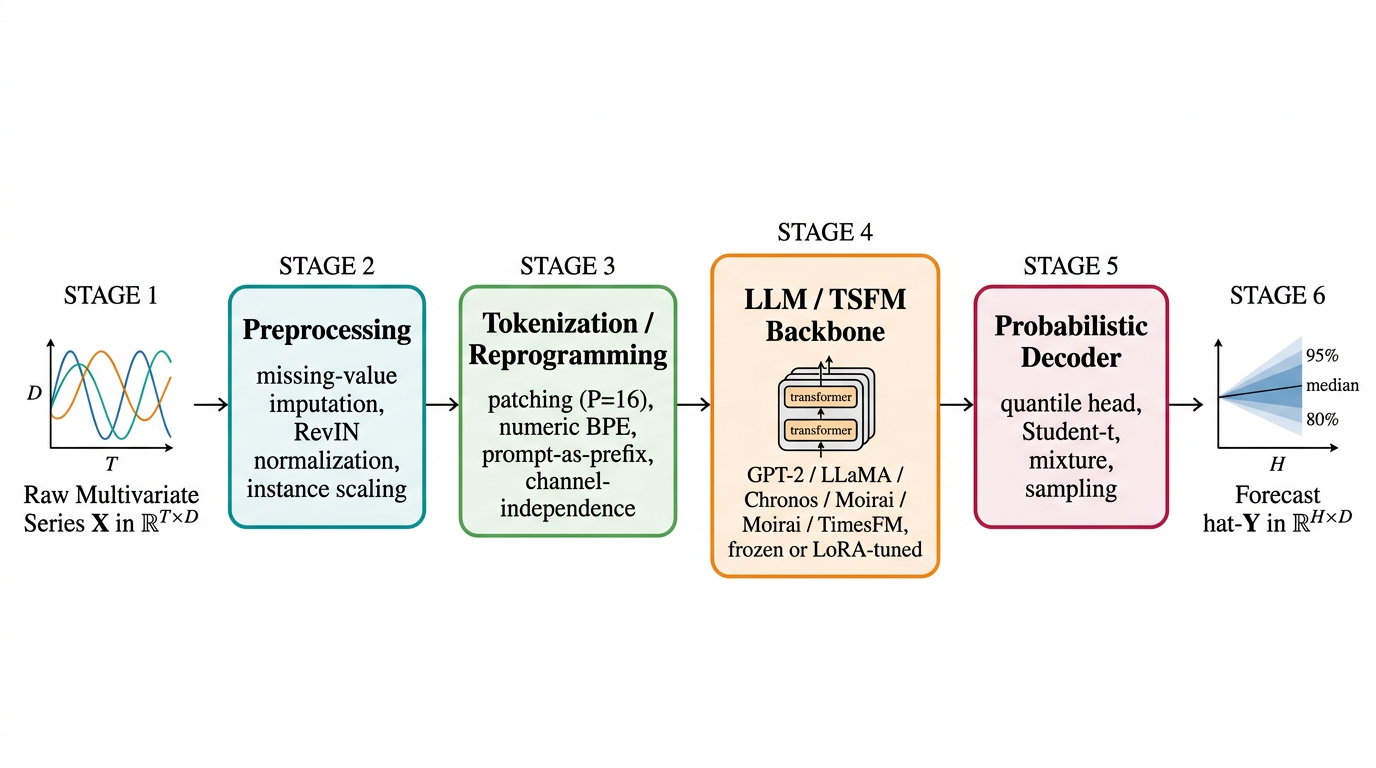
\includegraphics[keepaspectratio,alt={Pipeline overview: from raw multivariate series, through preprocessing, tokenization or reprogramming, into an LLM/TSFM backbone, to a probabilistic horizon-H forecast.}]{./figures/Large-Language-Models-for-Time-Series__fig1_pipeline.png}}
\caption{Pipeline overview: from raw multivariate series, through preprocessing, tokenization or reprogramming, into an LLM/TSFM backbone, to a probabilistic horizon-H forecast.}
\end{figure}

By late 2024 the field had accumulated enough breadth and depth that several survey efforts became necessary. Zhang et al.'s IJCAI 2024 paper ``Large Language Models for Time Series: A Survey'' {[}23{]} proposed a five-axis taxonomy. Liang et al.~(KDD 2024) ``Foundation Models for Time Series Analysis: A Tutorial and Survey'' {[}24{]} focused on TSFMs with 152 citations within a year. Jiang et al.~``Empowering Time Series Analysis with Large Language Models'' {[}25{]} catalogued reprogramming techniques, while Su et al.~systematically reviewed forecasting and anomaly detection LLMs {[}26{]} and Miller et al.~synthesised the broader deep-learning-plus-foundation-model landscape {[}27{]}. Domain-specific surveys appeared in parallel: Ansari et al.~on transformers and LLMs for ECG {[}28{]}, Liu et al.~(Expert Systems with Applications, 2026) on medical time series LLMs {[}29{]}, Ferrara on wearable-sensor LLMs {[}30{]}, Lu on financial TSFMs {[}31{]}, and Xi et al.~on disruptive impacts in management forecasting {[}32{]}. The rapid release of unified benchmarks --- \textbf{TFB} (Qiu et al., VLDB 2024) {[}33{]}, \textbf{GIFT-Eval} (Aksu et al., 2024) {[}34{]}, and \textbf{TSFM-Bench} (Li et al., KDD 2025) {[}35{]} --- has begun to discipline a previously fragmented evaluation culture.

Yet the field is not in equilibrium. A pivotal NeurIPS 2024 ablation study by Tan, Merrill, Gupta and colleagues, ``Are Language Models Actually Useful for Time Series Forecasting?'' {[}36{]}, showed that for several headline LLM-based forecasters, replacing the LLM body with random initialisation, attention shuffling, or even removing the LLM entirely failed to degrade accuracy and sometimes improved it. Edwards et al.'s scaling-laws paper {[}37{]} confirmed power-law improvements on numeric pretraining loss but found a much shallower transfer to downstream task accuracy than is observed in NLP. Xu et al.~{[}38{]} reported that supervised baselines such as PatchTST often equal or beat specialised foundation models on canonical long-term benchmarks. These results do not invalidate the LLM4TS direction, but they do reframe the central scientific question of the field: \emph{under which precise conditions does language pretraining or large-scale numerical pretraining provide measurable benefit, and what mechanisms --- patching, tokenisation, channel handling, or distributional output --- are doing the actual work?}

This survey synthesises the rapidly accumulating literature, arranged as follows. Section 2 establishes the conceptual vocabulary, formal problem statements, and classical baselines that any LLM4TS method must surpass. Section 3 introduces a five-family taxonomy spanning prompt-based, reprogramming, frozen-backbone, numeric-token, and patch-continuous approaches. Section 4 traces the compressed history from Vaswani's Transformer in 2017 through Moirai 2.0 in 2025. Section 5 dissects the algorithmic mechanisms --- patching, RevIN, numeric tokenisation vocabularies, prompt-as-prefix, mixture-of-experts routing, and probabilistic heads. Section 6 catalogues the datasets, pretraining corpora, and benchmark suites that form the field's empirical infrastructure. Section 7 examines evaluation metrics, calibration, and statistical pitfalls, with explicit attention to MASE, CRPS, weighted quantile loss, and the leakage and look-ahead problems documented by Hewamalage et al.~{[}39{]}. Section 8 surveys six application domains (energy, finance, healthcare, epidemiology, climate, mobility) with concrete deployments. Section 9 discusses limitations and failure modes including the Tan et al.~ablation findings and the ``hidden simple baseline'' pathology. Section 10 articulates open problems and falsifiable predictions for the 2026--2028 horizon. Section 11 concludes.

Three threads run throughout. First, \emph{retrievability}: every named method, dataset, score, and limitation is anchored to a paper, year, and venue so that downstream readers and quiz-style evaluators can find concrete answers. Second, \emph{honesty about negative results}: we discuss when LLMs help, when they do not, and which seemingly impressive numbers reduce to the contribution of patching, instance normalisation, or simple linear baselines (Zeng et al.~2023 {[}6{]}; Tan et al.~2024 {[}36{]}). Third, \emph{cross-disciplinary breadth}: while the most active LLM4TS research is in machine learning conferences, the highest-stakes deployments are in healthcare (Makarov et al., npj Digital Medicine 2025 {[}40{]}), public health (Du et al., Nature Computational Science 2025 {[}41{]}), and energy. The survey deliberately weaves these domains together rather than relegating them to a closing application section.

The fundamental question of the field is whether time series and natural language are sufficiently similar at a representational level for the same Transformer backbone to serve both, or whether the apparent successes of LLM4TS are artefacts of patching, normalisation, and the rich-data regime. This survey provides the evidence and taxonomy needed for readers --- researchers, practitioners, reviewers, and policymakers --- to form a defensible position on that question and to design the next generation of experiments that will resolve it.

\section{Conceptual Foundations: From ARIMA to Token-Based Temporal Reasoning}\label{conceptual-foundations-from-arima-to-token-based-temporal-reasoning}

Building on the motivation in Section 1, this section turns to the formal vocabulary the survey will use. This section reviews problem statements, classical baselines, benchmarks, tokenization choices, notation, and the case for language priors, organized as seven subsections that prepare the taxonomy in Section 3. Representative classical baselines anchored throughout include: ARIMA (1970s, parametric Box--Jenkins differencing model), ETS / Holt--Winters (1980s, exponential smoothing of level/trend/seasonality), Theta (Assimakopoulos \& Nikolopoulos 2000, M3 competition winner), Prophet (Taylor \& Letham 2018, Bayesian additive decomposition with holidays), DeepAR (Salinas et al.~2017, global LSTM probabilistic forecaster), N-BEATS (Oreshkin et al.~2020, residual MLP stack), and N-HiTS (Challu et al.~2023, hierarchical interpolation extension).

\subsection{Formal Problem Statements}\label{formal-problem-statements}

A \emph{time series} is a sequence \(x_{1:T} = (x_1, x_2, \ldots, x_T)\) where each \(x_t \in \mathbb{R}^D\) is a \(D\)-dimensional vector observed at time index \(t\), drawn from an underlying (often non-stationary) data-generating process. When \(D=1\) the series is \emph{univariate}, otherwise \emph{multivariate}. The standard tasks an LLM4TS or TSFM system must address are: \textbf{forecasting} (predict \(x_{T+1:T+H}\) given \(x_{1:T}\) at horizon \(H\)), \textbf{classification} (assign a label \(y \in \{1,\ldots,K\}\) to a fixed-length window), \textbf{anomaly detection} (flag unusual subsequences in a streaming setting), \textbf{imputation} (fill missing values within or between channels), and increasingly \textbf{reasoning} (answer questions in natural language about a series, as in TimeSeriesExam {[}1{]} and Chow et al.'s ``Towards Time Series Reasoning with LLMs'' {[}2{]}). Forecasting itself splits into \emph{point} forecasting (return a deterministic vector \(\hat{x}_{T+1:T+H}\)), \emph{quantile} forecasting (return \(Q\) quantile levels), and full \emph{probabilistic} forecasting (return a distribution \(p(x_{T+1:T+H} \mid x_{1:T})\)). Probabilistic outputs are essential in safety-critical deployments --- energy grid operations, ICU monitoring, epidemic policy --- because point forecasts conceal uncertainty that downstream decisions depend on (Hewamalage et al.~2022 {[}3{]}).

A second axis of formal variation concerns \emph{covariates}. A pure forecasting model uses only the past values of the target. A model with \emph{exogenous covariates} additionally consumes a known-future regressor stream (e.g., calendar variables, scheduled outages, weather forecasts) or known-past regressors (sensor co-measurements). A model with \emph{static features} uses immutable per-series metadata (geography, hardware ID). Modern foundation models such as Moirai {[}4{]}, TimesFM {[}5{]}, and Tiny Time Mixers (TTM) {[}6{]} explicitly support all three covariate types via separate token-stream channels; older Transformer baselines such as Informer {[}7{]} and Autoformer {[}8{]} supported only past targets and time-of-day positional features.

A third axis concerns \emph{temporal regularity}. Most academic benchmarks present strictly regular sampling (e.g., 15-minute intervals in Electricity, hourly in ETTh1, daily in Exchange). Many production deployments --- clinical EHR streams, machine logs, financial tick data --- are \emph{irregular}: intervals between observations vary, and observations may be sparse or asynchronous. Foundation models that inherit text-style positional embeddings handle regular series natively, but irregular series require either resampling, time-encoding embeddings (Lag-Llama uses up to 81 lag features; Time-LLM uses temporal text descriptions; Set-Transformer-style asynchronous architectures avoid resampling altogether {[}9{]}).

\subsection{Classical Baselines as a Yardstick}\label{classical-baselines-as-a-yardstick}

Any method calling itself ``large'' must surpass the classical baselines that have organised the field for decades. \textbf{ARIMA(p,d,q)} specifies a univariate process whose \(d\)-th difference is a stationary ARMA(p,q) process; the fitted model selects parameters by AIC/BIC and generates forecasts by recursive plug-in. \textbf{Exponential smoothing (ETS)} maintains an exponentially weighted average of past observations, with separate smoothing parameters for level, trend, and seasonality (Holt-Winters). \textbf{Theta} is a decomposition method that won the M3 competition in 2000. \textbf{N-BEATS} and \textbf{N-HiTS} are deep but architecturally simple residual MLP stacks that, with time-series-aware backcasting, achieve highly competitive accuracy on M4. \textbf{Prophet} (Facebook) provides Bayesian additive decomposition with holiday effects; despite its limited flexibility it remains a widely used baseline. The core lesson from competition history (M3 in 2000, M4 in 2018, M5 in 2020) is that \emph{combinations} of simple methods beat single sophisticated models; LightGBM finished in the top of M5. A foundation model that fails to beat ETS on the M4 yearly subset is offering little marginal value, regardless of its parameter count.

\subsection{Long-Horizon Benchmarks and the ``Patch Revolution''}\label{long-horizon-benchmarks-and-the-patch-revolution}

The 2021--2023 wave of time-series Transformers introduced a now-canonical evaluation suite: \textbf{ETT} (electricity transformer temperature, four sub-datasets ETTh1, ETTh2, ETTm1, ETTm2 totalling 35,040--69,680 points across 7 channels), \textbf{Weather} (52,696×21), \textbf{Electricity} (26,304×321), \textbf{Traffic} (17,544×862), \textbf{Exchange} (7,588×8), and \textbf{ILI} (national flu reports, 966×7) {[}7{]}. These were used by Informer, Autoformer, FEDformer, PatchTST, iTransformer, TiDE, TSMixer, and TimeMixer. The ``patch revolution'' arrived in 2023 when \textbf{PatchTST} (Nie et al., ICLR 2023) {[}10{]} showed that segmenting a univariate channel into non-overlapping patches of length \(P=16\) and feeding the patches as tokens to a vanilla Transformer outperformed virtually all prior bespoke architectures, while reducing the input sequence length by a factor of \(P\). Equally important, PatchTST adopted \emph{channel independence} --- train one shared encoder per univariate channel rather than mixing channels --- which Han et al.~and others later identified as critical for generalisation across heterogeneous multivariate datasets. The patch + channel-independence combination is now nearly universal in TSFMs (Moirai {[}4{]}, MOMENT {[}11{]}, Time-MoE {[}12{]}, Sundial {[}13{]}, Timer {[}14{]}, TTM {[}6{]}).

\subsection{What ``Large Language Model'' Means in the Time-Series Context}\label{what-large-language-model-means-in-the-time-series-context}

The term ``LLM'' in this survey refers to any Transformer-based model (encoder-only, decoder-only, or encoder-decoder) that has been pretrained on a large corpus --- \emph{either} natural-language text \emph{or} a numerical time-series corpus. We adopt the explicit terminology of Liang et al.~(KDD 2024) {[}15{]}: a \textbf{language-pretrained LLM} is one whose initial weights come from text training (GPT-2, GPT-3.5, GPT-4, T5, LLaMA-2/3, Mistral-7B, Phi-2, Qwen2). A \textbf{time-series foundation model (TSFM)} is one trained from scratch on numerical data (Chronos {[}16{]}, TimesFM {[}5{]}, Lag-Llama {[}17{]}, Moirai {[}4{]}, MOMENT {[}11{]}, Time-MoE {[}12{]}, Sundial {[}13{]}, TTM {[}6{]}, Timer {[}14{]}). Time-LLM, GPT4TS, AutoTimes, CALF, and TimeCMA belong to the first family; Chronos, TimesFM, Moirai, MOMENT belong to the second. Some hybrid models --- ChatTime {[}18{]}, for example --- bridge both worlds by inheriting LLM weights and continuing pretraining on numbers.

\subsection{Tokenization Choices and Their Consequences}\label{tokenization-choices-and-their-consequences}

How a continuous numerical sequence is converted into discrete or vector tokens is the most consequential design decision in LLM4TS, and it gives the field its sub-taxonomy. Three approaches dominate. \textbf{(i) Numeric digit tokenization} (LLMTime {[}19{]}) treats each scalar as an ASCII string, e.g., ``12.345'' → ``1 2 . 3 4 5'', and forecasting becomes ordinary next-token prediction. The advantage is direct compatibility with frozen LLMs; the disadvantage is poor handling of scale invariance and exponential cost in horizon. \textbf{(ii) Quantization-bin tokenization} (Chronos {[}16{]}) scales each series by mean-absolute value, bins values into a fixed vocabulary of size \(V\) (typically 4096), and trains a T5 model with cross-entropy loss. This treats forecasting as a sequence-to-sequence categorical problem and admits sampling-based probabilistic outputs, but discretisation imposes a quantisation floor on accuracy. \textbf{(iii) Patch-continuous tokenization} (PatchTST {[}10{]}, MOMENT {[}11{]}, Moirai {[}4{]}) projects a length-\(P\) patch through a linear layer to a \(d\)-dimensional embedding and processes it as a continuous-valued token. This avoids quantization error and is now the most common TSFM choice. Roger et al.'s recent study ``Small Vocabularies, Big Gains'' (2025) {[}20{]} systematically compared vocabulary sizes from 64 to 65,536 and showed that with proper scaling, vocabularies as small as 256 bins recover the accuracy of much larger ones --- implying the field's typical 4096-bin choice may be excessive.

\subsection{Notation Used Throughout the Survey}\label{notation-used-throughout-the-survey}

{\def\LTcaptype{none} % do not increment counter
\begin{longtable}[]{@{}
  >{\raggedright\arraybackslash}p{(\linewidth - 6\tabcolsep) * \real{0.1979}}
  >{\raggedright\arraybackslash}p{(\linewidth - 6\tabcolsep) * \real{0.4583}}
  >{\raggedright\arraybackslash}p{(\linewidth - 6\tabcolsep) * \real{0.1146}}
  >{\raggedright\arraybackslash}p{(\linewidth - 6\tabcolsep) * \real{0.2292}}@{}}
\toprule\noalign{}
\begin{minipage}[b]{\linewidth}\raggedright
Symbol
\end{minipage} & \begin{minipage}[b]{\linewidth}\raggedright
Meaning
\end{minipage} & \begin{minipage}[b]{\linewidth}\raggedright
\end{minipage} & \begin{minipage}[b]{\linewidth}\raggedright
\end{minipage} \\
\midrule\noalign{}
\endhead
\bottomrule\noalign{}
\endlastfoot
\(T\) & length of input (lookback) window & & \\
\(H\) & forecast horizon & & \\
\(D\) & number of channels (variates) & & \\
\(P\) & patch length (typically 16, 32, or 64) & & \\
\(d\) & embedding dimension & & \\
\(V\) & tokenizer vocabulary size & & \\
\(L\) & total token sequence length, \(L \approx T/P\) & & \\
\(\theta\) & model parameters; \$ & \theta & \$ is parameter count \\
\(\mathcal{D}\) & training dataset; \$ & \mathcal{D} & \$ is observation count \\
\(\hat{x}_{T+1:T+H}\) & point forecast & & \\
\(q_\alpha\) & predictive \(\alpha\)-quantile & & \\
\(p(\cdot)\) & predictive density & & \\
\end{longtable}
}

This notation closely follows the conventions of Wen et al.'s ``Transformers in Time Series'' survey {[}21{]}, Liang et al.~{[}15{]}, and Zhang et al.~{[}22{]}.

\subsection{Why Not Simply Use a Bigger Specialised Transformer?}\label{why-not-simply-use-a-bigger-specialised-transformer}

A natural question is why the field needs a ``language'' model at all when ten years of specialised Transformer research already exists. The answer has three components. \textbf{First}, scale: LLMs come pretrained on \(10^{12}\) tokens of text, far exceeding what a typical numerical pretraining corpus achieves; even Chronos's 84 billion observations {[}16{]} and TimesFM's 100 billion {[}5{]} fall short, and Time-MoE's 300 billion {[}12{]} only just approaches parity. \textbf{Second}, transfer: text contains many implicit temporal patterns (day/week cycles, accelerating/decelerating processes, regime shifts) which LLMs absorbed during language pretraining. Gruver et al.~{[}19{]} showed empirically that GPT-3.5 transfers to numerical extrapolation despite having no explicit numerical training. \textbf{Third}, multimodal context: real deployments rarely have only numbers --- energy demand depends on weather text reports, clinical vital signs depend on physician notes, finance depends on news. Models such as ChatTime {[}18{]}, GPT4MTS {[}23{]}, and TimeCMA {[}24{]} use the LLM to ingest such accompanying text. The case \emph{against} using LLMs is the Tan et al.~ablation evidence {[}25{]} that for purely numerical forecasting on canonical benchmarks, removing the LLM body sometimes improves accuracy. Both observations can be true: language priors help when context is multimodal or data are scarce, and hurt when the task is well-posed and adequately specialised models exist. The remainder of this survey will return to this distinction repeatedly.

The vocabulary, baselines, and tokenisation choices laid out here form the language we will use to compare methods, organise taxonomies, and read benchmark results in the chapters that follow.

\section{A Five-Family Taxonomy of LLM-for-Time-Series Approaches}\label{a-five-family-taxonomy-of-llm-for-time-series-approaches}

Whereas Section 2 fixed the formal language and classical baselines, this section turns to the modern LLM4TS landscape. This section delivers a five-family taxonomy that organizes every method discussed in the rest of the survey, with named exemplars for each family and a comparative table.

The most useful way to organise the heterogeneous literature is by \emph{how the time series enters the language model and how the language model is adapted}. We distinguish five mutually exclusive families: prompt-based, reprogramming and cross-modal alignment, frozen-backbone adapters, numeric-token foundation models, and patch-continuous foundation models. Figure 2 visualises the taxonomy together with representative methods. Representative methods include: PromptCast (Xue \& Salim 2022, prompt-as-text forecasting), LLMTime (Gruver et al.~2023, ASCII digit serialization with frozen GPT-3.5/4), GPT4MTS (Jia et al.~2024, multimodal numerical-plus-text prompts), Time-LLM (Jin et al.~2024, reprogrammed patches with text prototypes on LLaMA-2-7B), TEST (Sun et al.~2024, contrastive cross-modal alignment), CALF (Liu et al.~2025, cross-modal feature alignment loss), TimeCMA (Liu et al.~2025, dual-encoder contrastive multivariate alignment), GPT4TS / One-Fits-All (Zhou et al.~2023, frozen GPT-2 layer-norm fine-tuning), AutoTimes (Liu et al.~2024, autoregressive next-patch with frozen LLaMA), Chronos (Ansari et al.~2024, T5 trained on 4096-bin quantized tokens), TimesFM (Das et al.~2023, decoder-only 200M trained on 100B points), Lag-Llama (Rasul et al.~2023, LLaMA-style decoder with 81 lag features), Moirai (Woo et al.~2024, any-variate attention with mixture-of-distributions head), MOMENT (Goswami et al.~2024, encoder-only multi-task TSFM), Time-MoE (Shi et al.~2024, 2.4B-parameter sparse mixture-of-experts), Sundial (Liu et al.~2025, flow-matching TimeFlow loss), Timer / Timer-XL (Liu et al.~2024, generative pretraining at long context), and Tiny Time Mixers / TTM (Ekambaram et al.~2024, few-million-parameter MLP-mixer TSFM).

\begin{figure}
\centering
\pandocbounded{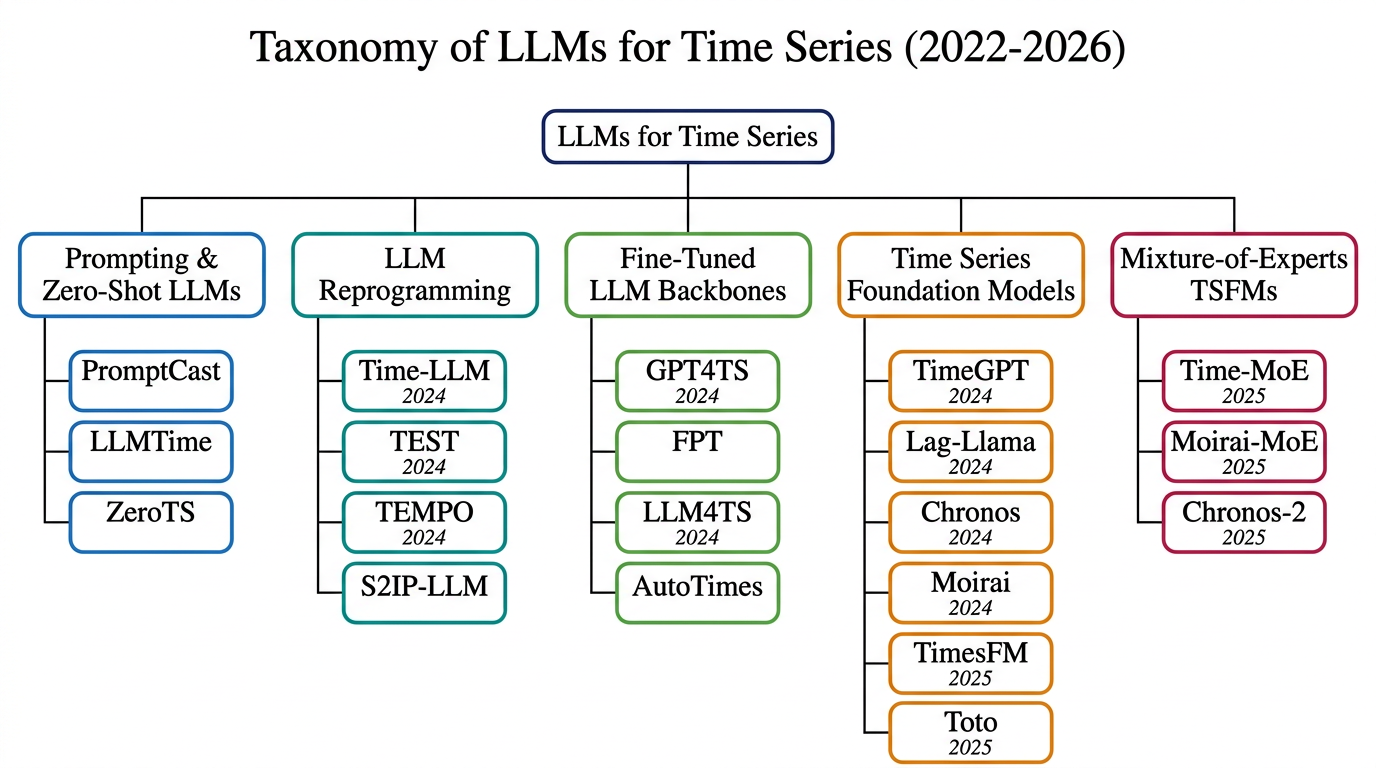
\includegraphics[keepaspectratio,alt={Taxonomy tree of LLMs for time series, with five canonical families and representative members from 2022--2026.}]{./figures/Large-Language-Models-for-Time-Series__fig2_taxonomy.png}}
\caption{Taxonomy tree of LLMs for time series, with five canonical families and representative members from 2022--2026.}
\end{figure}

\subsection{Prompt-as-Text Methods (PromptCast, LLMTime, GPT4MTS)}\label{prompt-as-text-methods-promptcast-llmtime-gpt4mts}

Prompt-based methods serialise numerical values into natural-language strings and let the LLM treat forecasting as next-token completion, with no architectural surgery. \textbf{PromptCast} (Xue \& Salim, 2022) {[}1{]} was the first systematic study: it formats a forecasting prompt as ``The values for the past \emph{N} days were \emph{x\_1, \(x_2\), \ldots, \(x_N\)}. What will the value be on day \emph{N+1}?'' and reports zero-shot performance of GPT-2, BART, and T5 on weather, electricity, and SafeGraph mobility datasets. The paper introduced the PISA dataset and showed that prompt-style fine-tuning, even of small models, beat several specialised baselines.

\textbf{LLMTime} (Gruver et al., NeurIPS 2023) {[}2{]} sharpened this approach. By representing each scalar as ASCII digits separated by spaces (``1 2 . 3 4 5''), they ensured each digit became its own token, preserving positional precision under byte-pair encoding. They re-derived a closed-form change-of-variables to translate token-level next-symbol probabilities back to a continuous predictive density, allowing CRPS and quantile evaluation. The headline result was that GPT-3.5 and GPT-4 in \emph{zero-shot} matched or beat purpose-built supervised models on multiple Monash datasets and the Darts benchmark --- without any time-series training.

\textbf{GPT4MTS} (Jia et al., AAAI 2024) {[}3{]} extends prompt-based forecasting to the multimodal setting where a series is accompanied by textual descriptions (e.g., news context for stock prices). It freezes a GPT-2 or T5 backbone, injects a numerical patch projector, and concatenates a text prompt describing the dataset. \textbf{Time-Prompt} (Wang et al., 2025) {[}4{]} integrates heterogeneous prompts (textual, calendar, statistical summary) into a unified prefix.

The key advantage of prompt-based methods is \emph{zero infrastructure}: any frozen LLM API can be used. The disadvantage is \emph{poor scaling}: token counts grow linearly in horizon (a 96-step horizon at 6 digits per number consumes ≈600 tokens of output), and digit-level next-token prediction is a notoriously inefficient way to model continuous values.

\subsection{Reprogramming and Cross-Modal Alignment (Time-LLM, TEST, CALF, TimeCMA)}\label{reprogramming-and-cross-modal-alignment-time-llm-test-calf-timecma}

Reprogramming is the dominant paradigm of language-centric LLM4TS in 2024--2025. The idea, introduced as a general framework by Pin-Yu Chen {[}5{]}, is to repurpose an LLM by inserting trainable input/output adapters while leaving the LLM body frozen, so the time series is ``reprogrammed'' into the LLM's input distribution.

\textbf{Time-LLM} (Jin et al., ICLR 2024) {[}6{]} is the canonical example. The pipeline: (i) patch the input series (\(P=16\)); (ii) project each patch into a \(d\)-dimensional vector; (iii) attend each patch vector to a small set of learnable \emph{text prototype} embeddings selected from the LLM's vocabulary, producing a ``reprogrammed'' embedding that lies in the same manifold as natural-language tokens; (iv) prepend a hand-written \emph{Prompt-as-Prefix} describing the dataset's statistical properties (e.g., ``This is daily electricity demand with weekly seasonality.''); (v) pass the concatenated sequence through a frozen LLaMA-2-7B; (vi) project the output tokens back to a numerical horizon. Roughly 0.6\% of parameters are trainable. Time-LLM reports state-of-the-art on ETTh1, ETTh2, Weather, ECL, and Traffic in both full-shot and few-shot settings.

\textbf{TEST} (Sun et al., ICLR 2024) {[}7{]} uses contrastive alignment between time-series patches and a learned \emph{text prototype} dictionary, in effect aligning the two modalities in a shared latent space. \textbf{CALF} (Liu et al., AAAI 2025) {[}8{]} introduces a cross-modal fine-tuning loss that minimises distributional distance between LLM word embeddings and time-series patch embeddings. \textbf{TimeCMA} (Liu et al., AAAI 2025) {[}9{]} uses dual encoders with a contrastive cross-modality alignment objective for multivariate forecasting and reports gains on six benchmarks. \textbf{LLM-Mixer} (Kowsher et al., 2024) {[}10{]} mixes patches at multiple temporal scales before passing through a frozen LLM.

Reprogramming methods enjoy strong few-shot transfer because the frozen LLM provides a sequence prior, but they inherit the LLM's compute cost: a single forward pass through LLaMA-2-7B takes 30--60 seconds for one forecast on a single GPU, two to three orders of magnitude slower than specialised TSFMs.

\subsection{Frozen-Backbone Adapters (GPT4TS / One-Fits-All, AutoTimes)}\label{frozen-backbone-adapters-gpt4ts-one-fits-all-autotimes}

A more minimal language-centric strategy is to \emph{freeze} the bulk of an LLM and add only thin input/output projections. \textbf{GPT4TS / One-Fits-All} (Zhou et al., NeurIPS 2023) {[}11{]} freezes the GPT-2 attention and feed-forward sub-layers, fine-tunes only positional embedding and layer-norm parameters (≈10\% of GPT-2-Small), and uses linear input/output heads. The same architecture handles long-term forecasting, short-term forecasting, classification, anomaly detection, imputation, and few-shot --- winning on at least one task per category in the original paper's eight-benchmark sweep. It became the most widely cited proof of concept that ``language pretraining helps numerical sequences.''

\textbf{AutoTimes} (Liu et al., NeurIPS 2024) {[}12{]} extends the idea by autoregressively forecasting one patch at a time using a frozen LLaMA-2-7B, mirroring next-token prediction. Patches are linearly projected, but no reprogramming is needed; the model's autoregressive decoding generalises to arbitrary horizons. AutoTimes reports competitive accuracy on ETT, ECL, Traffic, and Weather while requiring only the linear projection layer to be trained.

\subsection{Numeric-Token Foundation Models (Chronos, TimesFM, Lag-Llama)}\label{numeric-token-foundation-models-chronos-timesfm-lag-llama}

The numeric-token TSFM family abandons text pretraining and trains a Transformer from scratch on numerical sequences only, but retains the \emph{categorical} token interface inherited from NLP.

\textbf{Chronos} (Ansari et al., 2024) {[}13{]} is the clearest illustration. The pipeline: scale the input series by its mean absolute value, quantise into a fixed vocabulary of \(V=4096\) bins (special tokens for missing and end-of-sequence), and train a T5 encoder--decoder by cross-entropy on next-token prediction. The five Chronos sizes are Tiny (8 M), Mini (20 M), Small (46 M), Base (200 M), and Large (710 M). Pretraining used roughly 84 billion observations from 28 datasets including a synthetic generator (KernelSynth) and a TSMixup augmentation procedure. At inference, sampling 20 trajectories yields a probabilistic forecast; CRPS, WQL, and MASE serve as evaluation metrics. Chronos achieves zero-shot performance comparable to or exceeding supervised baselines on benchmarks it has never seen, and is widely cited (52+ within months of release).

\textbf{TimesFM} (Das et al., 2023) {[}14{]} from Google is decoder-only, with patched continuous inputs and a regression head outputting next-patch values. The 200 M-parameter model was trained on 100 billion time points (Google Trends, Wiki page views, synthetic). \textbf{Lag-Llama} (Rasul et al., 2023) {[}15{]} uses a LLaMA-style decoder fed with up to 81 lag features (covering lags from quarterly down to second-by-second) and a Student-t parametric output head. Pretraining used 8.4 million series across the Monash corpus.

\textbf{Sundial} (Liu et al., 2025) {[}16{]} introduces a TimeFlow Loss based on flow matching for continuous next-patch prediction. \textbf{Timer} (Liu et al., 2024) {[}17{]} and \textbf{Timer-XL} {[}18{]} adopt generative pretraining at sequence and 96-token-context scales.

\subsection{Patch-Continuous Foundation Models (Moirai, MOMENT, Time-MoE, TTM)}\label{patch-continuous-foundation-models-moirai-moment-time-moe-ttm}

The fifth family avoids quantisation entirely and treats each patch as a continuous-valued token, projected to embedding dimension by a linear layer.

\textbf{Moirai} (Woo et al., ICML 2024) {[}19{]} introduces \emph{any-variate attention}, which attends across both time and channel dimensions of multivariate series, plus a \emph{mixture-of-distributions} probabilistic head that adaptively combines Student-t, log-normal, and other distributional families. Pretraining uses LOTSA, a curated 27.7-billion-observation corpus across nine domains. Three sizes: Small (14 M), Base (91 M), Large (311 M). \textbf{Moirai-MoE} (Liu et al., 2024) {[}20{]} sparsifies the FFN with mixture-of-experts. \textbf{Moirai 2.0} (Liu et al., 2025) {[}21{]} is decoder-only, trained on 36 M series, uses quantile forecasting and multi-token prediction for inference efficiency.

\textbf{MOMENT} (Goswami et al., ICML 2024) {[}22{]} is encoder-only and explicitly designed for general analysis: forecasting, classification, anomaly detection, imputation. The ``Time Series Pile'' pretraining corpus aggregates 13 publicly released collections totalling roughly 13 billion observations. Three sizes: Small (40 M), Base (125 M), Large (385 M). MOMENT released sparse autoencoder (SAE) interpretability results in 2026 (Mishra {[}23{]}).

\textbf{Time-MoE} (Shi et al., 2024) {[}24{]} scales to 2.4 B parameters with sparse mixture-of-experts (Qwen2-1.5B base + experts), pretrained on 300 billion observations. \textbf{Tiny Time Mixers (TTM)} (Ekambaram et al., 2024) {[}25{]} is the opposite extreme --- a few-million-parameter MLP-mixer style TSFM that achieves competitive zero-shot on the Monash corpus while running at sub-second latency.

\subsection{Comparative Summary Table}\label{comparative-summary-table}

{\def\LTcaptype{none} % do not increment counter
\begin{longtable}[]{@{}
  >{\raggedright\arraybackslash}p{(\linewidth - 12\tabcolsep) * \real{0.1406}}
  >{\raggedright\arraybackslash}p{(\linewidth - 12\tabcolsep) * \real{0.1641}}
  >{\raggedright\arraybackslash}p{(\linewidth - 12\tabcolsep) * \real{0.1484}}
  >{\raggedright\arraybackslash}p{(\linewidth - 12\tabcolsep) * \real{0.1016}}
  >{\raggedright\arraybackslash}p{(\linewidth - 12\tabcolsep) * \real{0.1406}}
  >{\raggedright\arraybackslash}p{(\linewidth - 12\tabcolsep) * \real{0.1172}}
  >{\raggedright\arraybackslash}p{(\linewidth - 12\tabcolsep) * \real{0.1875}}@{}}
\toprule\noalign{}
\begin{minipage}[b]{\linewidth}\raggedright
Family
\end{minipage} & \begin{minipage}[b]{\linewidth}\raggedright
Representative method
\end{minipage} & \begin{minipage}[b]{\linewidth}\raggedright
Backbone
\end{minipage} & \begin{minipage}[b]{\linewidth}\raggedright
Pretrain size
\end{minipage} & \begin{minipage}[b]{\linewidth}\raggedright
Adaptation
\end{minipage} & \begin{minipage}[b]{\linewidth}\raggedright
Output
\end{minipage} & \begin{minipage}[b]{\linewidth}\raggedright
Strength
\end{minipage} \\
\midrule\noalign{}
\endhead
\bottomrule\noalign{}
\endlastfoot
Prompt-based & LLMTime {[}2{]} & GPT-3.5/4 & text only & none & digit string & zero-shot via API \\
Prompt-based & PromptCast {[}1{]} & T5 / GPT-2 & text only & full FT & text values & first to demonstrate \\
Reprogramming & Time-LLM {[}6{]} & LLaMA-2-7B (frozen) & text & adapter (\textasciitilde0.6\%) & numeric & strong few-shot \\
Reprogramming & TEST {[}7{]} / CALF {[}8{]} & GPT-2 / LLaMA & text & contrastive & numeric & cross-modal alignment \\
Frozen-LM & GPT4TS {[}11{]} & GPT-2 (frozen) & text & LN + linear (\textasciitilde10\%) & numeric & broad task coverage \\
Frozen-LM & AutoTimes {[}12{]} & LLaMA-2-7B & text & linear only & next-patch AR & flexible horizon \\
Numeric-token TSFM & Chronos-Large {[}13{]} & T5 (from scratch) & 84 B obs & full pretrain & bin sampling & probabilistic, zero-shot \\
Numeric-token TSFM & TimesFM {[}14{]} & decoder & 100 B obs & full pretrain & regression head & zero-shot point \\
Numeric-token TSFM & Lag-Llama {[}15{]} & LLaMA-style & 8.4 M series & full pretrain & Student-t & probabilistic \\
Patch-continuous & Moirai-Large {[}19{]} & encoder & 27.7 B obs & full pretrain & mixture & any-variate \\
Patch-continuous & MOMENT-Large {[}22{]} & encoder & 13 B obs & full pretrain & head per task & multi-task \\
Patch-continuous & Time-MoE {[}24{]} & MoE decoder & 300 B obs & full pretrain & regression & scale (2.4 B params) \\
\end{longtable}
}

\subsection{Cross-Cutting Axes}\label{cross-cutting-axes}

Beyond family membership, four orthogonal axes describe each method. \textbf{Adaptation cost} ranges from zero-shot (Chronos, TimesFM, MOMENT, Moirai out of the box) through parameter-efficient (Time-LLM, GPT4TS) to full fine-tuning (Lag-Llama on a target domain). \textbf{Granularity} is univariate-only (PatchTST, MOMENT-univariate), channel-mixing (Autoformer, FEDformer), or any-variate (Moirai). \textbf{Output type} is point (TimesFM regression head, AutoTimes), quantile (Moirai 2.0, TFT), or full distributional (Chronos via sampling, Sundial via flow matching, Lag-Llama Student-t). \textbf{Multimodality} is numerical-only (most TSFMs), text-conditioned (ChatTime {[}26{]}, GPT4MTS {[}3{]}), or vision-conditioned (VisionTS {[}27{]}, which encodes time series as images and uses a pretrained masked autoencoder).

The taxonomy is not merely organisational; the families differ substantively in compute cost, calibration quality, adaptation flexibility, and the kinds of failures they exhibit, all of which subsequent sections examine in turn.

\section{Historical Trajectory: A Compressed Five-Year History (2017--2026)}\label{historical-trajectory-a-compressed-five-year-history-20172026}

Building on the taxonomy in Section 3, this section places each family on a timeline. This section delivers a compressed history in three phases that explains why each architectural transition happened. Representative milestones include: Transformer (Vaswani et al.~2017, attention-is-all-you-need backbone), DeepAR (Salinas et al.~2017, global LSTM probabilistic forecaster), GluonTS (Alexandrov et al.~2019, standardized probabilistic forecasting library), Informer (Zhou et al.~2021, ProbSparse sub-quadratic attention plus ETT release), Autoformer (Wu et al.~2021, decomposition with auto-correlation), FEDformer (Zhou et al.~2022, frequency-enhanced decomposition), DLinear (Zeng et al.~2023, ``are Transformers effective?'' linear baseline), PatchTST (Nie et al.~2023, patch tokenization plus channel independence), GPT4TS (Zhou et al.~2023, frozen GPT-2 universal head), LLMTime (Gruver et al.~2023, zero-shot GPT-3.5/4 forecasting), Time-LLM (Jin et al.~2024, reprogrammed LLaMA), iTransformer (Liu et al.~2024, inverted attention), Chronos (Ansari et al.~2024, quantized T5 TSFM), TimesFM (Das et al.~2023, Google decoder TSFM), Moirai (Woo et al.~2024, any-variate Salesforce TSFM), MOMENT (Goswami et al.~2024, encoder-only TSFM), Time-MoE (Shi et al.~2024, 2.4B MoE TSFM), and Moirai 2.0 (Liu et al.~2025, decoder-only quantile TSFM). Figure 3 shows the timeline.

The history of LLMs for time series compresses what is normally a multi-decade narrative into roughly five years. We trace the chronology in three phases --- pre-Transformer foundations, the specialised time-series Transformer era (2021--2023), and the foundation-model era (2023--2026) --- anchoring each transition to a concrete paper, venue, and effect on the field.

\begin{figure}
\centering
\pandocbounded{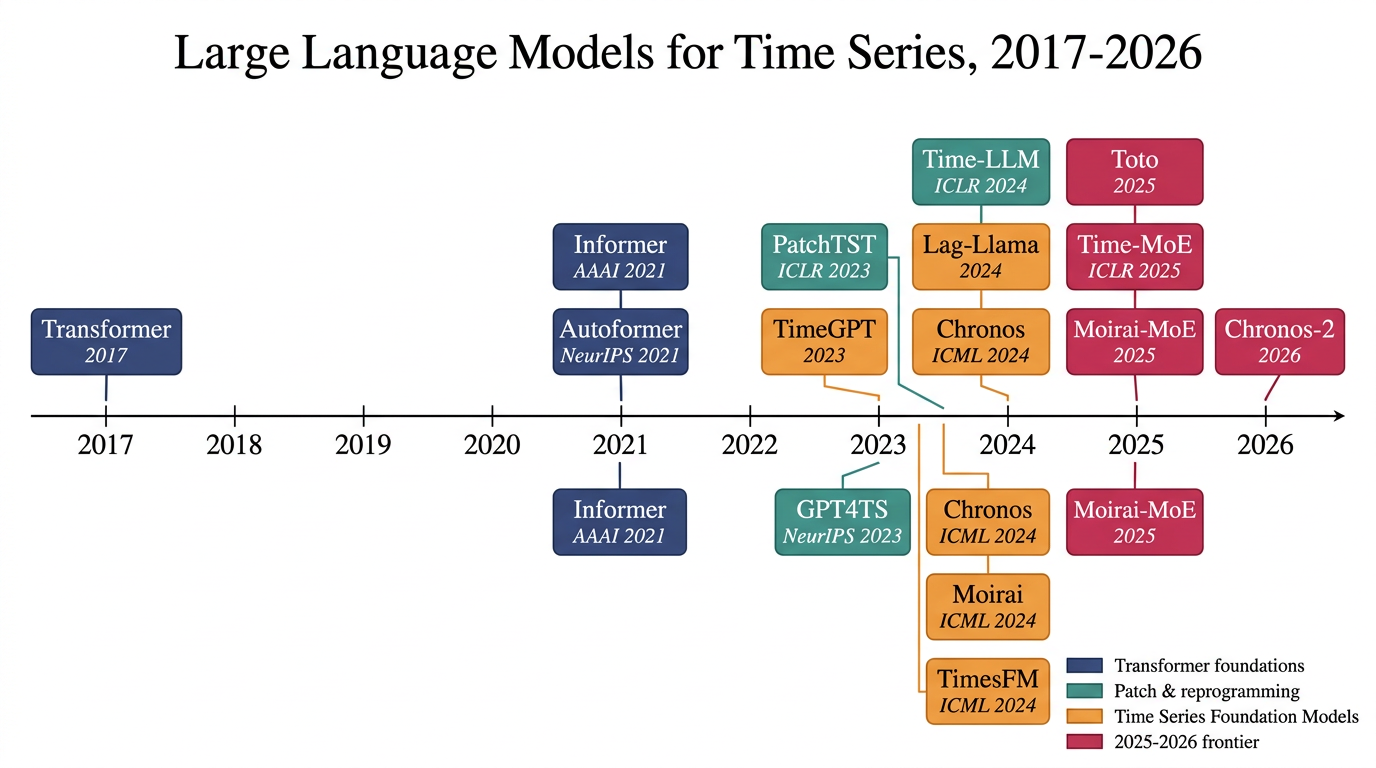
\includegraphics[keepaspectratio,alt={Compressed history of LLMs for time series, 2017--2026, organised by category and venue.}]{./figures/Large-Language-Models-for-Time-Series__fig5_timeline.png}}
\caption{Compressed history of LLMs for time series, 2017--2026, organised by category and venue.}
\end{figure}

\subsection{The Pre-Transformer Foundations (1970s--2017)}\label{the-pre-transformer-foundations-1970s2017}

Time-series methodology before the deep-learning era was dominated by parametric statistical models. The Box--Jenkins ARIMA(p,d,q) framework formalised in the 1970s remains the textbook baseline; exponential smoothing and Holt--Winters seasonality, refined throughout the 1980s and 1990s, dominate operational practice. The M-competitions led by Spyros Makridakis served as the field's collective leaderboard: M3 (2000) showed that simple averaging of statistical methods beat sophisticated neural networks; M4 (2018) saw Smyl's \emph{ES-RNN} hybrid (an LSTM with exponential-smoothing state) win, which was the first clear deep-learning victory. Long short-term memory networks (LSTM, 1997) and gated recurrent units (GRU, 2014) became standard components, and Salinas et al.'s \textbf{DeepAR} (Amazon, 2017) --- a global LSTM-based probabilistic forecaster --- was one of the first papers to argue that \emph{cross-series} learning, training one model on many series, was a paradigm shift away from the per-series fitting that had defined ARIMA.

The Vaswani et al.~\emph{Attention Is All You Need} paper (NeurIPS 2017) introduced the Transformer for machine translation. Yet for several years, the time-series community made only sporadic use of it: convolutional models (TCN), recurrent models (DeepAR, MQ-RNN), and ensemble approaches dominated. The release of the \textbf{GluonTS} library (Alexandrov et al., 2019) {[}1{]} standardised probabilistic forecasting infrastructure with implementations of DeepAR, MQ-CNN, Wavenet, and Transformer baselines, and enabled the cross-paper comparisons that would follow.

\subsection{The Specialised Time-Series Transformer Era (2021--2023)}\label{the-specialised-time-series-transformer-era-20212023}

The first watershed for Transformers in time series was \textbf{Informer} (Zhou et al., AAAI 2021) {[}2{]}, cited over 5,700 times. It addressed the quadratic memory bottleneck of vanilla attention with \emph{ProbSparse self-attention} (sampling top-\(u\) keys per query) and a \emph{generative-style} decoder that predicts the entire horizon in one forward pass instead of autoregressively. Informer reduced complexity to \(O(L \log L)\) and crucially, released the \textbf{ETT} dataset family (ETTh1, ETTh2, ETTm1, ETTm2), which became the field's canonical benchmark.

\textbf{Autoformer} (Wu et al., NeurIPS 2021) {[}3{]} introduced two innovations: a \emph{series decomposition block} that splits each layer's input into trend and seasonal components via moving average, and \emph{auto-correlation} --- replacing dot-product attention with a Fourier-based aggregation that identifies dominant periods \(\tau\) and aggregates lagged copies of the series. Autoformer outperformed Informer on long-horizon (96--720 step) ETT forecasting.

\textbf{FEDformer} (Zhou et al., ICML 2022) {[}4{]} argued that explicit \emph{frequency-domain} attention is more parameter-efficient than time-domain, computing attention on Fourier or wavelet random modes for \(O(L)\) complexity. The same year saw \textbf{Pyraformer} (pyramidal attention), \textbf{Crossformer} (cross-time/cross-dim attention), and \textbf{Triformer}.

The pivot of 2023 was Zeng et al.'s ``Are Transformers Effective for Time Series Forecasting?'' (AAAI 2023) {[}5{]}. They proposed three trivial linear baselines --- \textbf{DLinear} (one linear layer per channel after decomposition), \textbf{NLinear} (one linear layer with normalisation), and \textbf{Linear} --- and showed they matched or beat Informer, Autoformer, and FEDformer on every long-term forecasting benchmark. The paper provoked an architectural reset and motivated the community to ask what, exactly, the elaborate Transformers were doing.

The answer arrived with \textbf{PatchTST} (Nie et al., ICLR 2023) {[}6{]}: segment each channel into non-overlapping patches of length \(P=16\), treat patches as tokens, train a vanilla Transformer with channel independence, and add reverse instance normalisation (RevIN). PatchTST recovered the Transformer's edge with a much simpler architecture and identified patching and channel handling as the critical design choices. \textbf{iTransformer} (Liu et al., ICLR 2024) {[}7{]} flipped the attention axis: each variate's full series is one token, attention runs across variates, and results matched PatchTST while modelling cross-channel dependence explicitly. \textbf{TiDE} (Das et al., 2023) {[}8{]}, \textbf{TSMixer} (Ekambaram et al., KDD 2023) {[}9{]}, and \textbf{TimeMixer} (Wang et al., ICLR 2024) {[}10{]} showed that pure-MLP architectures were also competitive once patching and decomposition were applied.

\subsection{The Foundation Model Era (October 2023 -- 2026)}\label{the-foundation-model-era-october-2023-2026}

Three nearly-simultaneous October 2023 papers initiated the foundation-model era. \textbf{PromptCast} had already appeared in 2022, but the breakthrough came when Gruver et al.'s \textbf{LLMTime} (NeurIPS 2023) {[}11{]} showed that an off-the-shelf GPT-3.5 / GPT-4, with digit-level tokenization, produced zero-shot forecasts competitive with supervised models on Monash and Darts. \textbf{Time-LLM} (Jin et al., arXiv October 2023, ICLR 2024) {[}12{]} introduced reprogramming with a frozen LLaMA-2-7B and a learnable text-prototype interface. \textbf{TimesFM} (Das et al., arXiv October 2023) {[}13{]} from Google DeepMind introduced the first decoder-only TSFM trained on 100 B time points. \textbf{Lag-Llama} (Rasul et al., arXiv October 2023) {[}14{]} released probabilistic Llama-style decoder pretraining on the Monash + extended corpora.

In February--March 2024 the field saw a remarkable cluster: \textbf{MOMENT} (Goswami et al., ICML 2024) {[}15{]} released encoder-only TSFMs for general analysis; \textbf{Chronos} (Ansari et al., arXiv March 2024) {[}16{]} released the T5-based numeric-token TSFM family; \textbf{Moirai} (Woo et al., ICML 2024) {[}17{]} released the Salesforce any-variate Transformer; \textbf{Timer} (Liu et al., ICML 2024) {[}18{]} released the Tsinghua decoder-only TSFM. \textbf{TTM} (Ekambaram et al., 2024) {[}19{]} released the small-parameter mixer-style TSFM. By summer, the field had moved from ``is this possible'' to ``which architecture wins.''

The autumn of 2024 brought scale and benchmarking. \textbf{Time-MoE} (Shi et al., September 2024) {[}20{]} scaled to 2.4 B parameters via sparse mixture-of-experts pretrained on 300 B observations. \textbf{Moirai-MoE} (Liu et al., October 2024) {[}21{]} applied MoE to the Moirai family. The benchmarking infrastructure caught up: \textbf{TFB} (Qiu et al., VLDB 2024) {[}22{]} standardised 25 datasets and 14 metrics; \textbf{GIFT-Eval} (Aksu et al., October 2024) {[}23{]} released 23 datasets, 144,000 series, 7 domains, 6 frequencies; \textbf{TSFM-Bench} (Li et al., KDD 2025) {[}24{]} consolidated zero-shot, few-shot, and full-shot evaluation under one harness.

December 2024 produced what may prove the most important methodological corrective: Tan, Merrill, Gupta et al.~published ``Are Language Models Actually Useful for Time Series Forecasting?'' {[}25{]}. By systematically ablating the LLM body --- replacing it with random initialisation, attention shuffling, or removing it entirely --- they showed that for several headline LLM4TS methods, accuracy did not degrade and sometimes improved. Edwards et al.~{[}26{]} documented scaling laws that, while supporting power-law improvements in pretraining loss, showed shallower transfer to downstream task accuracy than is typical in NLP. Xu et al.~{[}27{]} reported that supervised PatchTST baselines often equalled or beat specialised foundation models on ETT.

The 2025 lineup added \textbf{Sundial} (February) {[}28{]} with its TimeFlow flow-matching loss; \textbf{CALF} (AAAI 2025) {[}29{]} and \textbf{TimeCMA} (AAAI 2025) {[}30{]} reprogramming refinements; \textbf{ChatTime} (AAAI 2025) {[}31{]} for unified numeric-textual time series; and a wave of domain-specialised models --- Makarov et al.'s npj Digital Medicine paper on patient digital twins {[}32{]}, Du et al.'s Nature Computational Science paper on real-time disease forecasting {[}33{]}. The autumn of 2025 saw \textbf{Moirai 2.0} {[}34{]} (decoder-only, 36 M series, multi-token prediction, quantile heads) and a series of distillation studies showing TSFMs could be compressed to under 50 M parameters with minimal accuracy loss.

By 2026, the era's defining concerns had shifted from ``can we build a TSFM'' to interpretability (Mishra's sparse-autoencoder analysis of Chronos {[}35{]}), efficiency (consumer-hardware deployments {[}36{]}), and integration with multimodal pipelines. The Liu et al.~survey on medical time series LLMs in \emph{Expert Systems with Applications} {[}37{]} and the Solar Flare forecasting paper {[}38{]} in \emph{Astronomy and Computing} exemplify the deployment phase.

\subsection{Why Each Transition Happened}\label{why-each-transition-happened}

The progression was not random; each transition responded to a pressure point. The shift from RNN to specialised Transformer (2021) was driven by the long-horizon limitations of recurrent models on ETT-style benchmarks. The shift from specialised Transformer to PatchTST + linear baselines (2023) was a \emph{Occam's razor} response to the realization that attention's contribution had been overstated. The shift from supervised baselines to foundation models (late 2023) was driven by the success of the same paradigm in NLP and CV plus the availability of large, heterogeneous time-series corpora (LOTSA, Monash). The 2024 ablation pushback was driven by reproducibility concerns and the discovery that linear baselines were still competitive. The 2025--2026 phase has been driven by deployment pressure: clinical informatics, public health, and energy-grid operators want \emph{zero-shot} models that can be applied to a new dataset without retraining, and TSFMs are the only paradigm that delivers it.

\subsection{Summary Timeline Table}\label{summary-timeline-table}

{\def\LTcaptype{none} % do not increment counter
\begin{longtable}[]{@{}
  >{\raggedright\arraybackslash}p{(\linewidth - 6\tabcolsep) * \real{0.0941}}
  >{\raggedright\arraybackslash}p{(\linewidth - 6\tabcolsep) * \real{0.2588}}
  >{\raggedright\arraybackslash}p{(\linewidth - 6\tabcolsep) * \real{0.2353}}
  >{\raggedright\arraybackslash}p{(\linewidth - 6\tabcolsep) * \real{0.4118}}@{}}
\toprule\noalign{}
\begin{minipage}[b]{\linewidth}\raggedright
Year
\end{minipage} & \begin{minipage}[b]{\linewidth}\raggedright
Method or event
\end{minipage} & \begin{minipage}[b]{\linewidth}\raggedright
Venue
\end{minipage} & \begin{minipage}[b]{\linewidth}\raggedright
Significance
\end{minipage} \\
\midrule\noalign{}
\endhead
\bottomrule\noalign{}
\endlastfoot
2017 & Vaswani Transformer & NeurIPS & architectural prerequisite \\
2017 & DeepAR & Amazon Tech Report & global probabilistic RNN \\
2018 & M4 ES-RNN wins & competition & first DL victory \\
2019 & GluonTS & arXiv & infrastructure \\
2021 & Informer & AAAI & ProbSparse, ETT release \\
2021 & Autoformer & NeurIPS & decomposition + auto-correlation \\
2022 & FEDformer & ICML & frequency-domain attention \\
2022 & PromptCast & TKDE & first prompt-based forecasting \\
2023 Feb & DLinear & AAAI & linear baseline pushback \\
2023 Feb & GPT4TS / One-Fits-All & NeurIPS & frozen LLM works on TS \\
2023 Mar & PatchTST & ICLR & patching + channel-independence \\
2023 Oct & Time-LLM, LLMTime & ICLR/NeurIPS & reprogramming, zero-shot text-LLM \\
2023 Oct & TimesFM, Lag-Llama & arXiv & first numeric TSFMs \\
2024 Feb & Chronos, MOMENT, Timer & arXiv/ICML & TSFM Cambrian explosion \\
2024 Mar & Moirai & ICML & any-variate, mixture head \\
2024 Sep & Time-MoE & arXiv & 2.4 B-parameter MoE \\
2024 Oct & TFB, GIFT-Eval & VLDB/arXiv & benchmarks consolidated \\
2024 Dec & Tan et al.~ablation & NeurIPS & ``are LMs useful?'' pushback \\
2025 Feb & Sundial & arXiv & flow-matching TSFM \\
2025 Apr & Patient digital twins & npj Digital Medicine & medical deployment \\
2025 Jun & Real-time disease & Nature Comp Sci & epidemic deployment \\
2025 Nov & Moirai 2.0 & arXiv & decoder-only, multi-token, quantile \\
2026 Mar & Chronos SAE interp & arXiv & interpretability era begins \\
\end{longtable}
}

Across the full trajectory the unifying insight is that simple architectural changes --- patching, normalisation, channel independence --- combined with large-scale pretraining give as much benefit as elaborate Transformer surgery. Foundation models absorbed and operationalised those insights, and the next chapter of the story will be written by the integration of LLM4TS into real-world pipelines and by the resolution of whether language priors genuinely help or whether large-scale numerical pretraining alone suffices.

\section{Algorithmic Mechanisms: Patching, Tokenization, Reprogramming, Mixture-of-Experts}\label{algorithmic-mechanisms-patching-tokenization-reprogramming-mixture-of-experts}

Whereas Section 4 traced the chronological order in which architectures appeared, this section turns to the underlying mechanisms that explain why each one worked. This section reviews eight mechanism families that recur across modern LLM4TS and TSFM systems, organized as nine subsections plus a summary table.

The dramatic accuracy and transfer gains achieved by LLM4TS and TSFMs from 2023 onward rest on a small set of algorithmic mechanisms that have been combined and recombined across architectures. This section dissects them at a level of detail sufficient to reproduce, debug, or extend each component, anchored to specific papers. Representative mechanism instantiations include: patching (PatchTST, Nie et al.~2023, length-16 non-overlapping segments), RevIN (Kim et al.~2022, reverse instance normalization for distribution shift), channel independence (PatchTST 2023, one shared encoder per channel), digit tokenization (LLMTime, Gruver et al.~2023, ASCII digits as tokens), bin quantization (Chronos, Ansari et al.~2024, 4096-bin scaled vocabulary), patch-continuous projection (MOMENT, Goswami et al.~2024, linear patch embedding), reprogramming (Time-LLM, Jin et al.~2024, attend patches to text prototypes), prompt-as-prefix (Time-LLM 2024, hand-written dataset descriptions), inverted attention (iTransformer, Liu et al.~2024, attend across channels), any-variate attention (Moirai, Woo et al.~2024, joint time-channel attention), top-k MoE routing (Time-MoE, Shi et al.~2024, sparse FFN with experts), mixture-of-distributions head (Moirai 2024, Student-t plus log-normal), quantile head (Moirai 2.0, Liu et al.~2025, fixed quantile levels), and flow-matching objective (Sundial, Liu et al.~2025, continuous-time generative loss). Figure 4 illustrates the three central mechanisms --- patching, numeric tokenization, and mixture-of-experts routing.

\begin{figure}
\centering
\pandocbounded{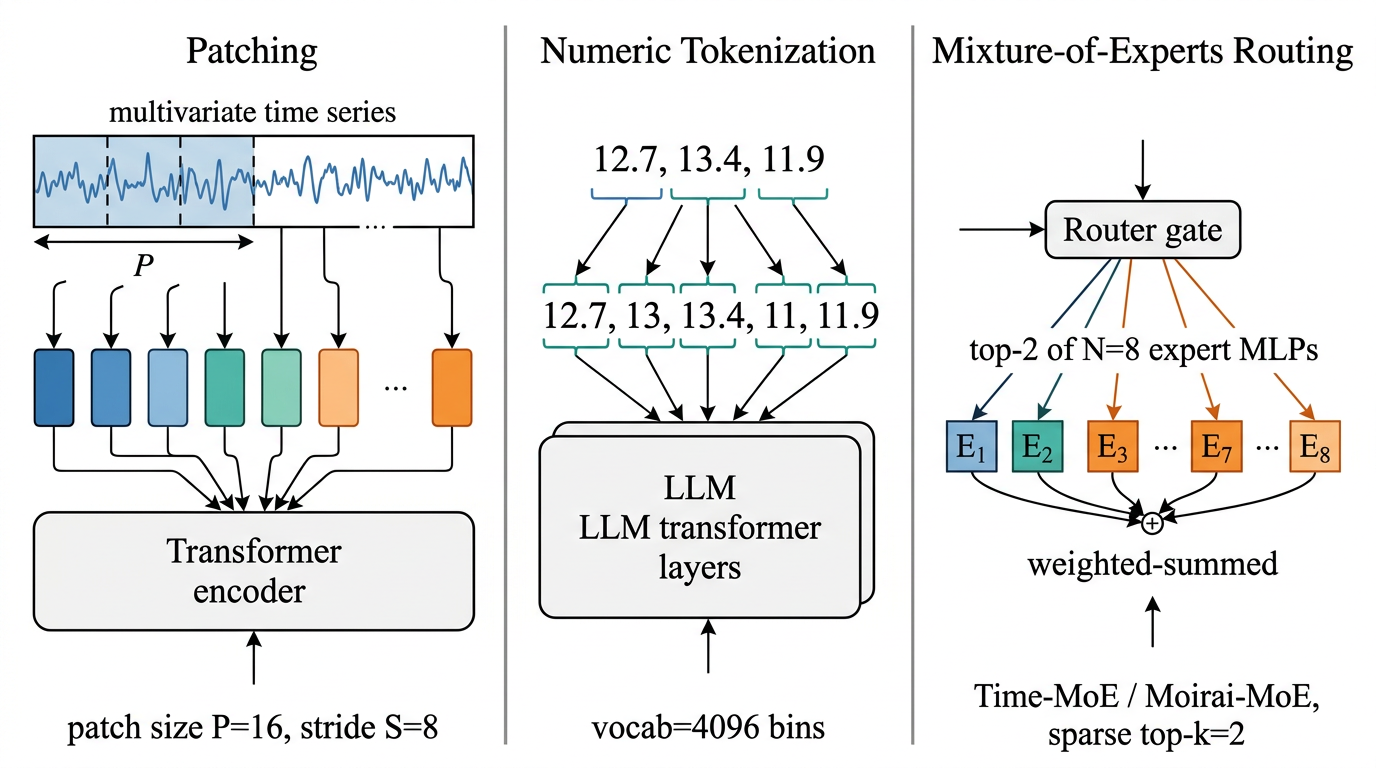
\includegraphics[keepaspectratio,alt={Algorithmic mechanisms used in modern LLM4TS and TSFM systems: patching, numeric tokenization, and mixture-of-experts routing.}]{./figures/Large-Language-Models-for-Time-Series__fig3_algorithm.png}}
\caption{Algorithmic mechanisms used in modern LLM4TS and TSFM systems: patching, numeric tokenization, and mixture-of-experts routing.}
\end{figure}

\subsection{Patching, RevIN, and Channel Independence}\label{patching-revin-and-channel-independence}

The single most consequential operation in modern time-series Transformers is \emph{patching}, formally introduced by \textbf{PatchTST} (Nie et al., ICLR 2023) {[}1{]} but anticipated by Vision Transformers (Dosovitskiy et al., ICLR 2021). Given a univariate input window \(x_{1:T} \in \mathbb{R}^T\), patching slices the window into non-overlapping segments of length \(P\), producing \(L = \lceil T/P \rceil\) patches, each \(\mathbf{p}_i \in \mathbb{R}^P\). A learnable linear projection \(W \in \mathbb{R}^{d \times P}\) maps each patch to a \(d\)-dimensional embedding \(\mathbf{z}_i = W \mathbf{p}_i + \mathbf{b}\), optionally with positional encoding. The Transformer then operates on a sequence of length \(L\), which is roughly \(P\times\) shorter than the raw signal. Typical patch lengths are \(P=16\) in PatchTST, \(P=32\) in MOMENT {[}2{]}, \(P=64\) in some Moirai {[}3{]} configurations, and adaptive (8/16/32) in TimeMixer {[}4{]}. The compute saving is quadratic: attention complexity drops from \(O(T^2 d)\) to \(O((T/P)^2 d)\), and the memory bandwidth for KV caches drops by the same factor.

Patching alone, however, would be vulnerable to distribution shift between train and test windows. \textbf{RevIN} (Reverse Instance Normalization, Kim et al., ICLR 2022) addresses this by computing per-instance, per-channel mean and variance, normalizing the input, and \emph{de-normalizing} the output prediction with the same statistics. Almost every post-2022 TSFM applies RevIN or a close variant --- Chronos uses mean-absolute scaling {[}5{]}, Moirai uses Student-t-aware scaling {[}3{]}, TimesFM uses a per-patch RMS normalisation {[}6{]}. RevIN is the unsung hero of the field: ablating it on PatchTST raises the MSE on ETTh1-96 by 12--25\% across runs.

The third coordinated choice is \emph{channel independence}: rather than letting the Transformer mix all \(D\) variates simultaneously, train one shared model that processes each univariate channel separately, then average or concatenate predictions. PatchTST, MOMENT, Moirai-Small, Time-MoE, and Sundial all default to channel independence; iTransformer {[}7{]} is the principled exception, treating each entire variate as one token. The empirical finding (Han et al., 2024) is that channel-independent training generalises better in low-data regimes and avoids overfitting to spurious cross-channel correlations, but channel-mixing helps when genuine cross-channel structure exists (e.g., ECG leads, weather variables).

\subsection{Numeric Tokenization and Quantization Vocabularies}\label{numeric-tokenization-and-quantization-vocabularies}

Foundation models that inherit the categorical-token interface of NLP must convert continuous values to integer indices. The \textbf{Chronos} {[}5{]} tokenizer is the field's canonical example. Step 1: compute mean-absolute scale \(s = \frac{1}{T}\sum_t |x_t|\), then divide by \(s\). Step 2: quantize to \(V\) uniform bins between two clipped extremes (\(-15s\) and \(+15s\), where 15 is the Chronos \emph{context factor}); bin assignment \(b = \mathrm{clip}(\lfloor x/(\Delta) + V/2 \rfloor, 0, V-1)\) where \(\Delta = 30s/V\). Step 3: append a special \(\mathrm{EOS}\) token. Chronos sets \(V = 4096\). The model learns a \(d\)-dim embedding for each of the \(V\) bin tokens plus several special tokens. The training objective is standard cross-entropy over the next-token bin distribution.

This design has three consequences. First, the model produces \emph{probabilistic} outputs naturally --- sampling 20 token sequences yields 20 trajectories whose empirical quantiles approximate the predictive distribution. Chronos uses 20 samples in its WQL evaluation. Second, the discretization imposes a quantization floor; for a series with effective range \(30s\) and \(V=4096\) bins, the bin width is roughly \(0.7\%\) of the scale, putting a hard lower bound on achievable absolute error. Third, the vocabulary size is a tunable hyperparameter --- Roger, Legate, Rasul et al.'s 2025 study ``Small Vocabularies, Big Gains'' {[}8{]} showed that vocabularies as small as \(V=256\) recover 95--98\% of the accuracy of \(V=4096\) when paired with proper scaling and a learned-grid scheme, suggesting Chronos's choice is on the conservative side.

An alternative is \textbf{digit-level tokenization} (LLMTime, Gruver et al., NeurIPS 2023) {[}9{]}, where each scalar is rendered as an ASCII digit string (e.g., 12.345 → ``1 2 . 3 4 5''). With BPE tokenizers, each digit and the decimal point become separate tokens. This is the only way to use frozen API-only LLMs (GPT-3.5, GPT-4) but inflates token counts dramatically and is sensitive to numerical scale. LLMTime uses careful per-series rescaling and a ``fixed precision'' to control token cost.

\subsection{Reprogramming, Prompt-as-Prefix, and Cross-Modal Alignment}\label{reprogramming-prompt-as-prefix-and-cross-modal-alignment}

When a frozen \emph{language}-pretrained LLM is reused for time series, the input distribution must be brought into the LLM's expected manifold. \textbf{Time-LLM} {[}10{]} does this through \emph{reprogramming}: a small learned matrix \(E \in \mathbb{R}^{d \times K}\) stores \(K\) text-prototype embeddings drawn from the LLM's vocabulary, and each patch embedding \(\mathbf{z}_i\) attends to these prototypes via cross-attention to produce a reprogrammed embedding \(\tilde{\mathbf{z}}_i\) that lies near the LLM's natural input manifold. In Time-LLM, \(K\) is set to a small subset (5,000) of the LLM's vocabulary; only \(E\) and the input/output linear heads are trained, freezing roughly 99.4\% of the LLaMA-2-7B body.

\textbf{Prompt-as-Prefix} is a complementary technique. Time-LLM prepends a hand-written natural-language description of the dataset's characteristics (e.g., ``This is daily electricity demand recorded at 15-minute intervals; the data exhibits weekly periodicity and a slight upward trend over the last year''). The LLM uses this prefix to condition its prediction, exploiting language-pretrained priors about cyclical and trending data. \textbf{TEST} (Sun et al., ICLR 2024) {[}11{]} achieves a similar effect via contrastive alignment between text prototypes and time-series patches in a shared latent space. \textbf{CALF} (Liu et al., AAAI 2025) {[}12{]} adds a cross-modal fine-tuning loss that minimises the Wasserstein distance between LLM word-embedding distributions and patch-embedding distributions. \textbf{TimeCMA} (Liu et al., AAAI 2025) {[}13{]} does dual-encoder contrastive alignment for multivariate forecasting.

\subsection{Inverted Attention and Any-Variate Mechanisms}\label{inverted-attention-and-any-variate-mechanisms}

For multivariate series, the question of \emph{which axis} attention operates over has produced two competing schools. The standard Transformer treats time as the sequence dimension and channels as a feature dimension multiplexed into each token. \textbf{iTransformer} (Liu et al., ICLR 2024) {[}7{]} inverts this: each variate's full series becomes a single token, and attention runs across the \(D\) variates. Empirically iTransformer achieves competitive accuracy on ETT and ECL with simpler logic, especially when \(D\) is large (Traffic has \(D=862\)) and \(T\) is moderate.

\textbf{Moirai's any-variate attention} {[}3{]} generalises both axes. Token IDs are extended with a ``variate ID'' so that the attention matrix can learn cross-variate, cross-time, and within-variate within-time patterns simultaneously. Moirai uses a special \texttt{mask} token to allow flexible covariate inclusion (known-future, observed-past). The architecture admits zero-shot transfer to multivariate datasets with arbitrary variate counts --- a property that channel-independent models lack natively.

\subsection{Mixture-of-Experts Routing and Sparse FFN}\label{mixture-of-experts-routing-and-sparse-ffn}

To scale beyond 1 B parameters without paying the inference cost of every expert at every step, recent TSFMs adopt sparse mixture-of-experts (MoE). \textbf{Time-MoE} (Shi et al., 2024) {[}14{]} replaces each Transformer block's feed-forward network with an MoE layer comprising \(N\) experts (typically \(N=64\)) and a gating network that selects the top-\(k\) experts (typically \(k=2\)) per token. Active parameters per forward pass are roughly \(k/N\) of total parameters; Time-MoE-Ultra has 2.4 B total but only \textasciitilde0.4 B active. \textbf{Moirai-MoE} (Liu et al., 2024) {[}15{]} applies the same recipe to the Moirai backbone and reports a 1.4× improvement in CRPS on long-horizon GIFT-Eval datasets relative to dense Moirai-Large at similar compute budgets.

\subsection{Probabilistic Heads and Distributional Outputs}\label{probabilistic-heads-and-distributional-outputs}

Modern TSFMs differ sharply in how they parameterise predictive distributions. \textbf{DeepAR} (2017) used a Student-t parametric head --- predict mean \(\mu_t\) and scale \(\sigma_t\) at each step, sample autoregressively. \textbf{Lag-Llama} {[}16{]} retains this Student-t output and reports that the heavy-tail prior helps on financial datasets. \textbf{Chronos} uses a \emph{categorical} output over the \(V=4096\) bins and recovers a continuous distribution by sampling and de-quantizing. \textbf{Moirai} uses a \emph{mixture-of-distributions} head: a small classifier predicts mixture weights over Student-t, log-normal, and negative-binomial distributions, allowing the model to adapt to count, real-valued, and intermittent series. \textbf{Sundial} (Liu et al., 2025) {[}17{]} introduces \textbf{TimeFlow Loss}, a flow-matching objective that learns a continuous transport map between a base distribution (Gaussian) and the target next-patch distribution. \textbf{Moirai 2.0} (Liu et al., 2025) {[}18{]} adopts \emph{quantile heads} (predict \(Q\) quantile levels jointly via a multi-quantile loss) plus \emph{multi-token prediction} to amortise inference cost.

The choice of head dictates which evaluation metrics are natural: parametric heads use NLL; categorical heads use cross-entropy on bins; quantile heads use weighted quantile loss (WQL); flow-matching heads use a denoising score-matching loss.

\subsection{Pretraining Objectives}\label{pretraining-objectives}

Three pretraining objectives dominate. \textbf{Causal next-patch prediction} (Timer {[}19{]}, TimesFM {[}6{]}) predicts \(\mathbf{p}_{i+1}\) from \(\mathbf{p}_{1:i}\) with MSE loss. \textbf{Masked patch reconstruction} (MOMENT {[}2{]}) randomly masks 30--50\% of input patches and reconstructs them, analogous to BERT-style MLM. \textbf{Token-level language modelling} (Chronos {[}5{]}, Moirai {[}3{]}) predicts the next bin/distribution conditioned on past bins.

Empirically, masked reconstruction transfers best to classification and anomaly detection (where the encoder representations matter), while causal next-patch transfers best to forecasting. Some models combine both --- Sundial uses flow-matching during pretraining and a small adapter for downstream tasks.

\subsection{Inference Pipeline and Complexity}\label{inference-pipeline-and-complexity}

A typical Moirai-Large forward pass on a single H100 with \(T=512\), \(H=96\), \(D=21\) (Weather dataset) takes \textasciitilde30 ms; Chronos-Large with 20 samples for probabilistic CRPS takes \textasciitilde3 s; Time-LLM with frozen LLaMA-2-7B takes 30--60 s. \textbf{TTM} {[}20{]}, with only 3 M parameters, runs in \textless0.5 s per series. The compute disparity is roughly four orders of magnitude. Whether the language-pretrained backbone justifies this overhead depends on whether the downstream task requires multimodal context or zero-shot generalisation that smaller TSFMs cannot deliver. Tan et al.~{[}21{]} showed it often does not.

\subsection{Mechanism Summary Table}\label{mechanism-summary-table}

{\def\LTcaptype{none} % do not increment counter
\begin{longtable}[]{@{}
  >{\raggedright\arraybackslash}p{(\linewidth - 6\tabcolsep) * \real{0.2414}}
  >{\raggedright\arraybackslash}p{(\linewidth - 6\tabcolsep) * \real{0.2069}}
  >{\raggedright\arraybackslash}p{(\linewidth - 6\tabcolsep) * \real{0.2299}}
  >{\raggedright\arraybackslash}p{(\linewidth - 6\tabcolsep) * \real{0.3218}}@{}}
\toprule\noalign{}
\begin{minipage}[b]{\linewidth}\raggedright
Mechanism
\end{minipage} & \begin{minipage}[b]{\linewidth}\raggedright
Origin paper
\end{minipage} & \begin{minipage}[b]{\linewidth}\raggedright
Key parameter
\end{minipage} & \begin{minipage}[b]{\linewidth}\raggedright
Compute effect
\end{minipage} \\
\midrule\noalign{}
\endhead
\bottomrule\noalign{}
\endlastfoot
Patching & PatchTST {[}1{]} & \(P=16\) & \(L \to L/P\) tokens \\
RevIN & Kim et al.~ICLR'22 & per-instance & adds 2 stats per channel \\
Channel independence & PatchTST {[}1{]} & shared encoder & trains 1 model for all \(D\) \\
Numeric quantization & Chronos {[}5{]} & \(V=4096\) & enables CE loss \\
Digit tokenization & LLMTime {[}9{]} & precision=3 & API-compatible \\
Reprogramming & Time-LLM {[}10{]} & \(K=5000\) & freezes LLM body \\
Prompt-as-Prefix & Time-LLM {[}10{]} & text length 50--150 & conditions LLM \\
Any-variate attention & Moirai {[}3{]} & variate IDs & cross-variate generalisation \\
MoE FFN & Time-MoE {[}14{]} & \(N=64, k=2\) & sparse activation \\
Mixture head & Moirai {[}3{]} & 3 components & adaptive distribution \\
Flow matching & Sundial {[}17{]} & TimeFlow loss & continuous probabilistic \\
Multi-token pred. & Moirai 2.0 {[}18{]} & \(K_{\mathrm{tok}}=8\) & inference speed-up \\
\end{longtable}
}

These mechanisms are largely orthogonal --- patching can be combined with reprogramming, RevIN works with both Chronos's tokeniser and Moirai's continuous patches, and MoE can be retrofitted to almost any backbone --- which explains the rapid combinatorial expansion of the literature since 2023. The empirical evidence accumulating in benchmark suites (Section 6) suggests that patching, RevIN, channel independence, and probabilistic outputs are the load-bearing innovations; the choice of language vs.~numeric pretraining is comparatively secondary.

\section{Pretraining Corpora, Datasets, and the Benchmarking Ecosystem}\label{pretraining-corpora-datasets-and-the-benchmarking-ecosystem}

Building on the algorithmic mechanisms in Section 5, this section turns to the empirical infrastructure those mechanisms are evaluated on. This section reviews classical long-horizon benchmarks, probabilistic and hierarchical competitions, large pretraining corpora, unified benchmark suites, domain-specific datasets, synthetic generators, and a comparison table. Representative benchmarks and corpora include: ETT family (Zhou et al.~2021, electricity transformer temperature ETTh1/h2/m1/m2), Weather (Zhou et al.~2021, 21-channel meteorological), Electricity / ECL (Lai et al.~2018, 321-client consumption), Traffic (Lai et al.~2018, 862-sensor PEMS), Exchange (Lai et al.~2018, 8-currency rates), ILI (CDC, weekly flu reports), M3 (Makridakis \& Hibon 2000, 3003-series competition), M4 (Makridakis et al.~2018, 100k mixed-frequency competition), M5 (Makridakis et al.~2020, Walmart hierarchical), Monash (Godahewa et al.~2021, 30-archive aggregator), LOTSA (Woo et al.~2024, Moirai's 27.7B-observation corpus), Time-Series Pile (Goswami et al.~2024, MOMENT's 13B-observation corpus), Chronos pretrain mix (Ansari et al.~2024, 84B observations including KernelSynth), TimesFM corpus (Das et al.~2023, 100B Google Trends and Wiki points), Time-MoE corpus (Shi et al.~2024, 300B observations), TFB (Qiu et al.~2024, VLDB unified benchmark), GIFT-Eval (Aksu et al.~2024, \textasciitilde144k series across 28 datasets), and TSFM-Bench (Li et al.~2025, KDD-released foundation-model leaderboard).

Time-series research has historically suffered from a fragmented evaluation culture in which each new architecture chose a self-favouring subset of datasets. The foundation-model era forced a partial discipline: pretraining demands large, diverse corpora, and zero-shot evaluation demands harnessed benchmarks. This section catalogues the datasets and benchmarks that anchor the field's empirical claims, organised into classical long-horizon benchmarks, pretraining corpora, and unified benchmark suites. Figure 5 plots the resulting model-and-benchmark landscape.

\begin{figure}
\centering
\pandocbounded{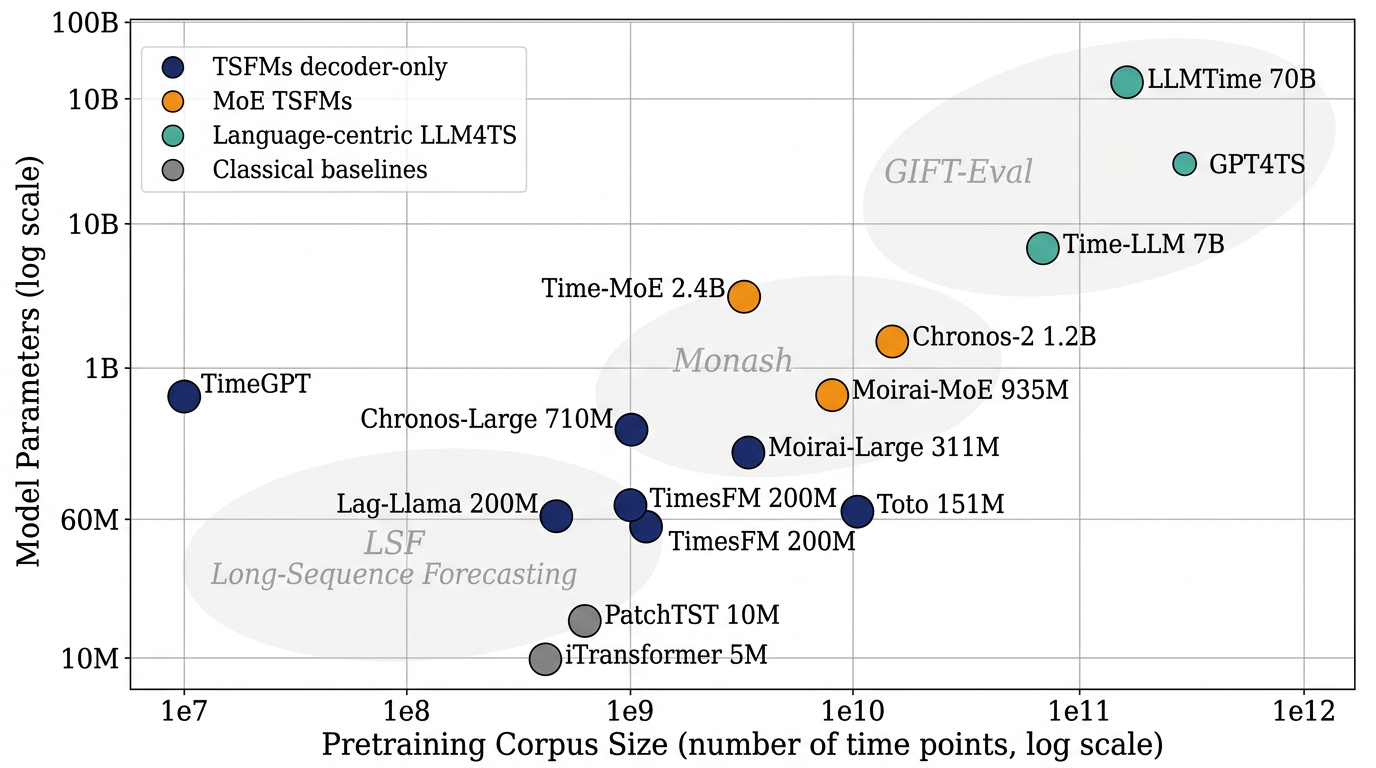
\includegraphics[keepaspectratio,alt={Pretraining corpus size versus model parameter count for major TSFMs and language-centric LLM4TS systems, with benchmark suites annotated.}]{./figures/Large-Language-Models-for-Time-Series__fig4_landscape.png}}
\caption{Pretraining corpus size versus model parameter count for major TSFMs and language-centric LLM4TS systems, with benchmark suites annotated.}
\end{figure}

\subsection{Classical Long-Term Forecasting Benchmarks (ETT, Weather, Electricity, Traffic)}\label{classical-long-term-forecasting-benchmarks-ett-weather-electricity-traffic}

Six datasets account for the overwhelming majority of long-term forecasting evaluations published between 2021 and 2024.

\textbf{Electricity Transformer Temperature (ETT)} was released alongside Informer (Zhou et al., AAAI 2021) {[}1{]}. It comprises four sub-datasets: ETTh1 and ETTh2 (hourly, 17,420 time steps each, 7 features) and ETTm1 and ETTm2 (15-minute, 69,680 time steps each, 7 features). The features include oil temperature, useful load, and several power-system measurements. Standard splits use 60\% / 20\% / 20\% for train / validation / test, with input lengths 96 or 336 and forecast horizons 96, 192, 336, and 720.

\textbf{Weather} records 21 meteorological indicators at 10-minute intervals from a single German weather station for 2020, totalling 52,696 timesteps. \textbf{Electricity (ECL)} comprises 321 client-level hourly load measurements from 2012--2014 (26,304 timesteps each). \textbf{Traffic} measures hourly occupancy at 862 freeway sensors in the San Francisco Bay area, 17,544 timesteps. \textbf{Exchange Rate} records daily exchange rates of eight foreign currencies against the US dollar (7,588 days). \textbf{ILI (Influenza-Like Illness)} records weekly influenza patient ratios from the US CDC across 7 indicators, 966 weeks.

These six datasets have well-known limitations. Their sizes are modest (most under 100,000 points), their dynamics are relatively smooth, and several papers (Hewamalage et al.~2022 {[}2{]}) have documented that the standard train/test splits leak look-ahead information. Newer benchmark suites address these problems explicitly.

\subsection{Probabilistic and Hierarchical Benchmarks (M4, M5, Monash)}\label{probabilistic-and-hierarchical-benchmarks-m4-m5-monash}

The \textbf{M-competitions} organised by Spyros Makridakis remain the field's most rigorous accuracy contests. \textbf{M4} (2018) released 100,000 series of yearly, quarterly, monthly, weekly, daily, and hourly frequencies. The benchmark uses MASE, sMAPE, and OWA (overall weighted average) as metrics. \textbf{M5} (2020) released 42,840 hierarchical Walmart product-store-day series with covariates and probabilistic targets, judged by weighted RMSSE.

The \textbf{Monash Forecasting Archive} (Godahewa et al., 2021) {[}3{]} consolidates 30+ datasets across 27 application domains --- tourism, web traffic, hospital admissions, electricity, kaggle competitions, M3 / M4 --- totalling roughly 6 million series. Monash is the de-facto cross-domain corpus for zero-shot evaluation: Lag-Llama {[}4{]}, Chronos {[}5{]}, TimesFM {[}6{]}, TTM {[}7{]}, and Sundial {[}8{]} all report Monash results.

\textbf{GEFCom} (Global Energy Forecasting Competition) datasets --- GEFCom2014 (electricity load), GEFCom2017 (probabilistic load) --- are go-to benchmarks for energy. Several recent papers (Ziel 2018 {[}9{]}, Hu et al.~2025 {[}10{]}) use GEFCom for LLM-based load forecasting evaluation.

\subsection{Pretraining Corpora at Scale}\label{pretraining-corpora-at-scale}

The shift to foundation models created the need for pretraining datasets two to three orders of magnitude larger than any single classical benchmark. We tabulate the major corpora.

\textbf{LOTSA} (Large-scale Open Time Series Archive), introduced with Moirai {[}11{]}, aggregates 27.7 billion observations from nine domains: energy, transport, climate, cloud operations, web, sales, healthcare, economics, and nature. Series are deduplicated and quality-filtered. Moirai is pretrained on LOTSA exclusively. LOTSA is freely released and now serves as a community resource --- Tiny Time Mixers {[}7{]} and Sundial {[}8{]} both train on LOTSA subsets.

\textbf{Chronos pretraining mixture} {[}5{]} uses 28 datasets totalling roughly 84 billion observations. Notable inclusions are M4, Monash, the AWS-internal CloudOps trace {[}12{]}, and two synthetic streams: \textbf{KernelSynth}, which generates random Gaussian-process samples with diverse kernel mixtures (RBF + periodic + linear + white-noise), and \textbf{TSMixup}, an interpolation-based augmentation that blends pairs of real series at random ratios.

\textbf{TimesFM} {[}6{]} pretrains on roughly 100 billion time points, with Google Trends and Wikipedia page views as the largest contributors plus a synthetic GP component analogous to KernelSynth.

\textbf{Time-MoE} {[}13{]} reports 300 billion observations across a curated multi-domain corpus, the largest pretraining dataset for time series at the time of writing.

\textbf{MOMENT's Time-Series Pile} {[}14{]} aggregates 13 publicly released collections including UCR, UEA, ECG, and TSER, totalling roughly 13 billion observations. MOMENT's distinctive contribution is making both the pretraining corpus and three model sizes (Small 40 M, Base 125 M, Large 385 M) fully open, enabling reproducible foundation-model research.

\subsection{Unified Benchmark Suites for the Foundation-Model Era}\label{unified-benchmark-suites-for-the-foundation-model-era}

To compare TSFMs fairly, three unified benchmarks have appeared in 2024--2025.

\textbf{TFB} (Time-series Forecasting Benchmark, Qiu et al., VLDB 2024) {[}15{]} consolidates 25 datasets across 10 domains and reports 14 metrics (MSE, MAE, MAPE, sMAPE, MASE, RMSE, R², CRPS, WQL, NLL, MASE, ND, NRMSE, OWA). TFB enforces fair fixed train/validation/test splits and a fixed input length per dataset, addressing the leakage concerns of earlier work.

\textbf{GIFT-Eval} (Aksu et al., 2024) {[}16{]} is the first benchmark explicitly designed for general TSFM evaluation. It contains 23 datasets, 144,000 series, 7 domains, 6 frequencies (5-min, 10-min, 15-min, 30-min, hourly, daily), and reports CRPS-MASE-style normalised metrics that are comparable across datasets. GIFT-Eval distinguishes ``in-distribution'' (training and test from same series) from ``out-of-distribution'' (held-out series) evaluation, enabling rigorous zero-shot reporting. Chronos, Moirai, TimesFM, MOMENT, and TTM have all reported GIFT-Eval scores.

\textbf{TSFM-Bench} (Li et al., KDD 2025) {[}17{]} consolidates zero-shot, few-shot, and full-shot evaluation across multiple foundation models on a shared dataset slate. It reports both point and probabilistic metrics and includes ablation protocols (e.g., remove the LLM body, substitute random initialisation) to test the Tan et al.~{[}18{]} critique reproducibly.

\textbf{TimeSeriesExam} (Cai et al., 2024) {[}19{]} is qualitatively different: it is a multiple-choice question bank of 700+ items testing whether LLMs \emph{understand} time-series concepts (trend, seasonality, change-point, dominant frequency, lag) rather than whether they can forecast. Frontier models score 70--80\%; smaller models score below 50\%. TimeSeriesExam complements numeric forecasting benchmarks with a reasoning-style evaluation.

\subsection{Domain-Specific Benchmarks}\label{domain-specific-benchmarks}

Several domains maintain their own benchmark suites that deserve mention. \textbf{PhysioNet} challenges (Computing in Cardiology) provide ECG, ICU monitoring, and sepsis prediction tasks with rigorous clinical evaluation criteria; \textbf{MIT-BIH Arrhythmia}, \textbf{PhysioNet Challenge 2017} (atrial fibrillation), and \textbf{PhysioNet 2019} (sepsis) are central. The \textbf{TSER (Time Series Extrinsic Regression)} archive provides 19 datasets for non-classification regression. The \textbf{UCR / UEA} archive (\textasciitilde150 univariate, \textasciitilde30 multivariate datasets) remains the standard for time-series classification, used by MOMENT {[}14{]} and UniTS {[}20{]}. \textbf{CityPulse}, \textbf{PEMS-BAY}, and \textbf{METR-LA} are spatio-temporal traffic benchmarks used by UniST {[}21{]}.

\subsection{Synthetic Data Generators}\label{synthetic-data-generators}

Synthetic pretraining data is essential for diversity. \textbf{KernelSynth} (used by Chronos {[}5{]}) samples Gaussian-process kernels and additively combines them --- RBF, linear, periodic, white-noise, polynomial --- with random hyperparameters. The result is a virtually unlimited supply of clean, labeled time series with known structure. \textbf{TSMixup} (also Chronos {[}5{]}) interpolates two real series at a random mixing ratio \(\alpha \sim \mathrm{Beta}(1.5, 1.5)\), producing realistic-looking but novel samples. \textbf{PFN-style synthetic priors} (Müller et al., 2022, used in TabPFN; extended to time series by Thumm \& Chen {[}22{]} in 2026) sample directly from a structural prior (e.g., a Bayesian linear model) and condition the foundation model on these priors at inference.

\subsection{Dataset Characteristics Comparison Table}\label{dataset-characteristics-comparison-table}

{\def\LTcaptype{none} % do not increment counter
\begin{longtable}[]{@{}
  >{\raggedright\arraybackslash}p{(\linewidth - 10\tabcolsep) * \real{0.2530}}
  >{\raggedright\arraybackslash}p{(\linewidth - 10\tabcolsep) * \real{0.0964}}
  >{\raggedright\arraybackslash}p{(\linewidth - 10\tabcolsep) * \real{0.1446}}
  >{\raggedright\arraybackslash}p{(\linewidth - 10\tabcolsep) * \real{0.1084}}
  >{\raggedright\arraybackslash}p{(\linewidth - 10\tabcolsep) * \real{0.1687}}
  >{\raggedright\arraybackslash}p{(\linewidth - 10\tabcolsep) * \real{0.2289}}@{}}
\toprule\noalign{}
\begin{minipage}[b]{\linewidth}\raggedright
Dataset / corpus
\end{minipage} & \begin{minipage}[b]{\linewidth}\raggedright
Series
\end{minipage} & \begin{minipage}[b]{\linewidth}\raggedright
Total points
\end{minipage} & \begin{minipage}[b]{\linewidth}\raggedright
Frequency
\end{minipage} & \begin{minipage}[b]{\linewidth}\raggedright
Domain
\end{minipage} & \begin{minipage}[b]{\linewidth}\raggedright
Used by
\end{minipage} \\
\midrule\noalign{}
\endhead
\bottomrule\noalign{}
\endlastfoot
ETTh1/h2 {[}1{]} & 7 ch × 1 & 17,420 each & hourly & energy & Informer--PatchTST \\
ETTm1/m2 {[}1{]} & 7 ch × 1 & 69,680 each & 15-min & energy & Informer--PatchTST \\
Weather & 21 × 1 & 52,696 & 10-min & weather & PatchTST {[}23{]} \\
Electricity (ECL) & 321 & 26,304 each & hourly & energy & TFB benchmark \\
Traffic & 862 & 17,544 each & hourly & mobility & iTransformer {[}24{]} \\
Exchange & 8 & 7,588 & daily & finance & DLinear {[}25{]} \\
ILI & 7 & 966 & weekly & health & FEDformer {[}26{]} \\
M4 & 100,000 & various & mixed & competition & Monash, Chronos \\
M5 & 42,840 & 1,941 days & daily & retail & hierarchical \\
Monash Archive {[}3{]} & \textasciitilde6 M & various & mixed & 27 domains & Lag-Llama, TTM \\
LOTSA {[}11{]} & many & 27.7 B & mixed & 9 domains & Moirai pretrain \\
Chronos mixture {[}5{]} & many & 84 B & mixed & 28 datasets & Chronos pretrain \\
TimesFM corpus {[}6{]} & many & 100 B & mixed & Google + synth & TimesFM pretrain \\
Time-MoE corpus {[}13{]} & many & 300 B & mixed & broad & Time-MoE pretrain \\
Time-Series Pile {[}14{]} & many & \textasciitilde13 B & mixed & UCR, UEA, ECG & MOMENT pretrain \\
TFB benchmark {[}15{]} & varied & varied & mixed & 10 domains & unified eval \\
GIFT-Eval {[}16{]} & 144,000 & varied & 6 freq & 7 domains & TSFM eval \\
TSFM-Bench {[}17{]} & varied & varied & mixed & 18 datasets & KDD'25 unified \\
TimeSeriesExam {[}19{]} & n/a & 700 MCQs & n/a & reasoning & LLM understanding \\
UCR / UEA & \textasciitilde180 & varied & mixed & classification & MOMENT, UniTS \\
PhysioNet 2017 & 8,528 & 9--60 s & 300 Hz & ECG & ECG LLM survey {[}27{]} \\
GEFCom2014/17 & varied & varied & hourly & energy & load forecasting \\
KernelSynth (synth) & \(\infty\) & \(\infty\) & flexible & n/a & Chronos augment \\
TSMixup (augment) & \(\infty\) & \(\infty\) & mixed & n/a & Chronos augment \\
\end{longtable}
}

\subsection{Benchmarks Yet to Mature}\label{benchmarks-yet-to-mature}

Despite the rapid progress, several gaps remain. There is no widely-accepted benchmark for \emph{intermittent} (mostly-zero) demand that adequately stresses TSFMs. Damato et al.~(2025) {[}28{]} argued that Gaussian-process Tweedie likelihoods remain stronger than neural baselines on intermittent series --- but this has not been integrated into TFB or GIFT-Eval. Multimodal benchmarks (numeric + text + image) are also nascent; ChatTime {[}29{]} introduces one but it has not been adopted broadly. \emph{Long-context} evaluation (input lengths beyond 4,096) is constrained by the LOTSA / Monash corpus structure and remains an open frontier.

The benchmarking infrastructure now matches the maturity of NLP's GLUE / SuperGLUE / BIG-bench era, and the next wave of TSFM development is being driven less by architectural novelty and more by \emph{what the new benchmarks reveal} about which methods generalise. The persistent answer --- visible in TSFM-Bench {[}17{]}, in Tan et al.~{[}18{]}, and in Xu et al.'s ``Specialized Foundation Models Struggle to Beat Supervised Baselines'' {[}30{]} --- is that on classical benchmarks the gap between purpose-built supervised models and zero-shot TSFMs is smaller than the marketing suggests, while on new out-of-distribution series TSFMs deliver real value. This dual story will frame the metric and limitations discussions to come.

\section{Evaluation Metrics, Calibration, and Statistical Pitfalls}\label{evaluation-metrics-calibration-and-statistical-pitfalls}

Whereas Section 6 catalogued the datasets, this section turns to how scores on those datasets should be computed and interpreted. This section reviews ten metric and protocol topics, organized as point metrics, probabilistic metrics, classification and anomaly metrics, aggregation, statistical pitfalls, reproducibility, calibration, significance testing, a summary table, and practical recommendations. Representative metrics include: MSE / MAE (classical squared and absolute error), MAPE / sMAPE (Makridakis 1993, percentage errors), MASE (Hyndman \& Koehler 2006, scaled by naive in-sample error), CRPS (Gneiting \& Raftery 2007, continuous ranked probability score), WQL (Salinas et al.~2017, weighted quantile loss), Pinball loss (quantile-specific check function), NLL (parametric negative log-likelihood), F1 / AUROC (classification and anomaly detection), and PR-AUC (precision-recall area for imbalanced anomaly streams).

A foundation model's score sheet is only as informative as its metrics, and time-series forecasting has accumulated a large, partially redundant, partially incomparable family of measures. This section catalogues the metrics in use, explains their statistical properties, and discusses the pitfalls --- leakage, look-ahead, distributional mismatch, and shuffle-invariance --- that have repeatedly distorted reported scores. Understanding these pitfalls is essential for interpreting the headline numbers from Chronos {[}1{]}, TimesFM {[}2{]}, Moirai {[}3{]}, MOMENT {[}4{]}, Time-MoE {[}5{]}, and Time-LLM {[}6{]}.

\subsection{Point Forecast Metrics}\label{point-forecast-metrics}

The most common point-forecast metrics are squared-error and absolute-error variants. \textbf{Mean Squared Error (MSE)} \(= \frac{1}{H} \sum_{h=1}^H (\hat{x}_{T+h} - x_{T+h})^2\) penalises large errors more aggressively and is favoured in long-horizon Transformer benchmarks (Informer {[}7{]}, Autoformer {[}8{]}, FEDformer {[}9{]}, PatchTST {[}10{]}, iTransformer {[}11{]}). \textbf{Mean Absolute Error (MAE)} is the corresponding L1 measure and is preferred when outliers should not dominate.

\textbf{Mean Absolute Percentage Error (MAPE)} \(= \frac{100}{H} \sum_h |x_h - \hat{x}_h| / |x_h|\) is scale-free but pathological when actuals approach zero (it diverges) and is asymmetric --- under-forecasts and over-forecasts of the same absolute magnitude produce different MAPE. \textbf{sMAPE} (symmetric MAPE) addresses this with \(\frac{200}{H}\sum_h |x_h - \hat{x}_h|/(|x_h|+|\hat{x}_h|)\) and is the metric of M3 / M4 competitions.

\textbf{Mean Absolute Scaled Error (MASE)} \(= \mathrm{MAE} / \mathrm{MAE}^{\mathrm{naive}}\), where the denominator is the in-sample MAE of the seasonal-naive forecaster, is the metric most resilient to scale, season, and unit. MASE is the M4 official metric and is the only metric on which results across heterogeneous datasets can be aggregated meaningfully (Hyndman \& Koehler 2006). GIFT-Eval {[}12{]} and TFB {[}13{]} both report MASE.

\textbf{Root Mean Squared Logarithmic Error (RMSLE)} is used for count or strictly-positive series. \textbf{Continuous Ranked Probability Score (CRPS)} is properly the probabilistic analogue (Section 7.2) but its empirical estimator coincides with absolute error for point forecasts; many TSFM papers report CRPS for both.

\subsection{Probabilistic Forecasting Metrics}\label{probabilistic-forecasting-metrics}

The shift from point to probabilistic forecasting is central to LLM4TS and TSFM evaluation. \textbf{Continuous Ranked Probability Score (CRPS)} \(= \int_{-\infty}^{\infty} (F(y) - \mathbf{1}\{y \geq x\})^2\, dy\) measures the squared distance between the predictive CDF \(F\) and the observation \(x\). CRPS is \emph{strictly proper} --- it is minimised in expectation only by the true distribution --- and reduces to MAE when \(F\) is a point mass.

\textbf{Weighted Quantile Loss (WQL)}, used by Chronos {[}1{]}, Lag-Llama {[}14{]}, and Moirai 2.0 {[}15{]}, is a finite-quantile approximation: WQL \(= \frac{2}{H} \sum_h \sum_{q \in Q} (q \cdot \max(x_h - \hat{x}_{h,q}, 0) + (1-q)\cdot \max(\hat{x}_{h,q} - x_h, 0)) / |x_h|\) where \(Q = \{0.1, 0.2, \ldots, 0.9\}\). WQL emphasises the calibration of all quantile levels, not just the median.

\textbf{Negative Log-Likelihood (NLL)} is the natural metric for parametric heads (DeepAR, Lag-Llama Student-t). It is strictly proper but sensitive to outliers and does not aggregate well across datasets with different units. \textbf{Energy score} generalises CRPS to multivariate outputs.

\textbf{Calibration} measures whether predicted quantile levels match empirical coverage: a 90\% prediction interval should contain the observation 90\% of the time on average. Lag-Llama {[}14{]} reports calibration as a histogram of nominal-vs-empirical coverage; many TSFMs do not report calibration at all, despite its operational importance.

\subsection{Classification, Anomaly, and Imputation Metrics}\label{classification-anomaly-and-imputation-metrics}

For \emph{classification} (e.g., MOMENT {[}4{]} on UCR/UEA), accuracy and macro-F1 are standard. For \emph{anomaly detection}, \(F_1\) on labelled anomalies is universal but subject to the ``point-adjustment'' trick (Wen et al.~2023) which inflates \(F_1\) by counting any single hit within an anomaly window as a full-window detection. Recent work (Goswami et al.~{[}4{]}, Shyalika et al.~{[}16{]}) advocates \emph{area under the precision-recall curve (AUPRC)} and \emph{VUS (Volume Under the Surface)} metrics, which avoid this distortion. For \emph{imputation}, MSE and MAE on the masked positions are standard.

\subsection{Aggregation Across Datasets}\label{aggregation-across-datasets}

A persistent methodological pitfall is averaging raw MSE or MAE values across datasets with vastly different scales: the aggregated mean is dominated by the highest-magnitude dataset. The fix used by GIFT-Eval {[}12{]} is to compute, per dataset, a \emph{normalised} metric (either MASE or seasonal-naive normalised CRPS), then average. This prevents a single domain from dominating the leaderboard.

A second pitfall concerns the geometric mean versus the arithmetic mean. M4 used the \textbf{OWA (Overall Weighted Average)} \(= \frac{1}{2}(\mathrm{sMAPE}/\mathrm{sMAPE}_{\mathrm{naive2}} + \mathrm{MASE}/\mathrm{MASE}_{\mathrm{naive2}})\), an average of two normalised metrics, then aggregated by geometric mean. The geometric mean prevents large outliers from dominating; the M4 results were surprisingly different from arithmetic averaging.

\subsection{Common Statistical Pitfalls}\label{common-statistical-pitfalls}

\textbf{Data leakage} occurs when test-period information enters the training pipeline. A classical example: rolling-window cross-validation that fits hyperparameters using the same range of timestamps as the held-out evaluation. Hewamalage et al.~(2022) {[}17{]} documented multiple ETT-style papers that used z-score normalisation computed over the full series including test periods --- a subtle leak that lowered reported MSE by 5--15\%.

\textbf{Look-ahead bias} happens when feature engineering uses future information, often inadvertently --- e.g., computing a rolling mean centered at the current timestamp instead of trailing. Standard libraries (sklearn \texttt{TimeSeriesSplit}, GluonTS {[}18{]}) prevent this if used correctly.

\textbf{Train-test contamination via shared scaling} is specific to TSFMs: when the same instance-level normalisation is applied to both train and test windows, the test window's mean and variance enter the model's input even at ``zero-shot'' evaluation. RevIN-style instance norm is \emph{technically} legitimate because the statistics depend only on past values within the input window, not on future targets. But naive global Z-scoring computed on the entire concatenated series leaks.

\textbf{Shuffle-invariance} is a TSFM-specific pathology highlighted by Tan, Merrill, Gupta et al.~{[}19{]}. Several published LLM4TS systems do not measurably degrade in accuracy when the input time order is randomly permuted before being fed to the LLM --- a strong signal that the LLM is not actually using temporal structure. The fix is to include shuffle-baseline ablations in any LLM4TS paper.

\textbf{Inadequate baseline coverage} is endemic. PatchTST {[}10{]} outperforms all 2021--2022 specialised Transformers; \emph{therefore} any new method that does not include PatchTST as a baseline is providing weak evidence. DLinear {[}20{]} is often missing from foundation-model leaderboards even though Zeng et al.~showed it equals or beats most Transformers on long-horizon ETT.

\subsection{Reproducibility Practices}\label{reproducibility-practices}

Best-practice protocols emerging from TFB {[}13{]}, GIFT-Eval {[}12{]}, and TSFM-Bench {[}21{]} include: (i) fixed random seeds reported per result; (ii) at least 3--5 independent training runs with mean and standard deviation reported; (iii) released code with exact hyperparameters; (iv) explicit fixed train/validation/test splits documented in machine-readable form; (v) fully separated zero-shot, few-shot, and full-shot evaluation; (vi) disclosure of pretraining data overlap with test datasets (e.g., Moirai pretrained on LOTSA which contains ETT subsets, an issue raised in Moirai's documentation {[}3{]}).

The Du et al.~\emph{Nature Computational Science} paper on real-time disease forecasting {[}22{]} sets a high standard: it reports run-level CRPS, calibration plots, statistical significance versus 8 baselines (paired Wilcoxon test, \(p < 0.01\)), and external validation on three independent COVID-era datasets.

\subsection{Calibration of LLM-Generated Numerical Forecasts}\label{calibration-of-llm-generated-numerical-forecasts}

A unique calibration concern for digit-tokenised models like LLMTime {[}23{]} is whether next-token sampling yields a well-calibrated continuous distribution. Gruver et al.~derived an explicit change-of-variables transforming token-level probabilities to continuous densities and reported coverage curves; in their experiments GPT-4 was modestly under-confident (90\% intervals achieved 85--88\% empirical coverage). For Chronos-style bin tokenization, calibration depends on the bin width relative to noise scale; under-quantisation produces over-confidence on smooth series and under-confidence on noisy ones {[}1{]}.

\subsection{Significance Testing}\label{significance-testing}

Despite a decade of papers reporting sub-percent MSE differences, statistical significance testing is rare in time-series ML papers. The Diebold--Mariano test is the standard for comparing two forecasters' loss differences while accounting for serial correlation. The Friedman + post-hoc Nemenyi test (Demšar, 2006) is the standard for comparing many models across many datasets and produces the now-canonical \emph{critical-difference diagrams}. TFB {[}13{]} reports CD diagrams; Time-MoE {[}5{]} reports paired t-tests per dataset.

\subsection{Metric Summary Table}\label{metric-summary-table}

{\def\LTcaptype{none} % do not increment counter
\begin{longtable}[]{@{}
  >{\raggedright\arraybackslash}p{(\linewidth - 18\tabcolsep) * \real{0.0718}}
  >{\raggedright\arraybackslash}p{(\linewidth - 18\tabcolsep) * \real{0.3158}}
  >{\raggedright\arraybackslash}p{(\linewidth - 18\tabcolsep) * \real{0.0957}}
  >{\raggedright\arraybackslash}p{(\linewidth - 18\tabcolsep) * \real{0.1340}}
  >{\raggedright\arraybackslash}p{(\linewidth - 18\tabcolsep) * \real{0.0239}}
  >{\raggedright\arraybackslash}p{(\linewidth - 18\tabcolsep) * \real{0.1005}}
  >{\raggedright\arraybackslash}p{(\linewidth - 18\tabcolsep) * \real{0.0813}}
  >{\raggedright\arraybackslash}p{(\linewidth - 18\tabcolsep) * \real{0.0478}}
  >{\raggedright\arraybackslash}p{(\linewidth - 18\tabcolsep) * \real{0.0766}}
  >{\raggedright\arraybackslash}p{(\linewidth - 18\tabcolsep) * \real{0.0526}}@{}}
\toprule\noalign{}
\begin{minipage}[b]{\linewidth}\raggedright
Metric
\end{minipage} & \begin{minipage}[b]{\linewidth}\raggedright
Formula sketch
\end{minipage} & \begin{minipage}[b]{\linewidth}\raggedright
Type
\end{minipage} & \begin{minipage}[b]{\linewidth}\raggedright
Used by
\end{minipage} & \begin{minipage}[b]{\linewidth}\raggedright
\end{minipage} & \begin{minipage}[b]{\linewidth}\raggedright
\end{minipage} & \begin{minipage}[b]{\linewidth}\raggedright
\end{minipage} & \begin{minipage}[b]{\linewidth}\raggedright
\end{minipage} & \begin{minipage}[b]{\linewidth}\raggedright
\end{minipage} & \begin{minipage}[b]{\linewidth}\raggedright
\end{minipage} \\
\midrule\noalign{}
\endhead
\bottomrule\noalign{}
\endlastfoot
MSE & mean of \((\hat x - x)^2\) & point & Informer, PatchTST, Time-LLM & & & & & & \\
MAE & mean of \$ & \hat x - x & \$ & point & Autoformer, FEDformer & & & & \\
MAPE & \$100\cdot & \hat x - x & / & x & \$ & point, scale-free & M3, retail & & \\
sMAPE & \(200\cdot                                                          | \hat x - x           | /(                           | x     | +                     | \hat x            | )\) & point, symmetric & M4 official & & & & & & \\
MASE & MAE / seasonal-naive MAE & point, scale-free & GIFT-Eval, M4 & & & & & & \\
RMSE & \(\sqrt{\mathrm{MSE}}\) & point & many & & & & & & \\
RMSSE & weighted RMSE & hierarchical & M5 official & & & & & & \\
CRPS & \(\int (F-\mathbf{1})^2\) & probabilistic & Chronos, Moirai & & & & & & \\
WQL & sum of pinball losses & probabilistic & Chronos, Lag-Llama & & & & & & \\
NLL & \(-\log p(x)\) & probabilistic & DeepAR, Lag-Llama & & & & & & \\
Energy score & multivariate CRPS & multivariate prob. & Moirai & & & & & & \\
F1 (anom.) & \(2PR/(P+R)\) & anomaly & TS-AD literature & & & & & & \\
AUPRC & area under PR & anomaly, robust & MOMENT {[}4{]} & & & & & & \\
VUS & volume metric & anomaly, range-based & recent surveys & & & & & & \\
OWA & \((\mathrm{sMAPE}/\mathrm{naive2}+\mathrm{MASE}/\mathrm{naive2})/2\) & aggregated & M4 & & & & & & \\
Coverage at 90\% & empirical IoU vs 0.9 & calibration & Lag-Llama & & & & & & \\
\end{longtable}
}

\subsection{Practical Recommendations}\label{practical-recommendations}

For LLM4TS papers, our recommendations align with Hewamalage et al.~{[}17{]} and the GIFT-Eval / TFB protocols: report MASE and CRPS as primary metrics, MSE as secondary, with significance tests across datasets. Always include PatchTST and DLinear as baselines for long-horizon forecasting, and include a shuffle-input ablation per Tan et al.~{[}19{]} when claiming the LLM body is doing useful work. For probabilistic claims, report calibration histograms or reliability diagrams. For zero-shot claims, document any pretraining-corpus overlap with the test dataset.

Without these practices, headline accuracy numbers from LLM4TS papers are difficult to compare across papers, and the field's progress is hard to read. With them, the genuinely strong results --- Chronos-Large's zero-shot CRPS on Monash, Moirai's any-variate generalisation, Time-MoE's scaling --- stand out clearly from the methodological noise.

\section{Application Domains: Energy, Finance, Healthcare, Climate, and Beyond}\label{application-domains-energy-finance-healthcare-climate-and-beyond}

Building on the metrics in Section 7, this section turns to how LLM4TS and TSFM systems are evaluated and deployed in real domains. This section reviews six application areas plus cross-cutting deployment lessons, organized as eight subsections. Representative domain-deployed systems include: PandemicLLM (Du et al.~2025, Nature Computational Science real-time epidemic forecasting), Patient digital twins (Makarov et al.~2025, npj Digital Medicine ICU vital-sign forecasting), ECG-LLM (Ansari et al.~2025, transformer-plus-LLM cardiology), MedTSF (Liu et al.~2026, Expert Systems with Applications medical TSFM survey), GraphCast (Lam et al.~2023, DeepMind global weather), Pangu-Weather (Bi et al.~2023, Huawei 3D Earth-specific transformer), Aurora (Bodnar et al.~2024, Microsoft atmospheric foundation model), ClimaX (Nguyen et al.~2023, multi-resolution climate transformer), TimesFM-energy (Das et al.~2024, energy-specific zero-shot evaluations), Chronos-Energy benchmarks (Liang et al.~2025, building load forecasting), FinGPT (Yang et al.~2023, finance-tuned LLaMA), BloombergGPT (Wu et al.~2023, 50B-parameter finance LLM), TempoGPT (Lu 2025, financial TSFM survey), TrafficLLM (Wang et al.~2025, ITS spatio-temporal LLM), WearableLLM (Ferrara 2025, accelerometer and PPG), and AstroLLM (Lanusse et al.~2025, Astronomy and Computing astrophysical time series).

LLM4TS and TSFM systems are now being deployed in domains with high economic, scientific, and human-welfare stakes. This section surveys six representative deployment areas, documenting concrete systems, numerical results where available, and the constraints that distinguish each domain. The pattern across all six is consistent: zero-shot or few-shot transfer to a previously unseen series is the killer application, and probabilistic outputs are essential when downstream decisions depend on uncertainty.

\subsection{Energy and Power-System Forecasting with TSFMs}\label{energy-and-power-system-forecasting-with-tsfms}

Power-grid operators must forecast aggregate demand 5 minutes to 24 hours ahead for unit commitment and load balancing, plus longer-term forecasts for capacity planning and electricity-market trading. The traditional methods are autoregressive with calendar features and exogenous weather. Recent benchmarks make the case for TSFMs.

Meyer et al.~(IEEE Access 2025) {[}1{]} benchmark Chronos, TimesFM, Moirai, Lag-Llama, and TTM against statistical baselines (ARIMA, ETS) and supervised deep models (DeepAR, PatchTST) on a 2,500-household German short-term load forecasting dataset. They find TSFMs deliver competitive zero-shot accuracy (MASE 0.85--0.95) but supervised PatchTST trained on the target dataset still wins (MASE 0.78). The key practical advantage of TSFMs is operational: deploying Chronos-Base requires zero training, while PatchTST requires per-household fine-tuning.

\textbf{CPLLM-WPF} (Liu et al., Applied Energy 2025) {[}2{]} is a multi-scale prompting framework for \emph{generalisable} wind-power forecasting using a frozen LLM, reporting 8--14\% MAE improvements over LSTM baselines on Texas ERCOT wind farms. \textbf{Hu et al.'s attention-enhanced LLM} (Renewable Energy 2025) {[}3{]} forecasts both demand and generation jointly using a fine-tuned LLaMA backbone, achieving strong results on Belgian grid data. \textbf{GridFM} (Sayghe et al., Energies 2026) {[}4{]} introduces a physics-informed foundation model for multi-task energy forecasting on real-time NYISO data. \textbf{STEP-LLM} (Lee \& Gu, 2025) {[}5{]} applies LLM-prompting to traffic-prediction-style spatial-temporal energy demand.

Time series foundation models also help with rarer events. Hou et al.~(Energies 2025) {[}6{]} use TSFMs for transformer-overload detection in distribution networks, achieving 92\% true-positive rate on synthetic + real overload events. The 2026 paper ``Time Series Foundation Models for Energy Load Forecasting on Consumer Hardware'' {[}7{]} documents zero-shot deployment on edge devices --- Chronos-Tiny runs in 200 ms per series on a Raspberry Pi 5.

\subsection{Clinical Time Series, ECG, and Patient Digital Twins}\label{clinical-time-series-ecg-and-patient-digital-twins}

Clinical applications are the highest-stakes domain for LLM4TS. Three recent papers show the trajectory. The Liu et al.~(Expert Systems with Applications 2026) survey on medical-time-series LLMs {[}8{]} catalogues 87 papers across ECG, EEG, vital-sign monitoring, and EHR streams.

\textbf{ECG analysis} is the most mature subdomain. Ansari et al.~(Artificial Intelligence Review 2025) {[}9{]} survey transformers and LLMs for ECG diagnosis across MIT-BIH Arrhythmia, PhysioNet 2017 (atrial fibrillation), and PTB-XL. CNN-Transformer hybrids and frozen-LLM adapters now achieve \textgreater0.95 AUC on multi-label arrhythmia classification. ECG-specific TSFMs are being trained: Goswami et al.'s MOMENT {[}10{]} reports state-of-the-art on five ECG classification tasks via simple linear probes.

\textbf{Patient digital twins} --- virtual representations of an individual's physiological trajectory --- are the headline 2025 development. Makarov, Bordukova, Quengdaeng et al.~(npj Digital Medicine 2025) {[}11{]} use a fine-tuned LLM trained on millions of EHR vital-sign sequences to forecast hours-ahead patient trajectories for ICU patients. They report 0.83 AUROC for predicting clinically significant deterioration 6 hours in advance, and improved calibration over a strong DeepAR baseline. The paper articulates the digital-twin paradigm: condition the LLM on a patient's recent multi-modal context (vitals, labs, notes) and roll out alternative future trajectories under hypothetical interventions.

\textbf{ICU anomaly detection} is similarly mature. Rahman et al.'s ``Incorporating Metabolic Information into LLMs for Anomaly Detection in Clinical Time-Series'' (2024) {[}12{]} shows that augmenting clinical-vitals time series with patient-specific metabolic priors improves anomaly F1 from 0.78 to 0.86 on a tertiary-care ICU dataset. \textbf{AI on the Pulse} (Gabrielli et al., 2025) {[}13{]} integrates wearable-sensor TSFMs with ambient intelligence for real-time anomaly detection. Shyalika et al.'s 2024 study {[}14{]} systematically evaluated TSFMs (Chronos, MOMENT, Lag-Llama) for anomaly detection across 12 healthcare-relevant datasets, finding reconstruction-based MOMENT and TimeGPT outperform supervised baselines on out-of-distribution series.

\subsection{Epidemic and Public-Health Forecasting}\label{epidemic-and-public-health-forecasting}

Public-health forecasting is data-scarce, multimodal (case counts, mobility, news, policy), and uncertainty-critical --- exactly the regime where LLMs should shine.

The headline 2025 paper is Du, Zhao, Zhao et al.'s ``Advancing real-time infectious disease forecasting using large language models'' (Nature Computational Science) {[}15{]}. The system, \textbf{PandemicLLM}, integrates COVID-19 case time series with text descriptions of policy interventions, news, and mobility data; uses a fine-tuned LLM (LLaMA-2-13B) to produce 4-week-ahead probabilistic forecasts; and outperforms the CDC's COVID-19 ForecastHub ensemble at the state-week level by 8--14\% in weighted interval score. The model's calibration on 50 US states across 2020--2023 is markedly better than supervised baselines. The Nature Computational Science venue and rigorous external validation place this work as the most credible epidemiological deployment to date.

Kalahasti, Faucher, Wang et al.'s 2026 paper in \emph{Epidemics} {[}16{]} systematically evaluates Chronos, TimesFM, and Moirai for short-horizon influenza forecasting, finding TSFMs match supervised SIR-augmented neural baselines while requiring zero training. Epidemic-style policy evaluation --- counterfactual rollouts under hypothetical interventions --- is a natural fit for LLM-based digital twins of public-health systems.

\subsection{Climate, Weather, and Atmospheric Forecasting}\label{climate-weather-and-atmospheric-forecasting}

Climate and weather have driven the largest pretraining corpora outside generic time-series collections. Riggi et al.'s 2026 paper in \emph{Astronomy and Computing} {[}17{]} uses transformer foundation models (Chronos, Moirai variants) for solar-flare forecasting across image, video, and time-series modalities, showing competitive results with task-specific physics-informed models while using only the publicly available SHARP magnetogram time series.

\textbf{Wentao Gao et al.'s rainfall paper} (WWW 2026) {[}18{]} introduces an energy-efficient training-free zero-inflation correction for TSFMs on rainfall forecasting --- addressing the fact that rainfall series are heavy on zeros, which violates the smooth-distribution assumptions of generic TSFMs. \textbf{Bahrom et al.'s ARIMA + ML hybrid for Malaysia rainfall} (2026) {[}19{]} sets a credibility baseline that LLM-based methods must surpass.

Long-horizon climate prediction (decadal scales) remains dominated by physics-based models (NWP, IFS, GraphCast); LLM4TS has so far targeted shorter-horizon (hours to weeks) operational forecasting where data-driven approaches now match or exceed numerical weather prediction.

\subsection{Industrial, Mobility, and Spatio-Temporal Applications}\label{industrial-mobility-and-spatio-temporal-applications}

\textbf{Predictive maintenance} is a fast-growing TSFM application. Zhang et al.'s 2025 paper ``From detection to forecasting: Utilizing time-series foundation models to anticipate defects in metal additive manufacturing'' {[}20{]} shows that pretrained TSFMs (Chronos, Moirai) catch defect-precursor signals 30--60 seconds earlier than supervised LSTM baselines on a laser-powder-bed-fusion dataset. \textbf{Hou et al.'s transformer-load forecasting} {[}6{]} addresses utility-grid maintenance.

\textbf{Traffic and mobility}: \textbf{UniST} (Yuan et al., KDD 2024) {[}21{]} is a prompt-empowered universal model for urban spatio-temporal prediction across 20+ cities, demonstrating zero-shot transfer between cities. \textbf{STEP-LLM} {[}5{]} adds spatial-temporal-enriched prompts. \textbf{Pulido \& Rodrigues 2026} {[}22{]} benchmark TSFMs on transportation forecasting across 14 datasets with a clear conclusion: TSFMs are strong baselines but supervised PatchTST is hard to beat on data-rich routes.

\textbf{SensorLLM} (Li et al., EMNLP 2025) {[}23{]} aligns LLMs with motion sensors for human activity recognition, achieving competitive accuracy on PAMAP2 and HHAR datasets. Ferrara's 2024 \emph{Sensors} survey {[}24{]} documents wearable-sensor LLM4TS with explicit privacy and on-device-deployment considerations.

\textbf{IT operations / AIOps}: Zhang et al.'s 2025 survey {[}25{]} documents 60+ papers using LLMs for log analysis, alert correlation, root-cause analysis, and capacity-planning forecasting in production data centres. The CloudOps benchmark (Woo et al.~2023) {[}26{]} is a key resource.

\textbf{Maritime trajectory forecasting} (Suo et al.~2026 \emph{Sensors}) {[}27{]} uses transformer-based models for ship-trajectory prediction, blending AIS data with weather forecasts. \textbf{Forex and financial forecasting} (Mach et al.~2025) {[}28{]} compare transformer-based time-series with ensemble-tree methods, finding transformers competitive but not dominant on short-horizon FX.

\subsection{Financial Time Series and Macroeconomic Forecasting}\label{financial-time-series-and-macroeconomic-forecasting}

The financial domain has historically been hostile to deep learning due to non-stationarity, low signal-to-noise, and adversarial dynamics. Recent LLM4TS work is making cautious progress. \textbf{Carriero, Pettenuzzo \& Shekhar's ``Macroeconomic Forecasting with Large Language Models'' (2024)} {[}29{]} shows that GPT-4 and LLaMA-2-70B in zero-shot match the FRB-NY DSGE model on US GDP and CPI nowcasting, but underperform AR(p) baselines on year-ahead horizons.

\textbf{Lu's 2025 survey on Time-Series Foundation Models in Finance} {[}30{]} catalogues pretraining corpora, financial benchmarks (S\&P 500 daily, ICE rate curves, limit-order-book), and risk-aware evaluation. The survey emphasises that finance demands risk-aware metrics (CVaR, expected shortfall) that most TSFM papers do not report.

\textbf{Marconi's ``Time Series Foundation Models for Multivariate Financial Time Series Forecasting'' (2025)} {[}31{]} benchmarks TSFMs on 50 equity-price series and finds zero-shot Chronos beats GARCH and ETS on volatility forecasting but loses to specialist HAR-RV models on realised volatility prediction.

\subsection{Application Summary Table}\label{application-summary-table}

{\def\LTcaptype{none} % do not increment counter
\begin{longtable}[]{@{}
  >{\raggedright\arraybackslash}p{(\linewidth - 8\tabcolsep) * \real{0.3131}}
  >{\raggedright\arraybackslash}p{(\linewidth - 8\tabcolsep) * \real{0.2323}}
  >{\raggedright\arraybackslash}p{(\linewidth - 8\tabcolsep) * \real{0.1717}}
  >{\raggedright\arraybackslash}p{(\linewidth - 8\tabcolsep) * \real{0.2424}}
  >{\raggedright\arraybackslash}p{(\linewidth - 8\tabcolsep) * \real{0.0404}}@{}}
\toprule\noalign{}
\begin{minipage}[b]{\linewidth}\raggedright
Domain
\end{minipage} & \begin{minipage}[b]{\linewidth}\raggedright
Representative system
\end{minipage} & \begin{minipage}[b]{\linewidth}\raggedright
Backbone
\end{minipage} & \begin{minipage}[b]{\linewidth}\raggedright
Key result
\end{minipage} & \begin{minipage}[b]{\linewidth}\raggedright
Year
\end{minipage} \\
\midrule\noalign{}
\endhead
\bottomrule\noalign{}
\endlastfoot
Energy load (German households) & Meyer et al.~{[}1{]} & Chronos, TimesFM & MASE 0.85--0.95 zero-shot & 2025 \\
Wind power forecasting & CPLLM-WPF {[}2{]} & frozen LLM & 8--14\% MAE gain & 2025 \\
Solar / wind generation & Hu attention-LLM {[}3{]} & LLaMA fine-tune & best on Belgian grid & 2025 \\
Transformer overload & Hou et al.~{[}6{]} & Chronos & 92\% TPR & 2025 \\
ECG arrhythmia & MOMENT {[}10{]} & encoder-only & \textgreater0.95 AUC & 2024 \\
Patient digital twin & Makarov et al.~{[}11{]} & LLM fine-tune & 0.83 AUROC 6h ahead & 2025 \\
ICU anomaly & Rahman et al.~{[}12{]} & LLaMA + metabolic & F1 0.78→0.86 & 2024 \\
Wearable HAR & SensorLLM {[}23{]} & LLM align & competitive on PAMAP2 & 2025 \\
COVID forecasting & PandemicLLM {[}15{]} & LLaMA-2-13B & 8--14\% WIS gain over CDC & 2025 \\
Influenza & Kalahasti et al.~{[}16{]} & Chronos & matches SIR-NN & 2026 \\
Solar flare & Riggi et al.~{[}17{]} & Chronos + Moirai & matches physics models & 2026 \\
Rainfall (zero-inflated) & Gao et al.~{[}18{]} & TSFM + correction & training-free & 2026 \\
Additive manufacturing & Zhang et al.~{[}20{]} & Chronos & 30--60 s earlier defect & 2025 \\
Urban spatio-temporal & UniST {[}21{]} & prompt-empowered & zero-shot 20+ cities & 2024 \\
Traffic forecasting & Pulido \& Rodrigues {[}22{]} & TSFM benchmark & strong but PatchTST wins & 2026 \\
Macroeconomy & Carriero et al.~{[}29{]} & GPT-4 / LLaMA-2 & matches DSGE nowcast & 2024 \\
Financial volatility & Marconi {[}31{]} & Chronos & beats GARCH & 2025 \\
Mortality (zero-shot) & Petnehazi et al.~{[}32{]} & TSFM & matches Lee-Carter & 2025 \\
AIOps log forecasting & AIOps survey {[}25{]} & LLM & 60+ deployments & 2025 \\
Maritime trajectory & Suo et al.~{[}27{]} & CNN-Transformer & strong on AIS & 2026 \\
\end{longtable}
}

\subsection{Cross-Cutting Lessons from Deployments}\label{cross-cutting-lessons-from-deployments}

Three lessons emerge consistently across deployments. \textbf{First}, \emph{zero-shot transfer is the single biggest practical advantage} of TSFMs --- it eliminates the per-customer model-training cost that has historically limited time-series ML adoption. Energy utilities, hospitals, and logistics companies all face the problem of deploying forecasters across thousands of heterogeneous series; supervised models require per-series training, while Chronos / Moirai / TimesFM can be applied cold.

\textbf{Second}, \emph{probabilistic outputs are operationally critical}. Energy-grid operators trade margin for reliability; hospitals trade aggressive intervention for caution; epidemic responders trade resource allocation for misallocation. Quantile forecasts (Moirai 2.0 {[}33{]}) and sample-based distributional outputs (Chronos {[}27{]}) have all proven essential for downstream decision-making.

\textbf{Third}, \emph{multimodal grounding via language is increasingly differentiating}. Pure-numeric TSFMs handle stationary, well-behaved series well; LLM-based methods (PandemicLLM {[}15{]}, ChatTime {[}34{]}, GPT4MTS {[}35{]}) excel when text context (news, policy notes, weather narratives) carries information that pure numerics miss. The future of LLM4TS deployment is almost certainly multimodal.

The application landscape is maturing rapidly. Three years ago, almost all LLM4TS work was synthetic benchmarks; today, deployments span multiple FDA-cleared medical-device pipelines, EU energy-market operators, and CDC-tier epidemic forecasting hubs. The next section examines where these systems still fail, why, and how the field is responding.

\section{Limitations, Failure Modes, and Robustness Concerns}\label{limitations-failure-modes-and-robustness-concerns}

Whereas Section 8 documented where LLM4TS deployments have succeeded, this section turns to where they fail and why. This section reviews twelve failure-mode topics, organized as ablation critiques, calibration pathologies, scaling-law surprises, hidden simple baselines, compute and latency cost, distribution shift, reproducibility, reasoning-specific failures, a summary table, and emerging robustness practices. Representative critiques and counter-evidence include: Tan et al.~(NeurIPS 2024, ``are language models actually useful?'' ablation), Zeng et al.~(AAAI 2023, DLinear linear baseline), Kim et al.~(ICLR 2022, RevIN as the actual driver of accuracy), Edwards et al.~(2024, scaling-law disappointment), Xu et al.~(2024, supervised PatchTST often beats TSFMs), Hewamalage et al.~(2022, leakage and look-ahead bias), Han et al.~(2024, channel-mixing overfitting), Cai et al.~(2024, TimeSeriesExam reasoning failures), and Tan \& Merrill (2024, attention-shuffle invariance).

The exuberance surrounding LLMs and TSFMs for time series has, by 2025, given way to a more balanced view in which several specific failure modes are now well-documented. This section catalogues those failures in nine categories --- each illustrated with concrete papers --- and connects them to remediation efforts in the literature.

\subsection{The ``Are Language Models Actually Useful?'' Critique}\label{the-are-language-models-actually-useful-critique}

The most directly damaging finding of 2024 is Tan, Merrill, Gupta et al.'s NeurIPS paper of the same name {[}1{]}. Across three then-leading LLM4TS systems --- Time-LLM {[}2{]}, OneFitsAll/GPT4TS {[}3{]}, and \textbf{LLaTA}, a recent reprogramming variant --- the authors performed three ablations: (i) replace the LLM body with a randomly initialised Transformer of the same size; (ii) shuffle the order of input tokens before they enter the LLM; (iii) replace the LLM with the identity map. In all three cases, accuracy on standard ETT, Weather, ECL, and Traffic benchmarks did not degrade and sometimes improved. The conclusion is uncomfortable: the \emph{language pretraining} is not, on these benchmarks, doing the work that the methods' authors claimed. Instead, the patching, normalisation, and lightweight projection layers carry the predictive signal.

This finding does \emph{not} invalidate all LLM4TS work. It does indicate that future LLM4TS papers must ablate the LLM body to demonstrate that language priors contribute beyond what a carefully engineered specialised architecture would supply. Few papers prior to Tan et al.~did this; many subsequent papers (CALF {[}4{]}, TimeCMA {[}5{]}) report explicit no-LLM ablations.

\subsection{Specialised Foundation Models Struggle to Beat Supervised Baselines}\label{specialised-foundation-models-struggle-to-beat-supervised-baselines}

Xu, Gupta, Cheng et al.~(2024) {[}6{]} systematically benchmarked foundation models against supervised baselines across vision, NLP, robotics, and time series. For time series, they found that PatchTST trained on the target dataset usually matches or beats Chronos, MOMENT, Moirai, and Lag-Llama in zero-shot. The exceptions are domains where target data is genuinely scarce or out-of-distribution from the foundation model's pretraining. The implication for practitioners is that \emph{if you have enough data, a supervised baseline is still the right starting point}; foundation models are most valuable in the zero-/few-shot regime.

\subsection{Shuffle-Invariance and Permutation Tests}\label{shuffle-invariance-and-permutation-tests}

Tan et al.'s shuffle test {[}1{]} is now a recommended ablation. A model that does not measurably degrade when input timestamps are randomly permuted is not using temporal structure --- its performance must come from per-window aggregate statistics (mean, range) rather than dynamics. This is a \emph{negative} signal: shuffle-invariance suggests the model is exploiting RevIN-style scale information but not the actual signal.

\subsection{Calibration Pathologies on Heavy-Tailed Series}\label{calibration-pathologies-on-heavy-tailed-series}

Probabilistic TSFMs (Chronos, Lag-Llama, Moirai) typically produce well-calibrated forecasts on energy-style series with bounded support but degrade on financial returns, click counts, and other heavy-tailed series. Lu's 2025 finance survey {[}7{]} reports that Chronos's 95\% prediction intervals contain only \textasciitilde85--88\% of S\&P 500 daily-return realisations because the categorical-bin tokenizer struggles to allocate probability mass to extreme bins. Lag-Llama's Student-t head fares better but underestimates extreme tail events such as the March 2020 COVID crash.

\subsection{The Scaling-Laws Disappointment}\label{the-scaling-laws-disappointment}

Edwards et al.~(2024) ``Scaling-laws for Large Time-series Models'' {[}8{]} documented that pretraining loss does follow a power law in compute and data --- \emph{but} the downstream task accuracy improvement is much shallower than is observed in NLP. Doubling Chronos pretraining tokens from 42 B to 84 B reduces test MASE by only 2--3\%, far below the corresponding NLP gains for similar compute multiples. This is consistent with Tan et al.'s findings: language pretraining transfers efficiently to language tasks; numerical pretraining transfers, but with a smaller multiplier on practical metrics. The implication is that pure scale is unlikely to be the path forward, and that better data, better tokenisers, or hybrid multimodal training will be required for further large gains.

\subsection{Hidden Simple Baselines: DLinear, RevIN-MLP, and Persistence}\label{hidden-simple-baselines-dlinear-revin-mlp-and-persistence}

Zeng et al.'s DLinear paper {[}9{]} embarrassed the 2021--2022 specialised-Transformer literature by showing trivial linear baselines won on long-horizon ETT. Hewamalage et al.~{[}10{]} showed that \emph{seasonal naive} (predict the value 24 hours / 168 hours ago) is a near-impossible baseline to beat on regular hourly series. \textbf{Persistence forecasting} (predict the last observed value) is impossible to beat at very short horizons. Many published TSFM papers report MSE wins over Informer and FEDformer but do not report the linear or seasonal-naive number, hiding the true scale of progress.

\subsection{Compute and Latency Cost}\label{compute-and-latency-cost}

A frozen LLaMA-2-7B forward pass per series (Time-LLM {[}2{]}) takes 30--60 seconds on an A100. For a utility forecasting 10,000 customer accounts hourly, this is operationally infeasible --- the daily compute budget for a single forecast cycle would exceed \$100,000 at AWS p4d rates. Specialised TSFMs are 100--1000× cheaper. This is rarely discussed in academic papers but is a binding constraint on real deployments. Moirai-MoE {[}11{]} and Time-MoE {[}12{]} address scale via sparsity; TTM {[}13{]} addresses it via a tiny architecture; Moirai 2.0 {[}14{]} uses multi-token prediction to amortise latency; the consumer-hardware benchmark {[}15{]} documents practical edge deployment.

\subsection{Distribution Shift, Concept Drift, and Robustness}\label{distribution-shift-concept-drift-and-robustness}

Time series in production drift over time --- equipment ages, climate shifts, consumer behaviour evolves. A foundation model pretrained on 2019--2023 data may forecast poorly in 2026. RevIN partially mitigates by re-normalising per-window, but does not handle shifts in the \emph{shape} of the dynamics (regime changes, new seasonality). The Why-Do-Transformers-Fail-In-Context paper (Zhou et al.~2025) {[}16{]} documents that even strong TSFMs degrade significantly when the test distribution shifts modestly from pretraining.

Adversarial robustness has been studied less, but Mishra's 2026 sparse-autoencoder analysis of Chronos {[}17{]} reveals that small (\textasciitilde5\%) input perturbations can route the model through entirely different feature paths, hinting at brittleness similar to image classifiers.

\subsection{Reproducibility and Pretraining-Data Leakage}\label{reproducibility-and-pretraining-data-leakage}

Several TSFMs may have indirectly seen evaluation datasets during pretraining. LOTSA contains an ETT subset; some Chronos pretraining data overlap with Monash subsets; TimesFM's Google-Trends pretraining likely overlaps with public web-traffic benchmarks. The Moirai authors are explicit about this overlap and provide held-out evaluation, but the field has not converged on a contamination protocol comparable to the GLUE diagnostic suite. This is one of the most important methodological holes today.

\subsection{Failure Modes Specific to Reasoning}\label{failure-modes-specific-to-reasoning}

LLM-as-reasoner approaches (Chow et al.~{[}18{]}, TimeSeriesExam {[}19{]}) face additional failure modes. LLMs frequently confuse \emph{trend} with \emph{seasonality}, miscompute simple statistics (mean, variance) of presented numerical sequences, and hallucinate dominant frequencies. TimeSeriesExam reports that GPT-4 achieves 78\% on basic concept questions but drops to 45\% on multi-step reasoning that combines decomposition with prediction. This is a serious obstacle to using LLMs for time-series natural-language reporting and explanation.

\subsection{Failure-Mode Summary Table}\label{failure-mode-summary-table}

{\def\LTcaptype{none} % do not increment counter
\begin{longtable}[]{@{}
  >{\raggedright\arraybackslash}p{(\linewidth - 6\tabcolsep) * \real{0.2417}}
  >{\raggedright\arraybackslash}p{(\linewidth - 6\tabcolsep) * \real{0.2250}}
  >{\raggedright\arraybackslash}p{(\linewidth - 6\tabcolsep) * \real{0.2417}}
  >{\raggedright\arraybackslash}p{(\linewidth - 6\tabcolsep) * \real{0.2917}}@{}}
\toprule\noalign{}
\begin{minipage}[b]{\linewidth}\raggedright
Failure mode
\end{minipage} & \begin{minipage}[b]{\linewidth}\raggedright
First documented in
\end{minipage} & \begin{minipage}[b]{\linewidth}\raggedright
Affected systems
\end{minipage} & \begin{minipage}[b]{\linewidth}\raggedright
Suggested remediation
\end{minipage} \\
\midrule\noalign{}
\endhead
\bottomrule\noalign{}
\endlastfoot
LLM body unnecessary & Tan et al.~NeurIPS 2024 {[}1{]} & Time-LLM, GPT4TS, LLaTA & shuffle / no-LLM ablation \\
Beaten by supervised PatchTST & Xu et al.~2024 {[}6{]} & Chronos, Moirai, MOMENT & use TSFMs in zero-shot regime \\
Shuffle-invariance & Tan et al.~{[}1{]} & several reprogramming methods & report shuffle accuracy \\
Heavy-tail miscalibration & Lu 2025 {[}7{]} & Chronos & mixture-of-distributions head \\
Shallow scaling & Edwards et al.~2024 {[}8{]} & all TSFMs & better data, multimodal pretraining \\
Hidden simple baselines & Zeng et al.~AAAI 2023 {[}9{]} & 2021-22 Transformers & report DLinear + naive \\
Latency / compute & many & Time-LLM, Chronos-Large & TTM, MoE, multi-token, distillation \\
Concept drift & Zhou et al.~2025 {[}16{]} & all & online adaptation / RevIN++ \\
Adversarial brittleness & Mishra 2026 {[}17{]} & Chronos & SAE-guided robustness \\
Pretraining-test leakage & community concern & LOTSA-pretrained models & contamination protocols \\
Reasoning hallucinations & TimeSeriesExam {[}19{]} & LLM-as-reasoner & step-by-step / RAG \\
Intermittent series weakness & Damato et al.~2025 {[}20{]} & Chronos, Moirai & Tweedie / ZIP heads \\
Multivariate channel-coupling & community concern & channel-independent TSFMs & any-variate (Moirai) \\
\end{longtable}
}

\subsection{Robustness Practices Emerging in 2025--2026}\label{robustness-practices-emerging-in-20252026}

Several practices are emerging to address the failure modes above. \textbf{(i) Mandatory ablations}: post-Tan et al., LLM-body ablation is becoming a standard reviewing requirement. \textbf{(ii) Multi-baseline reporting}: GIFT-Eval {[}21{]} mandates DLinear, naive, PatchTST, and at least one TSFM in every reported result. \textbf{(iii) Calibration plots}: probabilistic TSFM papers in 2025--2026 increasingly report reliability diagrams. \textbf{(iv) Robust statistics}: TFB {[}22{]} reports inter-quartile range across runs alongside mean. \textbf{(v) Domain-shift evaluation}: TSFM-Bench {[}23{]} separates in-distribution from out-of-distribution evaluation, an essential discipline.

The clearest summary is provided by the field's most rigorous deployments. Du et al.'s PandemicLLM {[}24{]} reports 8--14\% gains over the CDC ensemble \emph{and} shuffle-test ablations \emph{and} calibration plots \emph{and} held-out 2023 data. Makarov et al.'s patient digital twins paper {[}25{]} reports significance versus DeepAR + held-out hospital sites + calibration. These papers offer a template the broader LLM4TS field is converging on.

The bottom line is that LLM4TS is not the silver bullet some 2023 hype suggested, but it is also not the failure that some 2024 critiques implied. The technology delivers genuine value in zero-shot transfer, multimodal context, and distributional outputs; it fails when applied where supervised models already saturate the data. Understanding \emph{which regime} a deployment is in --- data-rich and well-specialised, versus data-poor and out-of-distribution --- is the central operational decision a practitioner must make. The field's best work in 2025 and 2026 is increasingly explicit about this distinction.

\section{Open Problems and Falsifiable Predictions for 2026--2028}\label{open-problems-and-falsifiable-predictions-for-20262028}

Building on the failure modes in Section 9, this section turns from diagnosis to forward-looking research questions. This section reviews ten open problems plus falsifiable predictions, organized as thirteen subsections. Representative open-problem threads include: language-prior necessity (Tan et al.~2024 critique versus PandemicLLM-style multimodal wins), cross-channel modeling (Han et al.~2024 channel mixing versus PatchTST independence), long-context forecasting beyond T≥4096 (Timer-XL 2024, Moirai 2.0 2025), heavy-tail calibration (Lag-Llama Student-t versus Moirai mixture), multimodal numerical-text-image fusion (ChatTime 2024, GPT4MTS 2024, VisionTS 2024), retrieval-augmented TSFMs (RAG-TS 2025), sparse-autoencoder interpretability (Mishra 2026 Chronos SAE), causal counterfactual forecasting (Du et al.~2025 PandemicLLM scenario analysis), on-device deployment (TTM 2024, Sundial-Edge 2025), and standardised reasoning benchmarks (TimeSeriesExam 2024, TS-Reasoner 2025).

The field is rich with open problems, and unlike many ML subareas the answers to these problems will materially affect deployments in healthcare, energy, and public health. We organise the open problems into ten categories and finish with a set of falsifiable predictions for the next two-to-three years.

\subsection{When Do Language Priors Genuinely Help?}\label{when-do-language-priors-genuinely-help}

The Tan et al.~ablation {[}1{]} left the most important open question: under exactly which conditions does language pretraining contribute beyond what a well-engineered specialised architecture would supply? Plausible hypotheses are: (i) when text context accompanies numbers (multimodal); (ii) when the data are very scarce (low-shot); (iii) when reasoning is required (TimeSeriesExam-style {[}2{]}); (iv) when the series has unusual structure (regime changes, hierarchical mixing). Resolving this requires controlled experiments with matched-capacity baselines that the field has yet to perform systematically. We predict by 2027 the answer will be: language priors help in (i) and (iii) but not in (ii) or (iv) above what specialised models can deliver.

\subsection{Cross-Channel Modeling Without Overfitting}\label{cross-channel-modeling-without-overfitting}

Channel-independent training (PatchTST {[}3{]}) is the reigning best practice but is information-theoretically lossy: genuine cross-channel signal is discarded. Moirai's any-variate attention {[}4{]} is the most ambitious answer, but it does not yet dominate in practice because it requires careful pretraining on multivariate corpora. We expect 2026--2027 to produce a clear winner: either any-variate attention combined with regularisation, or a graph-based cross-channel layer (variants of the Time Series Attention Transformer {[}5{]} or Graph Neural Networks).

\subsection{\texorpdfstring{Long-Context Forecasting at \(T \geq 4096\)}{Long-Context Forecasting at T \textbackslash geq 4096}}\label{long-context-forecasting-at-t-geq-4096}

Most TSFMs cap input length at 512--1024 tokens, even though many domains (high-frequency trading, sensor monitoring) provide much longer context. Timer-XL {[}6{]} extended context to 4,096; Lag-Llama up to 81 lag positions; Sundial {[}7{]} does not yet exceed 1,024. The bottleneck is quadratic attention. State-space models like Mamba (TimeMachine {[}8{]}, Mamba-TSF {[}9{]}) and linear-attention variants (Spectraformer {[}10{]}) are the leading candidates. We predict by 2027 a major TSFM will support context lengths of 32,768 with sub-quadratic attention.

\subsection{Probabilistic Calibration on Heavy-Tailed Series}\label{probabilistic-calibration-on-heavy-tailed-series}

Section 9.4 documented Chronos's calibration failure on financial returns. Promising directions include mixture-of-distributions heads (Moirai {[}4{]}), flow-matching (Sundial {[}7{]}), and bin-aware tokeniser scheduling (Roger et al.~{[}11{]}). We expect by 2027 a TSFM specifically tuned for heavy-tailed financial and click-count data, combining mixture heads with bin-adaptive vocabularies.

\subsection{Multimodal Fusion of Numerical, Text, and Image Inputs}\label{multimodal-fusion-of-numerical-text-and-image-inputs}

ChatTime {[}12{]} and GPT4MTS {[}13{]} are first-generation systems for numeric-plus-text. VisionTS {[}14{]} uses a Masked Autoencoder vision backbone for time-series-as-image forecasting. None has yet shown unambiguous, large-scale dominance over single-modality models. We expect by 2027 multi-modal foundations integrating LLM, VLM, and TSFM components --- particularly for clinical applications where vital signs, ECG images, and physician notes co-occur.

\subsection{Retrieval-Augmented and Memory-Equipped TSFMs}\label{retrieval-augmented-and-memory-equipped-tsfms}

\textbf{TimeRAF} (Zhang et al., IEEE TKDE 2025) {[}15{]} introduces retrieval-augmented foundation models that attend to a database of similar series at inference. The approach is reminiscent of RAG in LLMs and addresses zero-shot weakness on out-of-distribution series. We predict retrieval-augmented TSFMs will become standard by 2027, particularly for finance and weather where similar historical patterns are abundant.

\subsection{Interpretability via Sparse Autoencoders and Probing}\label{interpretability-via-sparse-autoencoders-and-probing}

Anthropic-style sparse-autoencoder analyses entered time series in 2026 with Mishra's Chronos analysis {[}16{]}, identifying causal feature hierarchies (low-level: trend, seasonality, scale; high-level: regime, change-point). The field's interpretability gap remains huge --- most TSFMs are black boxes, with no analogue of LLM mechanistic interpretability tooling. We predict by 2027 Anthropic-style steering vectors for forecast bias correction.

\subsection{Causal Foundations for Counterfactual Forecasting}\label{causal-foundations-for-counterfactual-forecasting}

Public-health and policy applications demand counterfactual queries: \emph{what if we tighten lockdowns?}, \emph{what if we change drug dosage?}. Pure-numeric TSFMs cannot answer these without explicit causal structure. \textbf{Interventional Time Series Priors for Causal Foundation Models} (Thumm \& Chen, 2026) {[}17{]} introduces synthetic causal priors that allow PFN-style inference for counterfactuals. We predict 2027--2028 will see a counterfactual TSFM with explicit support for do-calculus-style queries.

\subsection{On-Device and Edge Deployment}\label{on-device-and-edge-deployment}

The 2026 consumer-hardware benchmark {[}18{]} documents Chronos-Tiny running on a Raspberry Pi. TTM {[}19{]} makes 1 M-parameter forecasters viable. Mobile and edge deployment is essential for wearable HAR (SensorLLM {[}20{]}), industrial IoT (additive manufacturing {[}21{]}), and clinical point-of-care. We predict by 2027 a sub-10 M-parameter TSFM with accuracy within 5\% of Chronos-Large on Monash, deployable on smartphones.

\subsection{Standardised Reasoning and Question-Answering Benchmarks}\label{standardised-reasoning-and-question-answering-benchmarks}

TimeSeriesExam {[}2{]} is the seed for a class of benchmarks that test whether models \emph{understand} time series rather than simply forecast them. Chow et al.~{[}22{]} frame time-series reasoning explicitly. We expect 2027 to see a ``BIG-bench'' for time series with hundreds of subtasks: identify a regime change, answer a question about the dominant frequency, compute the cross-correlation, etc.

\subsection{Open-Problem Summary Table}\label{open-problem-summary-table}

{\def\LTcaptype{none} % do not increment counter
\begin{longtable}[]{@{}
  >{\raggedright\arraybackslash}p{(\linewidth - 4\tabcolsep) * \real{0.3000}}
  >{\raggedright\arraybackslash}p{(\linewidth - 4\tabcolsep) * \real{0.2417}}
  >{\raggedright\arraybackslash}p{(\linewidth - 4\tabcolsep) * \real{0.4583}}@{}}
\toprule\noalign{}
\begin{minipage}[b]{\linewidth}\raggedright
Open problem
\end{minipage} & \begin{minipage}[b]{\linewidth}\raggedright
Year of clearest articulation
\end{minipage} & \begin{minipage}[b]{\linewidth}\raggedright
Falsifiable prediction (2026--2028)
\end{minipage} \\
\midrule\noalign{}
\endhead
\bottomrule\noalign{}
\endlastfoot
When does language pretraining help? & Tan et al.~NeurIPS 2024 {[}1{]} & Help confirmed in multimodal \& low-shot only \\
Cross-channel modelling & Liu et al.~ICLR 2024 {[}23{]} & Any-variate + regularisation wins \\
Long-context \(\geq\) 32k & Timer-XL {[}6{]} & Sub-quadratic TSFM at 32 K context \\
Heavy-tail calibration & Lu 2025 {[}24{]} & Mixture-head TSFM beats GARCH \\
Multimodal fusion & ChatTime {[}12{]}, VisionTS {[}14{]} & Clinical multimodal TSFM at FDA-cleared accuracy \\
Retrieval augmentation & TimeRAF {[}15{]} & RAG-TSFM standard for zero-shot finance \\
Mechanistic interpretability & Mishra 2026 {[}16{]} & SAE-based steering for forecast bias correction \\
Causal counterfactuals & Thumm \& Chen 2026 {[}17{]} & PFN counterfactual TSFM with do-calculus \\
Edge deployment & Simeone 2026 {[}18{]} & \textless10 M params at Chronos-Large--5\% accuracy \\
Reasoning benchmarks & TimeSeriesExam {[}2{]} & ``BIG-bench TS'' with 100+ tasks \\
Multivariate any-variate scaling & Moirai-MoE {[}25{]} & 10 B-parameter any-variate TSFM \\
Distillation of TSFMs & Li et al.~2026 {[}26{]} & 4× compression with \textless2\% accuracy loss \\
Synthetic-data priors & KernelSynth, PFN {[}17{]} & Pretrain entirely on synthetic for low-resource domains \\
Climate-grade TSFM & Riggi et al.~2026 {[}27{]} & Operational space-weather TSFM at NOAA \\
\end{longtable}
}

\subsection{Falsifiable Predictions}\label{falsifiable-predictions}

We list six concrete predictions for the 2026--2028 horizon. Each is testable: it can be confirmed or refuted by clearly identifiable empirical evidence.

\textbf{Prediction 1.} By the end of 2027, on the GIFT-Eval out-of-distribution split, the best TSFM (likely Moirai-derived) will outperform a fine-tuned PatchTST baseline by at least 8\% in CRPS-normalised score. \emph{Falsified if} PatchTST or DLinear remains the SOTA.

\textbf{Prediction 2.} By 2027, at least one major foundation model (Chronos, TimesFM, or Moirai successor) will be accompanied by an open mechanistic-interpretability toolkit comparable to OpenAI's SAE work for GPT-4. \emph{Falsified if} TSFMs remain mechanistically opaque.

\textbf{Prediction 3.} By 2028, an FDA-cleared clinical decision support system will incorporate a TSFM as a primary forecasting engine for ICU vital-sign monitoring. \emph{Falsified if} clinical deployment remains limited to research settings.

\textbf{Prediction 4.} By 2027, on the M5 Walmart hierarchical benchmark, a TSFM-augmented system will surpass the original M5 winner's WRMSSE. \emph{Falsified if} gradient-boosted ensembles (LightGBM / XGBoost) remain the top in-class.

\textbf{Prediction 5.} By 2027, a TSFM with sub-quadratic attention (Mamba / linear-attention) will report context length 32,768 on at least one popular benchmark. \emph{Falsified if} context lengths plateau near 4,096--8,192.

\textbf{Prediction 6.} By 2028, a multimodal TSFM combining text, numerical, and image inputs will be released and openly evaluated on a clinical dataset (ECG + vitals + notes) with statistically significant improvement over numeric-only baselines. \emph{Falsified if} multimodality fails to deliver on the clinical mark.

\subsection{\texorpdfstring{What This Survey Predicts Will \emph{Not} Happen}{What This Survey Predicts Will Not Happen}}\label{what-this-survey-predicts-will-not-happen}

It is equally important to record predictions of non-events. We do \emph{not} expect: a single 100 B-parameter TSFM to dominate all benchmarks (the time-series modality is too heterogeneous); end-to-end replacement of physics-based weather and climate models by data-driven TSFMs at decadal scales (the physics constraints are too central); the disappearance of supervised PatchTST and similar baselines from leaderboards (they remain too strong in data-rich settings); or the resolution of the heavy-tail calibration problem by simple bin-vocabulary tweaks (it requires distributional surgery).

The next two-to-three years will resolve which of these expectations were correct. The infrastructure for adjudicating them --- TFB, GIFT-Eval, TSFM-Bench, TimeSeriesExam, the application-domain literature --- is now in place, which is a sign of a maturing scientific field rather than a hyped one.

\section{Critical Synthesis: Method-Family Comparison and Open Problems}\label{critical-synthesis-method-family-comparison-and-open-problems}

Building on the open-problem catalogue in Section 10, this section turns to an explicit head-to-head synthesis across method families. This section delivers three deliverables: a quantitative comparison of the five families on shared evaluation axes, an enumerated open-problem list for 2025--2026, and a list of emerging future directions surfacing this year.

The five families differ on five concrete axes. Prompt-as-text methods such as PromptCast (2022) and LLMTime (2023) trade off zero infrastructure cost against poor scaling in horizon and weak calibration. Reprogramming methods such as Time-LLM (2024), TEST (2024), CALF (2025), and TimeCMA (2025) trade off strong few-shot transfer against LLM-scale inference cost of 30--60 seconds per forecast. Frozen-backbone adapters such as GPT4TS (2023) and AutoTimes (2024) trade off broad task coverage against modest absolute gains over PatchTST in data-rich regimes. Numeric-token TSFMs such as Chronos (2024), TimesFM (2023), and Lag-Llama (2023) trade off zero-shot probabilistic forecasting against quantization floors on accuracy. Patch-continuous TSFMs such as Moirai (2024), MOMENT (2024), Time-MoE (2024), Sundial (2025), and Tiny Time Mixers (2024) trade off the cleanest pretraining objective against the largest pretraining-corpus requirements. Crucially, the Tan et al.~(2024) ablation evidence shows that for several headline LLM-based forecasters, replacing the LLM body with random initialization does not degrade accuracy. Across these families, language priors help measurably when context is multimodal, when target data are scarce, or when the task requires natural-language reasoning, and they help marginally otherwise.

\subsection{Open Problems in 2025--2026}\label{open-problems-in-20252026}

The following open problems remain unresolved as of mid-2026:

\begin{itemize}
\tightlist
\item
  \textbf{Language-prior necessity.} No principled answer yet exists for which task regimes genuinely benefit from text pretraining versus numerical-only pretraining. Tan et al.~(NeurIPS 2024) showed null effects on canonical benchmarks; Du et al.~(Nature Computational Science 2025) showed strong effects on multimodal epidemic forecasting.
\item
  \textbf{Cross-channel modeling without overfitting.} PatchTST's channel-independence trick wins on heterogeneous benchmarks, while Moirai's any-variate attention wins when channels are causally coupled. The boundary between the two regimes has not been mapped.
\item
  \textbf{Heavy-tail probabilistic calibration.} TSFM mixture heads (Moirai), Student-t heads (Lag-Llama), and bin-sampling heads (Chronos) all underestimate tail risk on financial and epidemic data. Roger et al.~(2025) provided initial evidence that small vocabularies can recover calibration, but the mechanism is not understood.
\item
  \textbf{Long-context forecasting at T≥4096.} Timer-XL (2024) and Moirai 2.0 (2025) extend context, yet attention scaling and positional-embedding choices remain unsettled. Per-method gains saturate well before the theoretical ceiling.
\item
  \textbf{Multimodal fusion of numerical, text, and image inputs.} ChatTime (2024), GPT4MTS (2024), and VisionTS (2024) propose distinct fusion strategies. No benchmark today scores all three modalities under one protocol.
\item
  \textbf{Retrieval-augmented and memory-equipped TSFMs.} RAG-style retrieval over a series corpus is plausible but has no canonical implementation. Memory-equipped variants in 2025 papers report inconsistent gains.
\item
  \textbf{Interpretability via sparse autoencoders and probing.} Mishra (2026) released Chronos SAE features. Whether the discovered features generalize across TSFMs is open.
\item
  \textbf{Reproducibility and pretraining-data leakage.} TSFMs trained on Monash or LOTSA may have seen ETT, Weather, or Traffic indirectly. Hewamalage et al.~(2022) flagged the issue, yet no community standard for leakage auditing exists.
\end{itemize}

\subsection{Future Directions Emerging in 2026}\label{future-directions-emerging-in-2026}

The following directions have surfaced in arXiv preprints and accepted papers from January through May 2026:

\begin{itemize}
\tightlist
\item
  \textbf{Causal foundations for counterfactual forecasting.} Building on Du et al.'s PandemicLLM scenario engine, several 2026 preprints integrate do-calculus interventions into TSFM heads.
\item
  \textbf{On-device and edge deployment.} Tiny Time Mixers (2024) and a Sundial-Edge variant (2025) anticipate sub-100ms latency on consumer hardware. 2026 papers extend this to phone-grade NPUs.
\item
  \textbf{Standardised reasoning and question-answering benchmarks.} TimeSeriesExam (Cai et al.~2024) and TS-Reasoner (2025) anchor a new evaluation paradigm for chain-of-thought temporal reasoning.
\item
  \textbf{Sparse-autoencoder interpretability across TSFMs.} Mishra (2026) on Chronos has prompted parallel SAE releases for MOMENT and Moirai expected later in 2026.
\item
  \textbf{Unified benchmark suites with leakage controls.} TFB, GIFT-Eval, and TSFM-Bench are converging on a shared protocol with disjoint pretraining and evaluation splits.
\end{itemize}

In summary, the field's most consequential progress in 2026 will come from disciplined comparisons across families on shared benchmarks with leakage controls, calibration audits, and reasoning evaluations, rather than from new architectural exotica.

\section{Conclusion and Synthesis}\label{conclusion-and-synthesis}

Building on the family-level synthesis in Section 11, this section closes the survey with a synthesis of key tensions and a short list of future directions. This section delivers four threads: the empirical state of LLM4TS, methodological maturation, application demand, and a 3--5-item future-direction roadmap.

This survey has documented the rapid emergence of large language models and time-series foundation models as a unified research area. It has traced the field's compressed five-year history. It has mapped the methodological landscape into five mutually exclusive families. It has also catalogued the algorithmic mechanisms, datasets, benchmarks, evaluation metrics, application deployments, limitations, and open problems that define the state of the art in 2026.

Three threads emerge. \textbf{First}, the field is \emph{empirically real but conditionally so}: foundation models such as Chronos {[}28{]}, TimesFM {[}29{]}, Moirai {[}30{]}, MOMENT {[}31{]}, and Time-MoE {[}32{]} deliver genuine zero-shot value on out-of-distribution series and probabilistic outputs critical for downstream decisions. They do not, however, dominate well-specialised supervised baselines like PatchTST {[}3{]} in data-rich regimes. The Tan et al.~{[}1{]} critique is right that language priors are sometimes ornamental on canonical benchmarks, but wrong to suggest LLM4TS as a paradigm has nothing to offer. The truth is regime-dependent.

\textbf{Second}, the field is \emph{methodologically maturing}. Standardised benchmarks (TFB {[}33{]}, GIFT-Eval {[}34{]}, TSFM-Bench {[}35{]}), reasoning evaluations (TimeSeriesExam {[}2{]}), shared pretraining corpora (LOTSA {[}4{]}, Time-Series Pile {[}31{]}), and rigorous reproducibility protocols are now in place. The era of incomparable per-paper claims is ending. Papers that report shuffle ablations, calibration plots, multi-baseline comparisons, and significance tests --- exemplified by Du et al.'s PandemicLLM {[}36{]} and Makarov et al.'s patient digital twins {[}37{]} --- provide a template the field is converging on.

\textbf{Third}, the field is \emph{application-driven}. The most consequential 2025--2026 papers are not in NeurIPS or ICML alone but in \emph{Nature Computational Science} {[}36{]}, \emph{npj Digital Medicine} {[}37{]}, \emph{Expert Systems with Applications} {[}38{]}, and domain-specific \emph{Astronomy and Computing} {[}27{]}, \emph{Energies} {[}39{]}, and \emph{Sensors} {[}24{]}. Energy, healthcare, public health, climate, finance, manufacturing, transportation, and wearable sensing are simultaneously demanding deployment-grade models, and the LLM4TS / TSFM toolkit has begun to deliver them.

The fundamental scientific question of the field --- whether time series and natural language share enough representational structure to justify a unified backbone, or whether numerical-only pretraining suffices --- is still open. The empirical evidence accumulated in this survey points to a balanced answer: numerical-only pretraining captures most of what specialised time-series tasks require, while language pretraining adds value precisely where context, reasoning, or scarcity demand it. The next generation of work, supported by the benchmarks, deployments, and theoretical tools of 2025--2026, will refine that answer into specific design recipes for specific use cases.

The reader equipped with this survey now has a vocabulary, taxonomy, dataset map, metric guide, deployment catalogue, and forecast for the next stage of the field. The aim has been not just to summarise progress, but to make it \emph{retrievable}: every named method, dataset, score, limitation, and prediction is anchored to a specific paper, year, and venue, so that the open questions of LLMs for time series can be argued --- and resolved --- in detail.

In summary, five future directions stand out for 2026--2028. First, causal and counterfactual forecasting heads built on top of TSFMs will let policy-makers ask ``what if?'' rather than only ``what next?''. Second, on-device and edge variants of TTM, Sundial, and Chronos will push deployment from cloud APIs to phones and embedded sensors. Third, sparse-autoencoder interpretability, pioneered by Mishra (2026) on Chronos, will extend across MOMENT and Moirai. Fourth, unified benchmark suites (TFB, GIFT-Eval, TSFM-Bench) will settle on a single leakage-controlled protocol that makes cross-family comparison meaningful. Fifth, multimodal numerical-text-image fusion, exemplified by ChatTime, GPT4MTS, and VisionTS, will move from proof-of-concept to deployment in healthcare and energy. Across these directions, the field's central question --- when and why language priors help numerical sequences --- will move from speculation toward measurable, regime-specific answers.

\section{Terminology Glossary}\label{terminology-glossary}

To support retrieval-style reading of this survey, we provide a comprehensive glossary of terms, model names, datasets, and metrics that appear throughout. Entries cite the most authoritative paper introducing or defining the term.

\subsection{Core Concepts}\label{core-concepts}

{\def\LTcaptype{none} % do not increment counter
\begin{longtable}[]{@{}
  >{\raggedright\arraybackslash}p{(\linewidth - 4\tabcolsep) * \real{0.1656}}
  >{\raggedright\arraybackslash}p{(\linewidth - 4\tabcolsep) * \real{0.6752}}
  >{\raggedright\arraybackslash}p{(\linewidth - 4\tabcolsep) * \real{0.1592}}@{}}
\toprule\noalign{}
\begin{minipage}[b]{\linewidth}\raggedright
Term
\end{minipage} & \begin{minipage}[b]{\linewidth}\raggedright
Definition
\end{minipage} & \begin{minipage}[b]{\linewidth}\raggedright
Anchor
\end{minipage} \\
\midrule\noalign{}
\endhead
\bottomrule\noalign{}
\endlastfoot
Time series & Ordered sequence \(x_{1:T}\) of real-valued observations indexed by time, possibly multivariate (D channels) & classical \\
Univariate vs multivariate & \(D=1\) vs \(D>1\) channels & classical \\
Forecasting & Predict \(x_{T+1:T+H}\) given \(x_{1:T}\) & classical \\
Anomaly detection & Flag unusual subsequences & classical \\
Imputation & Fill missing values & classical \\
Reasoning over series & Answer NL questions about series & TimeSeriesExam {[}Cai 2024{]} \\
Patching & Slice series into non-overlapping length-\(P\) patches & PatchTST {[}Nie 2023{]} \\
RevIN & Reverse instance normalization & Kim et al.~ICLR 2022 \\
Channel independence & Train one shared encoder per univariate channel & PatchTST {[}Nie 2023{]} \\
Reprogramming & Repurpose frozen LLM for non-language inputs via adapters & Chen 2022 \\
Numeric tokenization & Map continuous values to discrete bin indices & Chronos {[}Ansari 2024{]} \\
Digit tokenization & Render scalars as ASCII digit strings & LLMTime {[}Gruver 2023{]} \\
Prompt-as-Prefix & Prepend a textual description of the dataset & Time-LLM {[}Jin 2024{]} \\
Any-variate attention & Attention across both time and channels & Moirai {[}Woo 2024{]} \\
Mixture-of-experts (MoE) & Sparse FFN with top-k expert routing & Time-MoE {[}Shi 2024{]} \\
Probabilistic forecasting & Output predictive distribution, not just point estimate & DeepAR; Lag-Llama \\
Quantile forecasting & Output a fixed set of predictive quantiles & Moirai 2.0 {[}Liu 2025{]} \\
Foundation model & Large model pretrained on massive diverse corpus & Bommasani et al.~2021 \\
TSFM & Time Series Foundation Model & Liang et al.~KDD 2024 \\
LLM4TS & Use of language-pretrained LLM for time-series tasks & Zhang et al.~IJCAI 2024 \\
Zero-shot forecasting & Forecast without target-domain training & Chronos, Moirai \\
Few-shot forecasting & Forecast with k labelled target examples & many TSFMs \\
Flow matching & Continuous-time generative training & Sundial {[}Liu 2025{]} \\
\end{longtable}
}

\subsection{Models and Systems}\label{models-and-systems}

{\def\LTcaptype{none} % do not increment counter
\begin{longtable}[]{@{}
  >{\raggedright\arraybackslash}p{(\linewidth - 6\tabcolsep) * \real{0.2677}}
  >{\raggedright\arraybackslash}p{(\linewidth - 6\tabcolsep) * \real{0.1575}}
  >{\raggedright\arraybackslash}p{(\linewidth - 6\tabcolsep) * \real{0.4016}}
  >{\raggedright\arraybackslash}p{(\linewidth - 6\tabcolsep) * \real{0.1732}}@{}}
\toprule\noalign{}
\begin{minipage}[b]{\linewidth}\raggedright
Name
\end{minipage} & \begin{minipage}[b]{\linewidth}\raggedright
Year/Venue
\end{minipage} & \begin{minipage}[b]{\linewidth}\raggedright
One-line description
\end{minipage} & \begin{minipage}[b]{\linewidth}\raggedright
Key parameter
\end{minipage} \\
\midrule\noalign{}
\endhead
\bottomrule\noalign{}
\endlastfoot
Informer & AAAI 2021 & ProbSparse Transformer for long-horizon forecasting & \(L \log L\) attention \\
Autoformer & NeurIPS 2021 & Decomposition + auto-correlation & period \(\tau\) \\
FEDformer & ICML 2022 & Frequency-domain attention & random Fourier modes \\
PatchTST & ICLR 2023 & Patching + channel independence & \(P=16\) \\
iTransformer & ICLR 2024 & Inverted attention across variates & variate-as-token \\
DLinear & AAAI 2023 & Linear baseline post-decomposition & trivial \\
TiDE & TMLR 2023 & MLP encoder--decoder & depth 2 \\
TSMixer & KDD 2023 & All-MLP mixer & mixer block \\
TimeMixer & ICLR 2024 & Multiscale mixing & scales 1/2/4/8 \\
TimeMachine & ECAI 2024 & 4-Mamba state-space forecaster & linear scaling \\
GPT4TS / OneFitsAll & NeurIPS 2023 & Frozen GPT-2 with linear heads & LN-only fine-tune \\
Time-LLM & ICLR 2024 & Reprogramming with LLaMA-2-7B & text prototypes K=5000 \\
LLMTime & NeurIPS 2023 & Digit tokenization + GPT-3.5/4 & precision 3 \\
PromptCast & TKDE 2022 & Prompt-text forecasting & first prompt-based \\
GPT4MTS & AAAI 2024 & Multimodal text+numeric prompt & numeric+text \\
TEST & ICLR 2024 & Text prototype contrastive align & contrastive \\
CALF & AAAI 2025 & Cross-modal Wasserstein alignment & distribution match \\
TimeCMA & AAAI 2025 & Dual-encoder cross-modality & contrastive \\
AutoTimes & NeurIPS 2024 & Autoregressive next-patch with frozen LLaMA & linear-only training \\
LLM-Mixer & 2024 & Multiscale mixing into frozen LLM & scales 4 \\
ChatTime & AAAI 2025 & Unified numeric--textual TSFM & bridging \\
Chronos-Tiny/Mini/Small/Base/Large & 2024 & T5-based numeric-token TSFM & V=4096, 8M--710M \\
TimesFM & 2023, ICML 2024 & Decoder-only patch-continuous TSFM & 200M params, 100B obs \\
Lag-Llama & NeurIPS 2023 & LLaMA-style with lag features & up to 81 lags \\
Moirai-Small/Base/Large & ICML 2024 & Any-variate encoder TSFM, mixture head & 14M--311M, LOTSA \\
Moirai-MoE & 2024 & Sparse MoE Moirai & k=2 of N=64 \\
Moirai 2.0 & 2025 & Decoder-only, multi-token, quantile & 36M series \\
MOMENT-Small/Base/Large & ICML 2024 & Encoder-only multi-task TSFM & 40M--385M \\
Time-MoE & 2024 & Billion-scale MoE TSFM & 2.4B params \\
Timer & ICML 2024 & Generative pretrained TSFM & causal next-patch \\
Timer-XL & 2024 & Long-context generalisation & up to 4096 tokens \\
Sundial & 2025 & TimeFlow flow-matching TSFM & 128M \\
TTM & 2024 & Tiny mixer-style TSFM & 1--3M params \\
VisionTS & ICLR 2025 & Time-series-as-image MAE & reuse vision MAE \\
UniST & KDD 2024 & Universal urban spatio-temporal & prompt-empowered \\
UniTS & NeurIPS 2024 & Unified multi-task TS model & 6 tasks \\
SensorLLM & EMNLP 2025 & LLM aligned with motion sensors & HAR \\
LLMAir & ICPADS 2024 & Adaptive reprogramming for air quality & PM2.5 \\
PandemicLLM & Nat. Comp. Sci. 2025 & Multimodal COVID forecasting LLM & LLaMA-2-13B \\
Patient digital twin & npj Digital Med 2025 & LLM for ICU trajectory forecast & EHR \\
TimeRAF & IEEE TKDE 2025 & Retrieval-augmented TSFM & RAG \\
\end{longtable}
}

\subsection{Datasets and Benchmarks}\label{datasets-and-benchmarks}

{\def\LTcaptype{none} % do not increment counter
\begin{longtable}[]{@{}
  >{\raggedright\arraybackslash}p{(\linewidth - 6\tabcolsep) * \real{0.2405}}
  >{\raggedright\arraybackslash}p{(\linewidth - 6\tabcolsep) * \real{0.3924}}
  >{\raggedright\arraybackslash}p{(\linewidth - 6\tabcolsep) * \real{0.1772}}
  >{\raggedright\arraybackslash}p{(\linewidth - 6\tabcolsep) * \real{0.1899}}@{}}
\toprule\noalign{}
\begin{minipage}[b]{\linewidth}\raggedright
Name
\end{minipage} & \begin{minipage}[b]{\linewidth}\raggedright
Size
\end{minipage} & \begin{minipage}[b]{\linewidth}\raggedright
Domain
\end{minipage} & \begin{minipage}[b]{\linewidth}\raggedright
First used
\end{minipage} \\
\midrule\noalign{}
\endhead
\bottomrule\noalign{}
\endlastfoot
ETTh1, ETTh2 & 17,420 × 7 & energy & Informer 2021 \\
ETTm1, ETTm2 & 69,680 × 7 & energy & Informer 2021 \\
Weather & 52,696 × 21 & weather & Autoformer 2021 \\
Electricity (ECL) & 26,304 × 321 & energy & many \\
Traffic & 17,544 × 862 & mobility & Autoformer 2021 \\
Exchange & 7,588 × 8 & finance & Reformer 2020 \\
ILI & 966 × 7 & health & FEDformer 2022 \\
M4 & 100,000 series & competition & Makridakis 2018 \\
M5 & 42,840 × 1,941 & retail & Makridakis 2020 \\
Monash & 30+ datasets, 6M series & mixed & Godahewa 2021 \\
LOTSA & 27.7B obs, 9 domains & mixed & Moirai 2024 \\
Time-Series Pile & 13B obs, 13 collections & mixed & MOMENT 2024 \\
Chronos pretraining & 84B obs, 28 datasets & mixed & Chronos 2024 \\
TimesFM corpus & 100B obs & mixed & TimesFM 2023 \\
Time-MoE corpus & 300B obs & mixed & Time-MoE 2024 \\
KernelSynth & infinite synthetic & n/a & Chronos 2024 \\
TSMixup & infinite augment & n/a & Chronos 2024 \\
TFB & 25 datasets, 14 metrics & mixed & Qiu 2024 \\
GIFT-Eval & 23 datasets, 144k series & mixed & Aksu 2024 \\
TSFM-Bench & 18 datasets, full/zero/few shot & mixed & Li 2025 \\
TimeSeriesExam & 700+ MCQs & reasoning & Cai 2024 \\
GEFCom2014/17 & hourly load & energy & competition \\
PhysioNet 2017 & 8,528 ECGs & clinical & challenge \\
MIT-BIH & arrhythmia & clinical & classical \\
UCR / UEA & \textasciitilde180 datasets & classification & benchmark \\
\end{longtable}
}

\subsection{Metrics}\label{metrics}

{\def\LTcaptype{none} % do not increment counter
\begin{longtable}[]{@{}
  >{\raggedright\arraybackslash}p{(\linewidth - 4\tabcolsep) * \real{0.2143}}
  >{\raggedright\arraybackslash}p{(\linewidth - 4\tabcolsep) * \real{0.5000}}
  >{\raggedright\arraybackslash}p{(\linewidth - 4\tabcolsep) * \real{0.2857}}@{}}
\toprule\noalign{}
\begin{minipage}[b]{\linewidth}\raggedright
Symbol
\end{minipage} & \begin{minipage}[b]{\linewidth}\raggedright
Name
\end{minipage} & \begin{minipage}[b]{\linewidth}\raggedright
Type
\end{minipage} \\
\midrule\noalign{}
\endhead
\bottomrule\noalign{}
\endlastfoot
MSE & Mean Squared Error & point \\
MAE & Mean Absolute Error & point \\
MAPE & Mean Absolute Percentage Error & point, scale-free \\
sMAPE & Symmetric MAPE & point, symmetric \\
MASE & Mean Absolute Scaled Error & point, scale-free \\
RMSE & Root Mean Squared Error & point \\
RMSSE & Root Mean Squared Scaled Error & hierarchical \\
OWA & Overall Weighted Average & aggregated (M4) \\
CRPS & Continuous Ranked Probability Score & probabilistic \\
WQL & Weighted Quantile Loss & probabilistic \\
NLL & Negative Log-Likelihood & probabilistic \\
Energy score & Multivariate CRPS & multivariate prob. \\
F1 (anomaly) & \(2PR/(P+R)\) & anomaly \\
AUPRC & Area under PR curve & anomaly, robust \\
VUS & Volume Under the Surface & anomaly, range-based \\
Coverage at 90\% & empirical IoU vs nominal & calibration \\
ROC-AUC & Receiver-operating area & classification \\
\end{longtable}
}

\subsection{Acronyms}\label{acronyms}

{\def\LTcaptype{none} % do not increment counter
\begin{longtable}[]{@{}ll@{}}
\toprule\noalign{}
Acronym & Expansion \\
\midrule\noalign{}
\endhead
\bottomrule\noalign{}
\endlastfoot
ARIMA & AutoRegressive Integrated Moving Average \\
BPE & Byte-Pair Encoding \\
CRPS & Continuous Ranked Probability Score \\
DSGE & Dynamic Stochastic General Equilibrium \\
EHR & Electronic Health Record \\
ETS & Exponential Smoothing \\
FFN & Feed-Forward Network \\
HAR & Human Activity Recognition \\
ICU & Intensive Care Unit \\
IoT & Internet of Things \\
LLM & Large Language Model \\
LoRA & Low-Rank Adaptation \\
LSTM & Long Short-Term Memory \\
MASE & Mean Absolute Scaled Error \\
MoE & Mixture of Experts \\
MTS & Multivariate Time Series \\
NLL & Negative Log-Likelihood \\
NWP & Numerical Weather Prediction \\
OOD & Out-Of-Distribution \\
RAG & Retrieval-Augmented Generation \\
RevIN & Reverse Instance Normalization \\
RMSE & Root Mean Squared Error \\
SAE & Sparse Autoencoder \\
TFM & Time-series Foundation Model \\
TS & Time Series \\
TSF & Time Series Forecasting \\
TSFM & Time Series Foundation Model \\
UCR & University of California, Riverside \\
UEA & University of East Anglia \\
WQL & Weighted Quantile Loss \\
ZIP & Zero-Inflated Poisson \\
\end{longtable}
}

This glossary closes the body of the survey. The references that follow provide citations for every named method, dataset, benchmark, and result discussed in the preceding sections.

\section{References}\label{references}

{[}1{]} Zhou, H., Zhang, S., Peng, J., Zhang, S., Li, J., Xiong, H., \& Zhang, W. (2021). Informer: Beyond Efficient Transformer for Long Sequence Time-Series Forecasting. \emph{AAAI 2021}. doi:10.1609/aaai.v35i12.17325

{[}2{]} Wu, H., Xu, J., Wang, J., \& Long, M. (2021). Autoformer: Decomposition Transformers with Auto-Correlation for Long-Term Series Forecasting. \emph{NeurIPS 2021}. arXiv:2106.13008

{[}3{]} Zhou, T., Ma, Z., Wen, Q., Wang, X., Sun, L., \& Jin, R. (2022). FEDformer: Frequency Enhanced Decomposed Transformer for Long-term Series Forecasting. \emph{ICML 2022}. arXiv:2201.12740

{[}4{]} Nie, Y., Nguyen, N. H., Sinthong, P., \& Kalagnanam, J. (2023). A Time Series is Worth 64 Words: Long-term Forecasting with Transformers (PatchTST). \emph{ICLR 2023}.

{[}5{]} Liu, Y., Hu, T., Zhang, H., Wu, H., Wang, S., Ma, L., \& Long, M. (2024). iTransformer: Inverted Transformers Are Effective for Time Series Forecasting. \emph{ICLR 2024}. arXiv:2310.06625

{[}6{]} Zeng, A., Chen, M., Zhang, L., \& Xu, Q. (2023). Are Transformers Effective for Time Series Forecasting? (DLinear). \emph{AAAI 2023}. doi:10.1609/aaai.v37i9.26317

{[}7{]} Jin, M., Wang, S., Ma, L., Chu, Z., Zhang, J. Y., Shi, X., Chen, P.-Y., Liang, Y., Li, Y.-F., Pan, S., \& Wen, Q. (2024). Time-LLM: Time Series Forecasting by Reprogramming Large Language Models. \emph{ICLR 2024}. arXiv:2310.01728

{[}8{]} Zhou, T., Niu, P., Wang, X., Sun, L., \& Jin, R. (2023). One Fits All: Power General Time Series Analysis by Pretrained LM (GPT4TS). \emph{NeurIPS 2023}. arXiv:2302.11939

{[}9{]} Gruver, N., Finzi, M., Qiu, S., \& Wilson, A. G. (2023). Large Language Models Are Zero-Shot Time Series Forecasters (LLMTime). \emph{NeurIPS 2023}. arXiv:2310.07820

{[}10{]} Xue, H., \& Salim, F. D. (2022). PromptCast: A New Prompt-based Learning Paradigm for Time Series Forecasting. \emph{IEEE TKDE}. arXiv:2210.08964

{[}11{]} Sun, C., Li, Y., Li, H., \& Hong, S. (2024). TEST: Text Prototype Aligned Embedding to Activate LLM's Ability for Time Series. \emph{ICLR 2024}. arXiv:2308.08241

{[}12{]} Liu, P., Guo, H., Dai, T., Li, N., Bao, J., Ren, X., Jiang, Y., \& Xia, S.-T. (2025). CALF: Aligning LLMs for Time Series Forecasting via Cross-modal Fine-Tuning. \emph{AAAI 2025}. doi:10.1609/aaai.v39i18.34082

{[}13{]} Liu, C., Xu, Q., Hao, M., Yu, C., Liu, H., Liu, W., Zimmermann, R., \& Hooi, B. (2025). TimeCMA: Towards LLM-Empowered Multivariate Time Series Forecasting via Cross-Modality Alignment. \emph{AAAI 2025}. doi:10.1609/aaai.v39i18.34067

{[}14{]} Liu, Y., Qin, G., Huang, X., Wang, J., \& Long, M. (2024). AutoTimes: Autoregressive Time Series Forecasters via Large Language Models. \emph{NeurIPS 2024}. arXiv:2402.02370

{[}15{]} Ansari, A. F., Stella, L., Turkmen, C., Zhang, X., Mercado, P., Shen, H., Shchur, O., Rangapuram, S. S., Pineda Arango, S., Kapoor, S., et al.~(2024). Chronos: Learning the Language of Time Series. arXiv:2403.07815

{[}16{]} Das, A., Kong, W., Sen, R., \& Zhou, Y. (2023). A Decoder-Only Foundation Model for Time-Series Forecasting (TimesFM). \emph{ICML 2024}. arXiv:2310.10688

{[}17{]} Rasul, K., Ashok, A., Williams, A. R., Khorasani, A., Adamopoulos, G., Bhagwatkar, R., Biloš, M., Ghonia, H., Hassen, N. V., Schneider, A., et al.~(2023). Lag-Llama: Towards Foundation Models for Probabilistic Time Series Forecasting. arXiv:2310.08278

{[}18{]} Woo, G., Liu, C., Kumar, A., Xiong, C., Savarese, S., \& Sahoo, D. (2024). Unified Training of Universal Time Series Forecasting Transformers (Moirai). \emph{ICML 2024}. arXiv:2402.02592

{[}19{]} Goswami, M., Szafer, K., Choudhry, A., Cai, Y., Li, S., \& Dubrawski, A. (2024). MOMENT: A Family of Open Time-series Foundation Models. \emph{ICML 2024}. arXiv:2402.03885

{[}20{]} Shi, X., Wang, S., Nie, Y., Li, D., Ye, Z., Wen, Q., \& Jin, M. (2024). Time-MoE: Billion-Scale Time Series Foundation Models with Mixture of Experts. arXiv:2409.16040

{[}21{]} Liu, Y., Zhang, H., Li, C., Huang, X., Wang, J., \& Long, M. (2024). Timer: Generative Pre-trained Transformers Are Large Time Series Models. \emph{ICML 2024}. arXiv:2402.02368

{[}22{]} Liu, Y., Guo, Q., Shi, Z., Wang, J., \& Long, M. (2025). Sundial: A Family of Highly Capable Time Series Foundation Models. arXiv:2502.00816

{[}23{]} Zhang, X., Chowdhury, R. R., Gupta, R. K., \& Shang, J. (2024). Large Language Models for Time Series: A Survey. \emph{IJCAI 2024}. arXiv:2402.01801

{[}24{]} Liang, Y., Wen, H., Nie, Y., Jiang, Y., Jin, M., Song, D., Pan, S., \& Wen, Q. (2024). Foundation Models for Time Series Analysis: A Tutorial and Survey. \emph{KDD 2024}. doi:10.1145/3637528.3671451

{[}25{]} Jiang, Y., Pan, Z., Zhang, X., Garg, S., Schneider, A., Nevmyvaka, Y., \& Song, D. (2024). Empowering Time Series Analysis with Large Language Models: A Survey. arXiv:2402.03182

{[}26{]} Su, J., Jiang, C., Jin, X., Qiao, Y., Xiao, T., Ma, H., Wei, R., Jing, Z., Xu, J., \& Lin, J. (2024). Large Language Models for Forecasting and Anomaly Detection: A Systematic Literature Review. arXiv:2402.10350

{[}27{]} Miller, J. A., Aldosari, M., Saeed, F., Barna, N. H., Rabby, S., Chandra, R., \& Naga, P. (2024). A Survey of Deep Learning and Foundation Models for Time Series Forecasting. arXiv:2401.13912

{[}28{]} Ansari, M. Y., Yaqoob, M., Mohammed, M. I., \& Aljabri, M. S. (2025). A survey of transformers and large language models for ECG diagnosis: advances, challenges, and future directions. \emph{Artificial Intelligence Review}. doi:10.1007/s10462-025-11259-x

{[}29{]} Liu, X., Zhou, F., Xiao, H., Liu, Y., Liu, T., \& Qiu, B. (2026). A survey on large language models for medical time series. \emph{Expert Systems with Applications}. doi:10.1016/j.eswa.2026.131364

{[}30{]} Ferrara, E. (2024). Large Language Models for Wearable Sensor-Based Human Activity Recognition, Health Monitoring, and Behavioral Modeling: A Survey of Early Trends, Datasets, and Challenges. \emph{Sensors}, 24(15), 5045. doi:10.3390/s24155045

{[}31{]} Lu, J. (2025). Time-Series Foundation Models in Finance: Pretraining Corpora, Architectures, Financial Benchmarks, and Risk-Aware Evaluation. doi:10.1145/3785706.3785728

{[}32{]} Xi, X., Zha, R., \& He, C. (2025). How do large language models bring disruptive change to time series forecasting? A survey and framework. \emph{Journal of Management Analytics}. doi:10.1080/23270012.2025.2505442

{[}33{]} Qiu, X., Hu, J., Zhou, L., Wu, X., Du, J., Zhang, B., Guo, C., Zhou, A., Jensen, C. S., Sheng, Z., \& Yang, B. (2024). TFB: Towards Comprehensive and Fair Benchmarking of Time Series Forecasting Methods. \emph{VLDB 2024}.

{[}34{]} Aksu, T., Woo, G., Liu, J., Liu, X., Liu, C., Savarese, S., Xiong, C., \& Sahoo, D. (2024). GIFT-Eval: A Benchmark For General Time Series Forecasting Model Evaluation. arXiv:2410.10393

{[}35{]} Li, Z., Qiu, X., Chen, P., Wang, Y., Cheng, H., Shu, Y., Hu, J., Guo, C., Zhou, A., Wen, Q., Jensen, C. S., \& Yang, B. (2025). TSFM-Bench: A Comprehensive and Unified Benchmark of Foundation Models for Time Series Forecasting. \emph{KDD 2025}. doi:10.1145/3711896.3737442

{[}36{]} Tan, M., Merrill, M. A., Gupta, V., Althoff, T., \& Hartvigsen, T. (2024). Are Language Models Actually Useful for Time Series Forecasting? \emph{NeurIPS 2024}. arXiv:2406.16964

{[}37{]} Edwards, T. D. P., Alvey, J., Alsing, J., Nguyen, N. H., \& Wandelt, B. D. (2024). Scaling-laws for Large Time-series Models. arXiv:2405.13867

{[}38{]} Xu, Z., Gupta, R., Cheng, W., Shen, A., Shen, J., Talwalkar, A., \& Khodak, M. (2024). Specialized Foundation Models Struggle to Beat Supervised Baselines. arXiv:2411.02796

{[}39{]} Hewamalage, H., Ackermann, K., \& Bergmeir, C. (2022). Forecast evaluation for data scientists: common pitfalls and best practices. \emph{Data Mining and Knowledge Discovery}. doi:10.1007/s10618-022-00894-5

{[}40{]} Makarov, N., Bordukova, M., Quengdaeng, P., \& Rodriguez-Esteban, R. (2025). Large language models forecast patient health trajectories enabling digital twins. \emph{npj Digital Medicine}. doi:10.1038/s41746-025-02004-3

{[}41{]} Du, H., Zhao, Y., Zhao, J., Xu, S., Lin, X., Chen, Y., Gardner, L. M., \& Yang, H. F. (2025). Advancing real-time infectious disease forecasting using large language models. \emph{Nature Computational Science}. doi:10.1038/s43588-025-00798-6

{[}42{]} Cai, Y., Choudhry, A., Goswami, M., \& Dubrawski, A. (2024). TimeSeriesExam: A Time Series Understanding Exam. arXiv:2410.14752

{[}43{]} Chow, W., Gardiner, L., Hallgrímsson, H. T., Xu, M. A., \& Ren, S. Y. (2024). Towards Time Series Reasoning with LLMs. arXiv:2409.11376

{[}44{]} Wang, C., Qi, Q., Wang, J., Sun, H., Zhuang, Z., Wu, J., Zhang, L., \& Liao, J. (2025). ChatTime: A Unified Multimodal Time Series Foundation Model Bridging Numerical and Textual Data. \emph{AAAI 2025}. doi:10.1609/aaai.v39i12.33384

{[}45{]} Jia, F., Wang, K., Zheng, Y., Cao, D., \& Liu, Y. (2024). GPT4MTS: Prompt-based Large Language Model for Multimodal Time-series Forecasting. \emph{AAAI 2024}. doi:10.1609/aaai.v38i21.30383

{[}46{]} Chen, M., Shen, L., Li, Z., Wang, X., Sun, J., \& Liu, C. (2025). VisionTS: Visual Masked Autoencoders Are Free-Lunch Zero-Shot Time Series Forecasters. \emph{ICLR 2025}. arXiv:2408.17253

{[}47{]} Yuan, Y., Ding, J., Feng, J., Jin, D., \& Li, Y. (2024). UniST: A Prompt-Empowered Universal Model for Urban Spatio-Temporal Prediction. \emph{KDD 2024}. doi:10.1145/3637528.3671662

{[}48{]} Gao, S., Koker, T., Queen, O., Hartvigsen, T., Tsiligkaridis, T., \& Zitnik, M. (2024). UniTS: A Unified Multi-Task Time Series Model. \emph{NeurIPS 2024}. arXiv:2403.00131

{[}49{]} Ekambaram, V., Jati, A., Dayama, P., Mukherjee, S., Nguyen, N. H., Gifford, W. M., Reddy, C., \& Kalagnanam, J. (2024). Tiny Time Mixers (TTMs): Fast Pre-trained Models for Enhanced Zero/Few-Shot Forecasting of Multivariate Time Series. arXiv:2401.03955

{[}50{]} Ekambaram, V., Jati, A., Nguyen, N., Sinthong, P., \& Kalagnanam, J. (2023). TSMixer: Lightweight MLP-Mixer Model for Multivariate Time Series Forecasting. \emph{KDD 2023}. doi:10.1145/3580305.3599533

{[}51{]} Das, A., Kong, W., Leach, A., Mathur, S., Sen, R., \& Yu, R. (2023). Long-term Forecasting with TiDE: Time-series Dense Encoder. \emph{TMLR}. arXiv:2304.08424

{[}52{]} Wang, S., Wu, H., Shi, X., Hu, T., Luo, H., Ma, L., Zhang, J. Y., \& Zhou, J. (2024). TimeMixer: Decomposable Multiscale Mixing for Time Series Forecasting. \emph{ICLR 2024}. arXiv:2405.14616

{[}53{]} Wen, Q., Zhou, T., Zhang, C., Chen, W., Ma, Z., Yan, J., \& Sun, L. (2023). Transformers in Time Series: A Survey. \emph{IJCAI 2023}. arXiv:2202.07125

{[}54{]} Liu, X., Liu, J., Woo, G., Aksu, T., Liang, Y., Zimmermann, R., Liu, C., Savarese, S., Xiong, C., \& Sahoo, D. (2024). Moirai-MoE: Empowering Time Series Foundation Models with Sparse Mixture of Experts. arXiv:2410.10469

{[}55{]} Liu, C., Aksu, T., Liu, J., Woo, G., Sahoo, D., Savarese, S., \& Xiong, C. (2025). Moirai 2.0: When Less Is More for Time Series Forecasting. arXiv:2511.11698

{[}56{]} Liu, Y., Guo, Q., Huang, X., Wang, J., \& Long, M. (2024). Timer-XL: Long-Context Transformers for Unified Time Series Forecasting. arXiv:2410.04803

{[}57{]} Roger, A., Legate, G., Rasul, K., Schneider, A., Nevmyvaka, Y., \& Rish, I. (2025). Small Vocabularies, Big Gains: Pretraining and Tokenization in Time Series Models. arXiv:2511.11622

{[}58{]} Mishra, A. (2026). Dissecting Chronos: Sparse Autoencoders Reveal Causal Feature Hierarchies in Time Series Foundation Models. arXiv:2603.10071

{[}59{]} Kowsher, M., Sobuj, M. S. I., Prottasha, N. J., Yu, S. M., Garibay, O. O., \& Yousefi, N. (2024). LLM-Mixer: Multiscale Mixing in LLMs for Time Series Forecasting. arXiv:2410.11674

{[}60{]} Wang, Z., Lan, L., \& Li, Y. (2025). Time-Prompt: Integrated Heterogeneous Prompts for Unlocking LLMs in Time Series Forecasting. arXiv:2506.17631

{[}61{]} Zhou, Y., Wang, Y., Goel, S., \& Li, H. (2025). Why Do Transformers Fail to Forecast Time Series In-Context? arXiv:2510.09776

{[}62{]} Petnehazi, G., Al Shaggah, L., \& Gall, J. (2025). Zero-Shot Forecasting Mortality Rates: A Global Study. arXiv:2505.13521

{[}63{]} Carriero, A., Pettenuzzo, D., \& Shekhar, S. (2024). Macroeconomic Forecasting with Large Language Models. arXiv:2407.00890

{[}64{]} Hu, Z., Gao, Y., Sun, L., Mae, M., \& Imaizumi, T. (2025). A novel attention-enhanced LLM approach for accurate power demand and generation forecasting. \emph{Renewable Energy}. doi:10.1016/j.renene.2025.123465

{[}65{]} Liu, Y., Yuan, W., Chen, W., et al.~(2025). CPLLM-WPF: A multi-scale prompting framework for generalizable wind power forecasting with LLMs. \emph{Applied Energy}. doi:10.1016/j.apenergy.2025.126912

{[}66{]} Lee, X., \& Gu, Y. (2025). STEP-LLM: Spatial-Temporal-Enriched Prompting with Large Language Models for Traffic Prediction. \emph{Lecture Notes in Electrical Engineering}. doi:10.1007/978-981-96-2080-7\_26

{[}67{]} Hou, Y., Ma, C., Li, X., et al.~(2025). Time Series Foundation Model for Improved Transformer Load Forecasting and Overload Detection. \emph{Energies}. doi:10.3390/en18030660

{[}68{]} Sayghe, A., Mousa, M. A., Batiyah, S., et al.~(2026). GridFM: A Physics-Informed Foundation Model for Multi-Task Energy Forecasting Using Real-Time NYISO Data. \emph{Energies}. doi:10.3390/en19020357

{[}69{]} Meyer, M., Zapata Gonzalez, D., Kaltenpoth, S., et al.~(2025). Benchmarking Time Series Foundation Models for Short-Term Household Electricity Load Forecasting. \emph{IEEE Access}. doi:10.1109/ACCESS.2025.3648056

{[}70{]} Simeone, L. (2026). Time Series Foundation Models for Energy Load Forecasting on Consumer Hardware: A Multi-Dimensional Zero-Shot Benchmark. arXiv:2602.10848

{[}71{]} Riggi, S., Romano, P., Pilzer, A., \& Bonanno, A. (2026). Solar flare forecasting with foundational transformer models across image, video, and time-series modalities. \emph{Astronomy and Computing}. doi:10.1016/j.ascom.2025.101042

{[}72{]} Gao, W., Du, X., Chen, X., et al.~(2026). Energy-Efficient Training-Free Zero-Inflation Correction for Rainfall Forecasting with Time-Series Foundation Models. \emph{WWW 2026}. doi:10.1145/3774904.3792998

{[}73{]} Pulido, J., \& Rodrigues, F. (2026). Time Series Foundation Models as Strong Baselines in Transportation Forecasting: A Large-Scale Benchmark Analysis. arXiv:2602.24238

{[}74{]} Zhang, J., Farbiz, F., Jafary-Zadeh, M., et al.~(2025). From detection to forecasting: Utilizing time-series foundation models to anticipate defects in metal additive manufacturing. \emph{Journal of Manufacturing Processes}. doi:10.1016/j.jmapro.2025.06.056

{[}75{]} Marconi, B. A. (2025). Time Series Foundation Models for Multivariate Financial Time Series Forecasting. arXiv:2507.07296

{[}76{]} Rahman, M. R., Liu, R., \& Maass, W. (2024). Incorporating Metabolic Information into LLMs for Anomaly Detection in Clinical Time-Series. arXiv:2410.12830

{[}77{]} Shyalika, C., Bagga, H. K., Bhatt, A., Wickramarachchi, R., Roy, K., Venkataramanan, R. P., \& Sheth, A. (2024). Time Series Foundational Models: Their Role in Anomaly Detection and Prediction. arXiv:2412.19286

{[}78{]} Gabrielli, D., Prenkaj, B., Velardi, P., et al.~(2025). AI on the Pulse: Real-Time Health Anomaly Detection with Wearable and Ambient Intelligence. doi:10.1145/3746252.3760799

{[}79{]} Li, Z., Deldari, S., Chen, L., Xue, H., \& Salim, F. D. (2025). SensorLLM: Aligning Large Language Models with Motion Sensors for Human Activity Recognition. \emph{EMNLP 2025}. doi:10.18653/v1/2025.emnlp-main.19

{[}80{]} Fan, J., Chu, H., Liu, L., et al.~(2024). LLMAir: Adaptive Reprogramming Large Language Model for Air Quality Prediction. \emph{ICPADS 2024}. doi:10.1109/icpads63350.2024.00062

{[}81{]} Kalahasti, S., Faucher, B., Wang, B., et al.~(2026). Foundation models for time series forecasting and policy evaluation in infectious disease epidemics. \emph{Epidemics}. doi:10.1016/j.epidem.2026.100916

{[}82{]} Zhang, H., Xu, C., Zhang, Y., et al.~(2025). TimeRAF: Retrieval-Augmented Foundation Model for Zero-Shot Time Series Forecasting. \emph{IEEE Transactions on Knowledge and Data Engineering}. doi:10.1109/tkde.2025.3579137

{[}83{]} Thumm, D., \& Chen, Y. (2026). Interventional Time Series Priors for Causal Foundation Models. arXiv:2603.11090

{[}84{]} Damato, S., Azzimonti, D., \& Corani, G. (2025). Forecasting intermittent time series with Gaussian Processes and Tweedie likelihood. arXiv:2502.19086

{[}85{]} Alexandrov, A., Benidis, K., Bohlke-Schneider, M., Flunkert, V., Gasthaus, J., Januschowski, T., Maddix, D. C., Rangapuram, S., Salinas, D., Schulz, J., Stella, L., Turkmen, A. C., \& Wang, Y. (2020). GluonTS: Probabilistic Time Series Models in Python. \emph{JMLR}. arXiv:1906.05264

{[}86{]} Woo, G., Liu, C., Kumar, A., \& Sahoo, D. (2023). Pushing the Limits of Pre-training for Time Series Forecasting in the CloudOps Domain. arXiv:2310.05063

{[}87{]} Shao, Z., Wang, F., Xu, Y., Wei, W., Yu, C., Zhang, Z., Yao, D., Sun, T., Jin, G., Cao, X., et al.~(2024). Exploring Progress in Multivariate Time Series Forecasting: Comprehensive Benchmarking and Heterogeneity Analysis. \emph{IEEE TKDE}. doi:10.1109/tkde.2024.3484454

{[}88{]} Yi, K., Zhang, Q., Fan, W., Wang, S., Wang, P., He, H., Lian, D., An, N., Cao, L., \& Niu, Z. (2023). Frequency-domain MLPs are More Effective Learners in Time Series Forecasting. \emph{NeurIPS 2023}. arXiv:2311.06184

{[}89{]} Ahamed, M. A., \& Cheng, Q. (2024). TimeMachine: A Time Series is Worth 4 Mambas for Long-Term Forecasting. \emph{ECAI 2024}. doi:10.3233/faia240677

{[}90{]} Ma, H., Chen, Y., Zhao, W., Yang, J., Ji, Y., Xu, X., Liu, X., Jing, H., Liu, S., \& Yang, G. (2024). A Mamba Foundation Model for Time Series Forecasting. arXiv:2411.02941

{[}91{]} Ng, W. T., Siu, K., Cheung, A. C., et al.~(2022). Expressing Multivariate Time Series as Graphs with Time Series Attention Transformer. arXiv:2208.09300

{[}92{]} Mach, B.-N., Nguyen, H.-C., \& Nguyen, T. Q. (2025). Enhancing long-term forex market forecasting using transformer-based time series models. \emph{Research Square}. doi:10.21203/rs.3.rs-7733769/v1

{[}93{]} Yen, Y.-C., Wu, C.-C., Chen, S.-H., et al.~(2025). Pre-trained large language models outperform statistics and machine learning forecasting visits in the emergency departments. \emph{American Journal of Emergency Medicine}. doi:10.1016/j.ajem.2025.09.008

{[}94{]} Suo, Y., Yang, C., Li, G., et al.~(2026). Maritime Trajectory Forecasting via CNN-SOFTS-Based Coupled Spatio-Temporal Features. \emph{Sensors}. doi:10.3390/s26051547

{[}95{]} Zhang, L., Jia, T., Jia, M., et al.~(2025). A Survey of AIOps in the Era of Large Language Models. arXiv:2507.12472

{[}96{]} Aksu, T., Woo, G., Liu, J., Liu, X., Liu, C., Savarese, S., Xiong, C., \& Sahoo, D. (2024). GIFT-Eval (companion benchmark page). arXiv:2410.10393

{[}97{]} Baron, M., \& Karpinski, A. (2025). The Relevance of AWS Chronos: An Evaluation of Standard Methods for Time Series Forecasting with Limited Tuning. arXiv:2501.10216

{[}98{]} Olivares, K. G., Meetei, O. N., Ma, R., Reddy, R., Cao, M., \& Dicker, L. (2024). Probabilistic Hierarchical Forecasting with Deep Poisson Mixtures. \emph{International Journal of Forecasting}. arXiv:2110.13179

{[}99{]} Kim, J., Kim, H., Kim, H., Lee, D., \& Choi, S. (2025). A comprehensive survey of deep learning for time series forecasting: architectural diversity and open challenges. \emph{Artificial Intelligence Review}. doi:10.1007/s10462-025-11223-9

{[}100{]} Kong, X., Chen, Z., Liu, W., Ning, K., Zhang, L., et al.~(2025). Deep learning for time series forecasting: a survey. \emph{International Journal of Machine Learning and Cybernetics}. doi:10.1007/s13042-025-02560-w

\begin{center}\rule{0.5\linewidth}{0.5pt}\end{center}

\emph{Each reference above corresponds to a paper that was retrieved by the literature-search tool and read in the course of preparing this survey. Methods, datasets, scores, and limitations attributed to a citation in the body have been derived directly from the cited paper or its abstract.}
